\documentclass[twoside]{book}

% Packages required by doxygen
\usepackage{fixltx2e}
\usepackage{calc}
\usepackage{doxygen}
\usepackage[export]{adjustbox} % also loads graphicx
\usepackage{graphicx}
\usepackage[utf8]{inputenc}
\usepackage{makeidx}
\usepackage{multicol}
\usepackage{multirow}
\PassOptionsToPackage{warn}{textcomp}
\usepackage{textcomp}
\usepackage[nointegrals]{wasysym}
\usepackage[table]{xcolor}

% Font selection
\usepackage[T1]{fontenc}
\usepackage[scaled=.90]{helvet}
\usepackage{courier}
\usepackage{amssymb}
\usepackage{sectsty}
\renewcommand{\familydefault}{\sfdefault}
\allsectionsfont{%
  \fontseries{bc}\selectfont%
  \color{darkgray}%
}
\renewcommand{\DoxyLabelFont}{%
  \fontseries{bc}\selectfont%
  \color{darkgray}%
}
\newcommand{\+}{\discretionary{\mbox{\scriptsize$\hookleftarrow$}}{}{}}

% Page & text layout
\usepackage{geometry}
\geometry{%
  a4paper,%
  top=2.5cm,%
  bottom=2.5cm,%
  left=2.5cm,%
  right=2.5cm%
}
\tolerance=750
\hfuzz=15pt
\hbadness=750
\setlength{\emergencystretch}{15pt}
\setlength{\parindent}{0cm}
\setlength{\parskip}{3ex plus 2ex minus 2ex}
\makeatletter
\renewcommand{\paragraph}{%
  \@startsection{paragraph}{4}{0ex}{-1.0ex}{1.0ex}{%
    \normalfont\normalsize\bfseries\SS@parafont%
  }%
}
\renewcommand{\subparagraph}{%
  \@startsection{subparagraph}{5}{0ex}{-1.0ex}{1.0ex}{%
    \normalfont\normalsize\bfseries\SS@subparafont%
  }%
}
\makeatother

% Headers & footers
\usepackage{fancyhdr}
\pagestyle{fancyplain}
\fancyhead[LE]{\fancyplain{}{\bfseries\thepage}}
\fancyhead[CE]{\fancyplain{}{}}
\fancyhead[RE]{\fancyplain{}{\bfseries\leftmark}}
\fancyhead[LO]{\fancyplain{}{\bfseries\rightmark}}
\fancyhead[CO]{\fancyplain{}{}}
\fancyhead[RO]{\fancyplain{}{\bfseries\thepage}}
\fancyfoot[LE]{\fancyplain{}{}}
\fancyfoot[CE]{\fancyplain{}{}}
\fancyfoot[RE]{\fancyplain{}{\bfseries\scriptsize Generated by Doxygen }}
\fancyfoot[LO]{\fancyplain{}{\bfseries\scriptsize Generated by Doxygen }}
\fancyfoot[CO]{\fancyplain{}{}}
\fancyfoot[RO]{\fancyplain{}{}}
\renewcommand{\footrulewidth}{0.4pt}
\renewcommand{\chaptermark}[1]{%
  \markboth{#1}{}%
}
\renewcommand{\sectionmark}[1]{%
  \markright{\thesection\ #1}%
}

% Indices & bibliography
\usepackage{natbib}
\usepackage[titles]{tocloft}
\setcounter{tocdepth}{3}
\setcounter{secnumdepth}{5}
\makeindex

% Hyperlinks (required, but should be loaded last)
\usepackage{ifpdf}
\ifpdf
  \usepackage[pdftex,pagebackref=true]{hyperref}
\else
  \usepackage[ps2pdf,pagebackref=true]{hyperref}
\fi
\hypersetup{%
  colorlinks=true,%
  linkcolor=blue,%
  citecolor=blue,%
  unicode%
}

% Custom commands
\newcommand{\clearemptydoublepage}{%
  \newpage{\pagestyle{empty}\cleardoublepage}%
}

\usepackage{caption}
\captionsetup{labelsep=space,justification=centering,font={bf},singlelinecheck=off,skip=4pt,position=top}

%===== C O N T E N T S =====

\begin{document}

% Titlepage & ToC
\hypersetup{pageanchor=false,
             bookmarksnumbered=true,
             pdfencoding=unicode
            }
\pagenumbering{alph}
\begin{titlepage}
\vspace*{7cm}
\begin{center}%
{\Large My Project }\\
\vspace*{1cm}
{\large Generated by Doxygen 1.8.14}\\
\end{center}
\end{titlepage}
\clearemptydoublepage
\pagenumbering{roman}
\tableofcontents
\clearemptydoublepage
\pagenumbering{arabic}
\hypersetup{pageanchor=true}

%--- Begin generated contents ---
\chapter{Hierarchical Index}
\section{Class Hierarchy}
This inheritance list is sorted roughly, but not completely, alphabetically\+:\begin{DoxyCompactList}
\item \contentsline{section}{adapter\+\_\+main}{\pageref{classadapter__main}}{}
\item \contentsline{section}{button}{\pageref{classbutton}}{}
\item \contentsline{section}{command}{\pageref{classcommand}}{}
\begin{DoxyCompactList}
\item \contentsline{section}{adapter\+\_\+main\+:\+:command\+\_\+1}{\pageref{classadapter__main_1_1command__1}}{}
\item \contentsline{section}{adapter\+\_\+main\+:\+:command\+\_\+2}{\pageref{classadapter__main_1_1command__2}}{}
\item \contentsline{section}{adapter\+\_\+main\+:\+:command\+\_\+3}{\pageref{classadapter__main_1_1command__3}}{}
\item \contentsline{section}{adapter\+\_\+main\+:\+:command\+\_\+4}{\pageref{classadapter__main_1_1command__4}}{}
\item \contentsline{section}{adapter\+\_\+main\+:\+:command\+\_\+5}{\pageref{classadapter__main_1_1command__5}}{}
\item \contentsline{section}{adapter\+\_\+main\+:\+:command\+\_\+6}{\pageref{classadapter__main_1_1command__6}}{}
\item \contentsline{section}{adapter\+\_\+main\+:\+:command\+\_\+7}{\pageref{classadapter__main_1_1command__7}}{}
\item \contentsline{section}{adapter\+\_\+main\+:\+:command\+\_\+8}{\pageref{classadapter__main_1_1command__8}}{}
\item \contentsline{section}{adapter\+\_\+main\+:\+:command\+\_\+9}{\pageref{classadapter__main_1_1command__9}}{}
\item \contentsline{section}{adapter\+\_\+main\+:\+:command\+\_\+war}{\pageref{classadapter__main_1_1command__war}}{}
\end{DoxyCompactList}
\item \contentsline{section}{energy}{\pageref{classenergy}}{}
\item \contentsline{section}{generator\+\_\+of\+\_\+energy}{\pageref{classgenerator__of__energy}}{}
\item \contentsline{section}{main\+\_\+factory}{\pageref{classmain__factory}}{}
\begin{DoxyCompactList}
\item \contentsline{section}{air\+\_\+factory}{\pageref{classair__factory}}{}
\begin{DoxyCompactList}
\item \contentsline{section}{dark\+\_\+air\+\_\+factory}{\pageref{classdark__air__factory}}{}
\item \contentsline{section}{human\+\_\+air\+\_\+factory}{\pageref{classhuman__air__factory}}{}
\end{DoxyCompactList}
\item \contentsline{section}{surface\+\_\+factory}{\pageref{classsurface__factory}}{}
\begin{DoxyCompactList}
\item \contentsline{section}{dark\+\_\+surface\+\_\+factory}{\pageref{classdark__surface__factory}}{}
\item \contentsline{section}{human\+\_\+surface\+\_\+factory}{\pageref{classhuman__surface__factory}}{}
\end{DoxyCompactList}
\end{DoxyCompactList}
\item \contentsline{section}{main\+\_\+unit}{\pageref{classmain__unit}}{}
\begin{DoxyCompactList}
\item \contentsline{section}{dark\+\_\+main\+\_\+unit}{\pageref{classdark__main__unit}}{}
\item \contentsline{section}{human\+\_\+main\+\_\+unit}{\pageref{classhuman__main__unit}}{}
\end{DoxyCompactList}
\item \contentsline{section}{unit}{\pageref{classunit}}{}
\begin{DoxyCompactList}
\item \contentsline{section}{unit\+\_\+engineer}{\pageref{classunit__engineer}}{}
\begin{DoxyCompactList}
\item \contentsline{section}{dark\+\_\+engineer}{\pageref{classdark__engineer}}{}
\item \contentsline{section}{human\+\_\+engineer}{\pageref{classhuman__engineer}}{}
\end{DoxyCompactList}
\item \contentsline{section}{unit\+\_\+war}{\pageref{classunit__war}}{}
\begin{DoxyCompactList}
\item \contentsline{section}{anti\+\_\+aircraft}{\pageref{classanti__aircraft}}{}
\item \contentsline{section}{armored\+\_\+mecha}{\pageref{classarmored__mecha}}{}
\item \contentsline{section}{armored\+\_\+solider}{\pageref{classarmored__solider}}{}
\item \contentsline{section}{dark\+\_\+anti\+\_\+aircraft}{\pageref{classdark__anti__aircraft}}{}
\item \contentsline{section}{dark\+\_\+solider}{\pageref{classdark__solider}}{}
\item \contentsline{section}{extra\+\_\+unit\+\_\+builder}{\pageref{classextra__unit__builder}}{}
\item \contentsline{section}{fast\+\_\+dark\+\_\+scout}{\pageref{classfast__dark__scout}}{}
\item \contentsline{section}{fast\+\_\+scout}{\pageref{classfast__scout}}{}
\item \contentsline{section}{flying\+\_\+unit}{\pageref{classflying__unit}}{}
\begin{DoxyCompactList}
\item \contentsline{section}{dark\+\_\+air\+\_\+fighter}{\pageref{classdark__air__fighter}}{}
\item \contentsline{section}{dark\+\_\+bomber}{\pageref{classdark__bomber}}{}
\item \contentsline{section}{human\+\_\+air\+\_\+fighter}{\pageref{classhuman__air__fighter}}{}
\item \contentsline{section}{human\+\_\+bomber}{\pageref{classhuman__bomber}}{}
\end{DoxyCompactList}
\item \contentsline{section}{small\+\_\+mecha}{\pageref{classsmall__mecha}}{}
\item \contentsline{section}{squad}{\pageref{classsquad}}{}
\begin{DoxyCompactList}
\item \contentsline{section}{army}{\pageref{classarmy}}{}
\item \contentsline{section}{base\+\_\+decorator}{\pageref{classbase__decorator}}{}
\begin{DoxyCompactList}
\item \contentsline{section}{air\+\_\+decorator}{\pageref{classair__decorator}}{}
\item \contentsline{section}{surface\+\_\+decorator}{\pageref{classsurface__decorator}}{}
\end{DoxyCompactList}
\end{DoxyCompactList}
\end{DoxyCompactList}
\end{DoxyCompactList}
\item \contentsline{section}{unit\+\_\+main}{\pageref{classunit__main}}{}
\end{DoxyCompactList}

\chapter{Class Index}
\section{Class List}
Here are the classes, structs, unions and interfaces with brief descriptions\+:\begin{DoxyCompactList}
\item\contentsline{section}{\mbox{\hyperlink{classadapter__main}{adapter\+\_\+main}} }{\pageref{classadapter__main}}{}
\item\contentsline{section}{\mbox{\hyperlink{classair__decorator}{air\+\_\+decorator}} }{\pageref{classair__decorator}}{}
\item\contentsline{section}{\mbox{\hyperlink{classair__factory}{air\+\_\+factory}} }{\pageref{classair__factory}}{}
\item\contentsline{section}{\mbox{\hyperlink{classanti__aircraft}{anti\+\_\+aircraft}} }{\pageref{classanti__aircraft}}{}
\item\contentsline{section}{\mbox{\hyperlink{classarmored__mecha}{armored\+\_\+mecha}} }{\pageref{classarmored__mecha}}{}
\item\contentsline{section}{\mbox{\hyperlink{classarmored__solider}{armored\+\_\+solider}} }{\pageref{classarmored__solider}}{}
\item\contentsline{section}{\mbox{\hyperlink{classarmy}{army}} }{\pageref{classarmy}}{}
\item\contentsline{section}{\mbox{\hyperlink{classbase__decorator}{base\+\_\+decorator}} }{\pageref{classbase__decorator}}{}
\item\contentsline{section}{\mbox{\hyperlink{classbutton}{button}} }{\pageref{classbutton}}{}
\item\contentsline{section}{\mbox{\hyperlink{classcommand}{command}} }{\pageref{classcommand}}{}
\item\contentsline{section}{\mbox{\hyperlink{classadapter__main_1_1command__1}{adapter\+\_\+main\+::command\+\_\+1}} }{\pageref{classadapter__main_1_1command__1}}{}
\item\contentsline{section}{\mbox{\hyperlink{classadapter__main_1_1command__2}{adapter\+\_\+main\+::command\+\_\+2}} }{\pageref{classadapter__main_1_1command__2}}{}
\item\contentsline{section}{\mbox{\hyperlink{classadapter__main_1_1command__3}{adapter\+\_\+main\+::command\+\_\+3}} }{\pageref{classadapter__main_1_1command__3}}{}
\item\contentsline{section}{\mbox{\hyperlink{classadapter__main_1_1command__4}{adapter\+\_\+main\+::command\+\_\+4}} }{\pageref{classadapter__main_1_1command__4}}{}
\item\contentsline{section}{\mbox{\hyperlink{classadapter__main_1_1command__5}{adapter\+\_\+main\+::command\+\_\+5}} }{\pageref{classadapter__main_1_1command__5}}{}
\item\contentsline{section}{\mbox{\hyperlink{classadapter__main_1_1command__6}{adapter\+\_\+main\+::command\+\_\+6}} }{\pageref{classadapter__main_1_1command__6}}{}
\item\contentsline{section}{\mbox{\hyperlink{classadapter__main_1_1command__7}{adapter\+\_\+main\+::command\+\_\+7}} }{\pageref{classadapter__main_1_1command__7}}{}
\item\contentsline{section}{\mbox{\hyperlink{classadapter__main_1_1command__8}{adapter\+\_\+main\+::command\+\_\+8}} }{\pageref{classadapter__main_1_1command__8}}{}
\item\contentsline{section}{\mbox{\hyperlink{classadapter__main_1_1command__9}{adapter\+\_\+main\+::command\+\_\+9}} }{\pageref{classadapter__main_1_1command__9}}{}
\item\contentsline{section}{\mbox{\hyperlink{classadapter__main_1_1command__war}{adapter\+\_\+main\+::command\+\_\+war}} }{\pageref{classadapter__main_1_1command__war}}{}
\item\contentsline{section}{\mbox{\hyperlink{classdark__air__factory}{dark\+\_\+air\+\_\+factory}} }{\pageref{classdark__air__factory}}{}
\item\contentsline{section}{\mbox{\hyperlink{classdark__air__fighter}{dark\+\_\+air\+\_\+fighter}} }{\pageref{classdark__air__fighter}}{}
\item\contentsline{section}{\mbox{\hyperlink{classdark__anti__aircraft}{dark\+\_\+anti\+\_\+aircraft}} }{\pageref{classdark__anti__aircraft}}{}
\item\contentsline{section}{\mbox{\hyperlink{classdark__bomber}{dark\+\_\+bomber}} }{\pageref{classdark__bomber}}{}
\item\contentsline{section}{\mbox{\hyperlink{classdark__engineer}{dark\+\_\+engineer}} }{\pageref{classdark__engineer}}{}
\item\contentsline{section}{\mbox{\hyperlink{classdark__main__unit}{dark\+\_\+main\+\_\+unit}} }{\pageref{classdark__main__unit}}{}
\item\contentsline{section}{\mbox{\hyperlink{classdark__solider}{dark\+\_\+solider}} }{\pageref{classdark__solider}}{}
\item\contentsline{section}{\mbox{\hyperlink{classdark__surface__factory}{dark\+\_\+surface\+\_\+factory}} }{\pageref{classdark__surface__factory}}{}
\item\contentsline{section}{\mbox{\hyperlink{classenergy}{energy}} }{\pageref{classenergy}}{}
\item\contentsline{section}{\mbox{\hyperlink{classextra__unit__builder}{extra\+\_\+unit\+\_\+builder}} }{\pageref{classextra__unit__builder}}{}
\item\contentsline{section}{\mbox{\hyperlink{classfast__dark__scout}{fast\+\_\+dark\+\_\+scout}} }{\pageref{classfast__dark__scout}}{}
\item\contentsline{section}{\mbox{\hyperlink{classfast__scout}{fast\+\_\+scout}} }{\pageref{classfast__scout}}{}
\item\contentsline{section}{\mbox{\hyperlink{classflying__unit}{flying\+\_\+unit}} }{\pageref{classflying__unit}}{}
\item\contentsline{section}{\mbox{\hyperlink{classgenerator__of__energy}{generator\+\_\+of\+\_\+energy}} }{\pageref{classgenerator__of__energy}}{}
\item\contentsline{section}{\mbox{\hyperlink{classhuman__air__factory}{human\+\_\+air\+\_\+factory}} }{\pageref{classhuman__air__factory}}{}
\item\contentsline{section}{\mbox{\hyperlink{classhuman__air__fighter}{human\+\_\+air\+\_\+fighter}} }{\pageref{classhuman__air__fighter}}{}
\item\contentsline{section}{\mbox{\hyperlink{classhuman__bomber}{human\+\_\+bomber}} }{\pageref{classhuman__bomber}}{}
\item\contentsline{section}{\mbox{\hyperlink{classhuman__engineer}{human\+\_\+engineer}} }{\pageref{classhuman__engineer}}{}
\item\contentsline{section}{\mbox{\hyperlink{classhuman__main__unit}{human\+\_\+main\+\_\+unit}} }{\pageref{classhuman__main__unit}}{}
\item\contentsline{section}{\mbox{\hyperlink{classhuman__surface__factory}{human\+\_\+surface\+\_\+factory}} }{\pageref{classhuman__surface__factory}}{}
\item\contentsline{section}{\mbox{\hyperlink{classmain__factory}{main\+\_\+factory}} }{\pageref{classmain__factory}}{}
\item\contentsline{section}{\mbox{\hyperlink{classmain__unit}{main\+\_\+unit}} }{\pageref{classmain__unit}}{}
\item\contentsline{section}{\mbox{\hyperlink{classsmall__mecha}{small\+\_\+mecha}} }{\pageref{classsmall__mecha}}{}
\item\contentsline{section}{\mbox{\hyperlink{classsquad}{squad}} }{\pageref{classsquad}}{}
\item\contentsline{section}{\mbox{\hyperlink{classsurface__decorator}{surface\+\_\+decorator}} }{\pageref{classsurface__decorator}}{}
\item\contentsline{section}{\mbox{\hyperlink{classsurface__factory}{surface\+\_\+factory}} }{\pageref{classsurface__factory}}{}
\item\contentsline{section}{\mbox{\hyperlink{classunit}{unit}} }{\pageref{classunit}}{}
\item\contentsline{section}{\mbox{\hyperlink{classunit__engineer}{unit\+\_\+engineer}} }{\pageref{classunit__engineer}}{}
\item\contentsline{section}{\mbox{\hyperlink{classunit__main}{unit\+\_\+main}} }{\pageref{classunit__main}}{}
\item\contentsline{section}{\mbox{\hyperlink{classunit__war}{unit\+\_\+war}} }{\pageref{classunit__war}}{}
\end{DoxyCompactList}

\chapter{Class Documentation}
\hypertarget{classadapter__main}{}\section{adapter\+\_\+main Class Reference}
\label{classadapter__main}\index{adapter\+\_\+main@{adapter\+\_\+main}}


{\ttfamily \#include $<$client\+\_\+adapter.\+h$>$}

\subsection*{Public Member Functions}
\begin{DoxyCompactItemize}
\item 
\mbox{\Hypertarget{classadapter__main_a318dc38638b55e1d4c9b37191dacdd4c}\label{classadapter__main_a318dc38638b55e1d4c9b37191dacdd4c}} 
{\footnotesize template$<$typename T $>$ }\\void {\bfseries delete\+\_\+v} (vector$<$ T $>$ \&a)
\item 
\mbox{\Hypertarget{classadapter__main_af2f800b621961b7da3a1fcb14e7c2e84}\label{classadapter__main_af2f800b621961b7da3a1fcb14e7c2e84}} 
void {\bfseries error\+\_\+message} ()
\item 
\mbox{\Hypertarget{classadapter__main_a46ab4b20ebfc35f0e044303c8e6f8194}\label{classadapter__main_a46ab4b20ebfc35f0e044303c8e6f8194}} 
void {\bfseries energy\+\_\+error\+\_\+message} ()
\item 
\mbox{\Hypertarget{classadapter__main_a2bb11de0901dafbe32cb8ceb89a3b51c}\label{classadapter__main_a2bb11de0901dafbe32cb8ceb89a3b51c}} 
void {\bfseries command\+\_\+1} (int i, vector$<$ \mbox{\hyperlink{classmain__unit}{main\+\_\+unit}} $\ast$$>$ \&commander, vector$<$ \mbox{\hyperlink{classsurface__factory}{surface\+\_\+factory}} $\ast$$>$ \&Sfactories, vector$<$ \mbox{\hyperlink{classsurface__factory}{surface\+\_\+factory}} $\ast$$>$ \&sur\+\_\+fact)
\item 
\mbox{\Hypertarget{classadapter__main_ae21a5f2e7ebf60a3b38a189171f8e7de}\label{classadapter__main_ae21a5f2e7ebf60a3b38a189171f8e7de}} 
void {\bfseries command\+\_\+2} (int i, vector$<$ \mbox{\hyperlink{classmain__unit}{main\+\_\+unit}} $\ast$$>$ \&commander, vector$<$ \mbox{\hyperlink{classair__factory}{air\+\_\+factory}} $\ast$$>$ \&Afactories, vector$<$ \mbox{\hyperlink{classair__factory}{air\+\_\+factory}} $\ast$$>$ \&air\+\_\+fact)
\item 
\mbox{\Hypertarget{classadapter__main_a29b834262a397edb16c6d924279e4c48}\label{classadapter__main_a29b834262a397edb16c6d924279e4c48}} 
void {\bfseries command\+\_\+3} (vector$<$ \mbox{\hyperlink{classsurface__factory}{surface\+\_\+factory}} $\ast$$>$ \&Sfactories, vector$<$ \mbox{\hyperlink{classair__factory}{air\+\_\+factory}} $\ast$$>$ \&Afactories, vector$<$ \mbox{\hyperlink{classunit}{unit}} $\ast$$>$ \&all\+\_\+units)
\item 
\mbox{\Hypertarget{classadapter__main_a77423543efa05c11933e5b0d875a4b6c}\label{classadapter__main_a77423543efa05c11933e5b0d875a4b6c}} 
void {\bfseries command\+\_\+4} (vector$<$ \mbox{\hyperlink{classair__factory}{air\+\_\+factory}} $\ast$$>$ \&Afactories, vector$<$ \mbox{\hyperlink{classunit}{unit}} $\ast$$>$ \&all\+\_\+units)
\item 
\mbox{\Hypertarget{classadapter__main_ac3a91adc49991daa61158acb2168b878}\label{classadapter__main_ac3a91adc49991daa61158acb2168b878}} 
void {\bfseries command\+\_\+5} (vector$<$ \mbox{\hyperlink{classair__factory}{air\+\_\+factory}} $\ast$$>$ \&Afactories, vector$<$ \mbox{\hyperlink{classunit}{unit}} $\ast$$>$ \&all\+\_\+units)
\item 
\mbox{\Hypertarget{classadapter__main_a9d8044405df39139ae184efef7de2191}\label{classadapter__main_a9d8044405df39139ae184efef7de2191}} 
void {\bfseries command\+\_\+6} (vector$<$ \mbox{\hyperlink{classsurface__factory}{surface\+\_\+factory}} $\ast$$>$ \&Sfactories, vector$<$ \mbox{\hyperlink{classunit}{unit}} $\ast$$>$ \&all\+\_\+units)
\item 
\mbox{\Hypertarget{classadapter__main_a4d7bfb9279532feae4bc5c62ebaf64d8}\label{classadapter__main_a4d7bfb9279532feae4bc5c62ebaf64d8}} 
void {\bfseries command\+\_\+7} (vector$<$ \mbox{\hyperlink{classsurface__factory}{surface\+\_\+factory}} $\ast$$>$ \&Sfactories, vector$<$ \mbox{\hyperlink{classunit}{unit}} $\ast$$>$ \&all\+\_\+units)
\item 
\mbox{\Hypertarget{classadapter__main_ad1b6c982fb262c96ebde255f719406ec}\label{classadapter__main_ad1b6c982fb262c96ebde255f719406ec}} 
void {\bfseries command\+\_\+8} (vector$<$ \mbox{\hyperlink{classsurface__factory}{surface\+\_\+factory}} $\ast$$>$ \&Sfactories, vector$<$ \mbox{\hyperlink{classunit}{unit}} $\ast$$>$ \&all\+\_\+units)
\item 
\mbox{\Hypertarget{classadapter__main_aaade1c0478b17e9a459c1ff2376a084e}\label{classadapter__main_aaade1c0478b17e9a459c1ff2376a084e}} 
void {\bfseries command\+\_\+9} (vector$<$ \mbox{\hyperlink{classsurface__factory}{surface\+\_\+factory}} $\ast$$>$ \&Sfactories, vector$<$ \mbox{\hyperlink{classunit}{unit}} $\ast$$>$ \&all\+\_\+units)
\item 
\mbox{\Hypertarget{classadapter__main_a382b95c66813f5ff3a98dbcf7bca385e}\label{classadapter__main_a382b95c66813f5ff3a98dbcf7bca385e}} 
void {\bfseries command\+\_\+10} (int i, vector$<$ \mbox{\hyperlink{classmain__unit}{main\+\_\+unit}} $\ast$$>$ \&commander)
\item 
\mbox{\Hypertarget{classadapter__main_aaf194ce5d086b23c472a5fb54cd2557f}\label{classadapter__main_aaf194ce5d086b23c472a5fb54cd2557f}} 
void {\bfseries status\+\_\+of\+\_\+energy} ()
\item 
void \mbox{\hyperlink{classadapter__main_a107eff404526bd331801946b03a951f0}{check\+\_\+point\+\_\+2}} ()
\end{DoxyCompactItemize}


\subsection{Detailed Description}
brief class of adapter which connects client with system 

\subsection{Member Function Documentation}
\mbox{\Hypertarget{classadapter__main_a107eff404526bd331801946b03a951f0}\label{classadapter__main_a107eff404526bd331801946b03a951f0}} 
\index{adapter\+\_\+main@{adapter\+\_\+main}!check\+\_\+point\+\_\+2@{check\+\_\+point\+\_\+2}}
\index{check\+\_\+point\+\_\+2@{check\+\_\+point\+\_\+2}!adapter\+\_\+main@{adapter\+\_\+main}}
\subsubsection{\texorpdfstring{check\+\_\+point\+\_\+2()}{check\_point\_2()}}
{\footnotesize\ttfamily void adapter\+\_\+main\+::check\+\_\+point\+\_\+2 (\begin{DoxyParamCaption}{ }\end{DoxyParamCaption})\hspace{0.3cm}{\ttfamily [inline]}}

brief a stub for check point 2 

The documentation for this class was generated from the following file\+:\begin{DoxyCompactItemize}
\item 
client\+\_\+adapter.\+h\end{DoxyCompactItemize}

\hypertarget{classair__decorator}{}\section{air\+\_\+decorator Class Reference}
\label{classair__decorator}\index{air\+\_\+decorator@{air\+\_\+decorator}}


{\ttfamily \#include $<$air\+\_\+decorator.\+h$>$}

Inheritance diagram for air\+\_\+decorator\+:\begin{figure}[H]
\begin{center}
\leavevmode
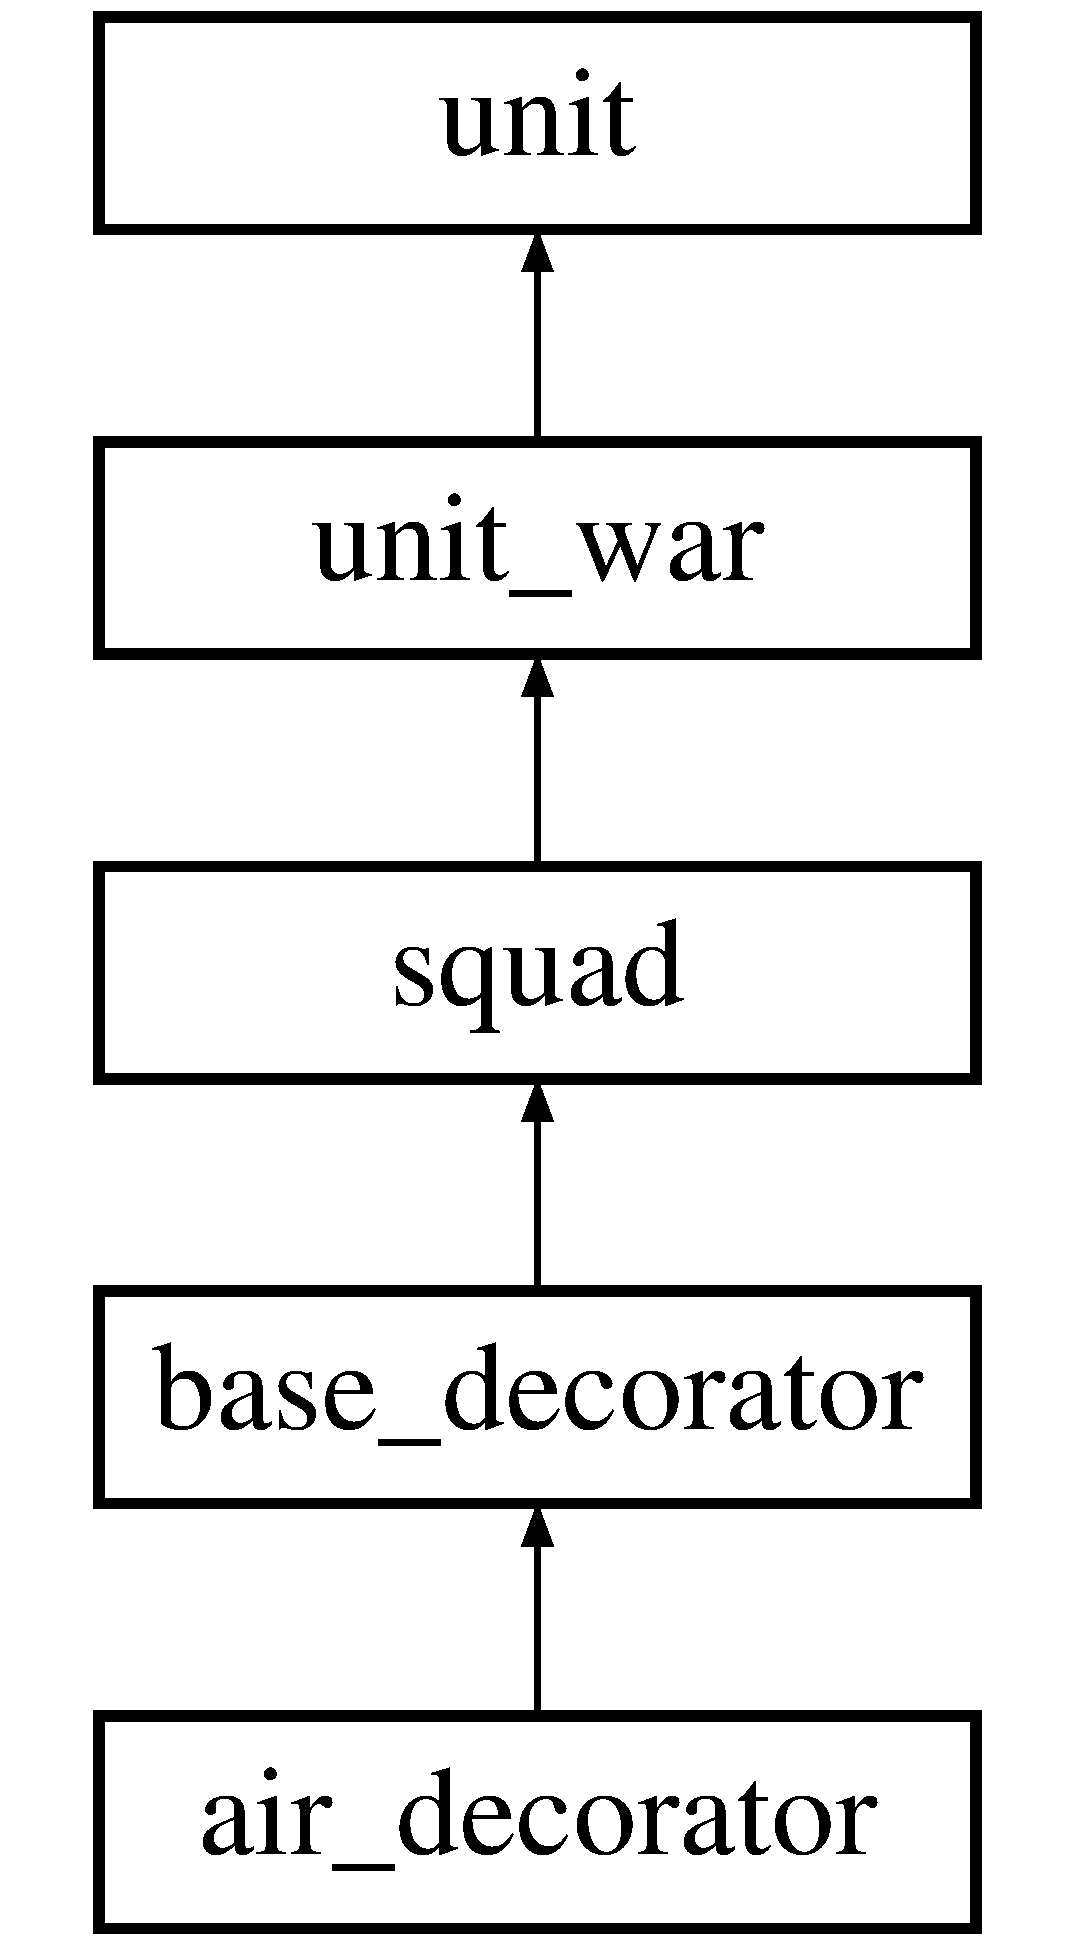
\includegraphics[height=5.000000cm]{classair__decorator}
\end{center}
\end{figure}
\subsection*{Additional Inherited Members}


\subsection{Detailed Description}
brief if army/squad will have to fight in air it will be wrapped in this decorator 

The documentation for this class was generated from the following file\+:\begin{DoxyCompactItemize}
\item 
air\+\_\+decorator.\+h\end{DoxyCompactItemize}

\hypertarget{classair__factory}{}\section{air\+\_\+factory Class Reference}
\label{classair__factory}\index{air\+\_\+factory@{air\+\_\+factory}}


{\ttfamily \#include $<$main\+\_\+lib.\+h$>$}

Inheritance diagram for air\+\_\+factory\+:\begin{figure}[H]
\begin{center}
\leavevmode
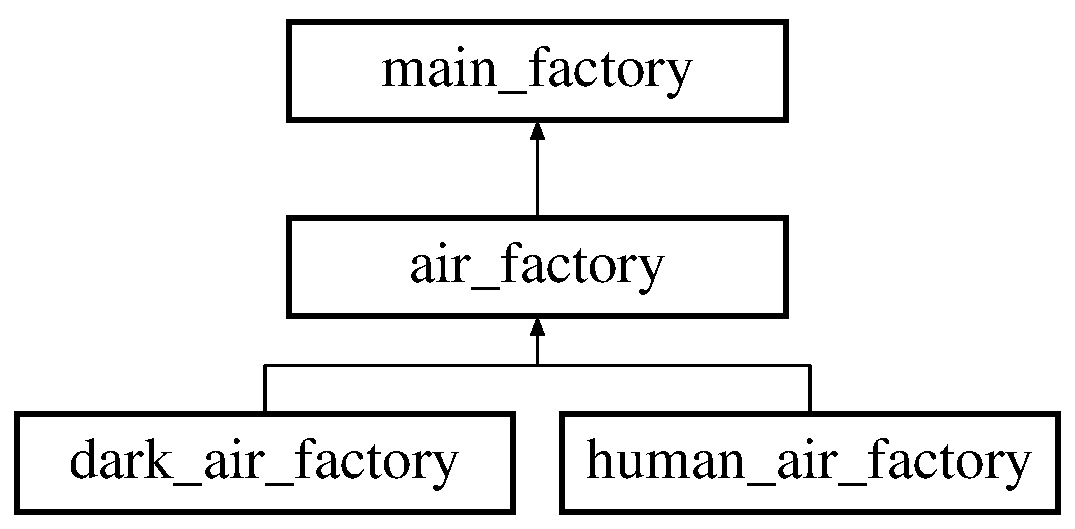
\includegraphics[height=3.000000cm]{classair__factory}
\end{center}
\end{figure}
\subsection*{Public Member Functions}
\begin{DoxyCompactItemize}
\item 
\mbox{\Hypertarget{classair__factory_ac865a7285e585ed10c9f0f46e56276a1}\label{classair__factory_ac865a7285e585ed10c9f0f46e56276a1}} 
virtual \mbox{\hyperlink{classflying__unit}{flying\+\_\+unit}} $\ast$ {\bfseries build\+\_\+bomber} ()
\item 
\mbox{\Hypertarget{classair__factory_a0fec153a637ae326eb914c974e974cf6}\label{classair__factory_a0fec153a637ae326eb914c974e974cf6}} 
virtual \mbox{\hyperlink{classflying__unit}{flying\+\_\+unit}} $\ast$ {\bfseries build\+\_\+fighter} ()
\end{DoxyCompactItemize}
\subsection*{Additional Inherited Members}


\subsection{Detailed Description}
brief special factory for air forces 

The documentation for this class was generated from the following file\+:\begin{DoxyCompactItemize}
\item 
main\+\_\+lib.\+h\end{DoxyCompactItemize}

\hypertarget{classanti__aircraft}{}\section{anti\+\_\+aircraft Class Reference}
\label{classanti__aircraft}\index{anti\+\_\+aircraft@{anti\+\_\+aircraft}}
Inheritance diagram for anti\+\_\+aircraft\+:\begin{figure}[H]
\begin{center}
\leavevmode
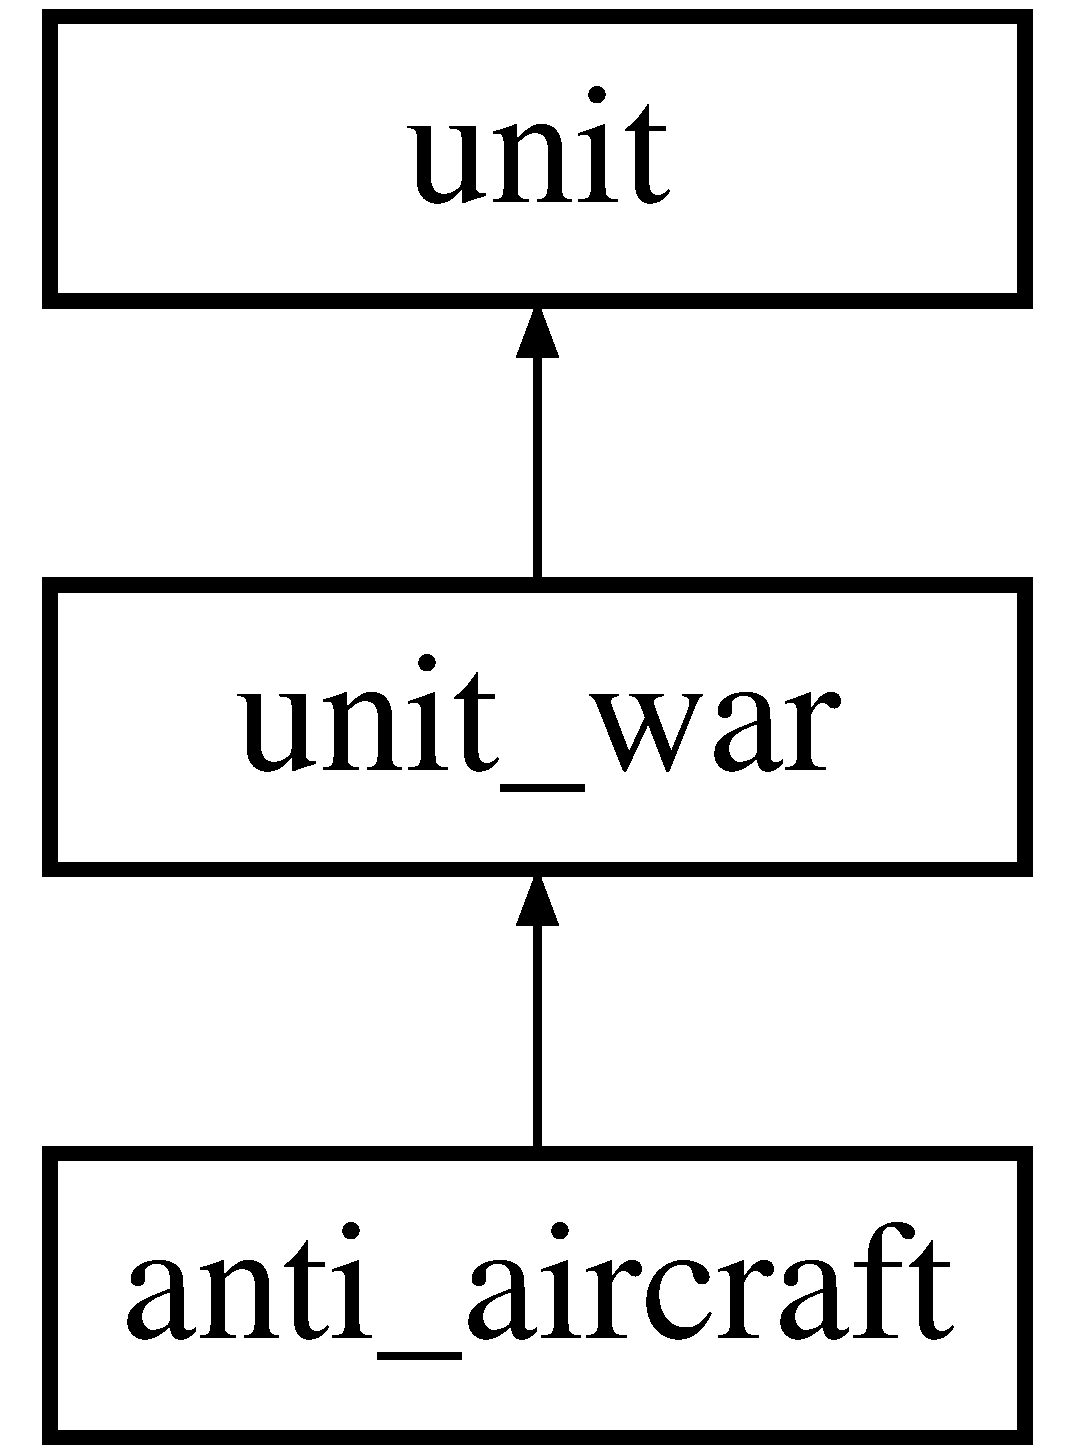
\includegraphics[height=3.000000cm]{classanti__aircraft}
\end{center}
\end{figure}
\subsection*{Public Member Functions}
\begin{DoxyCompactItemize}
\item 
\mbox{\Hypertarget{classanti__aircraft_a6085af8f5b8af4370664a9b6f6196c07}\label{classanti__aircraft_a6085af8f5b8af4370664a9b6f6196c07}} 
void {\bfseries set\+\_\+air\+\_\+deff} (int damage)
\item 
const int \mbox{\hyperlink{classanti__aircraft_aae33f6c35fe31aaefcf0e0cb73838de1}{get\+\_\+air\+\_\+deffence}} () override
\end{DoxyCompactItemize}
\subsection*{Public Attributes}
\begin{DoxyCompactItemize}
\item 
\mbox{\Hypertarget{classanti__aircraft_ae5ea5a9b7db035d6bd628f3bf3a9a0d9}\label{classanti__aircraft_ae5ea5a9b7db035d6bd628f3bf3a9a0d9}} 
int {\bfseries air\+\_\+deff}
\end{DoxyCompactItemize}
\subsection*{Additional Inherited Members}


\subsection{Member Function Documentation}
\mbox{\Hypertarget{classanti__aircraft_aae33f6c35fe31aaefcf0e0cb73838de1}\label{classanti__aircraft_aae33f6c35fe31aaefcf0e0cb73838de1}} 
\index{anti\+\_\+aircraft@{anti\+\_\+aircraft}!get\+\_\+air\+\_\+deffence@{get\+\_\+air\+\_\+deffence}}
\index{get\+\_\+air\+\_\+deffence@{get\+\_\+air\+\_\+deffence}!anti\+\_\+aircraft@{anti\+\_\+aircraft}}
\subsubsection{\texorpdfstring{get\+\_\+air\+\_\+deffence()}{get\_air\_deffence()}}
{\footnotesize\ttfamily const int anti\+\_\+aircraft\+::get\+\_\+air\+\_\+deffence (\begin{DoxyParamCaption}{ }\end{DoxyParamCaption})\hspace{0.3cm}{\ttfamily [inline]}, {\ttfamily [override]}, {\ttfamily [virtual]}}

brief air\+\_\+defence power info \begin{DoxyReturn}{Returns}
air defence power 
\end{DoxyReturn}


Reimplemented from \mbox{\hyperlink{classunit__war_af26f2da420a828230a329339bc9ef805}{unit\+\_\+war}}.



The documentation for this class was generated from the following file\+:\begin{DoxyCompactItemize}
\item 
human\+\_\+tree.\+h\end{DoxyCompactItemize}

\hypertarget{classarmored__mecha}{}\section{armored\+\_\+mecha Class Reference}
\label{classarmored__mecha}\index{armored\+\_\+mecha@{armored\+\_\+mecha}}
Inheritance diagram for armored\+\_\+mecha\+:\begin{figure}[H]
\begin{center}
\leavevmode
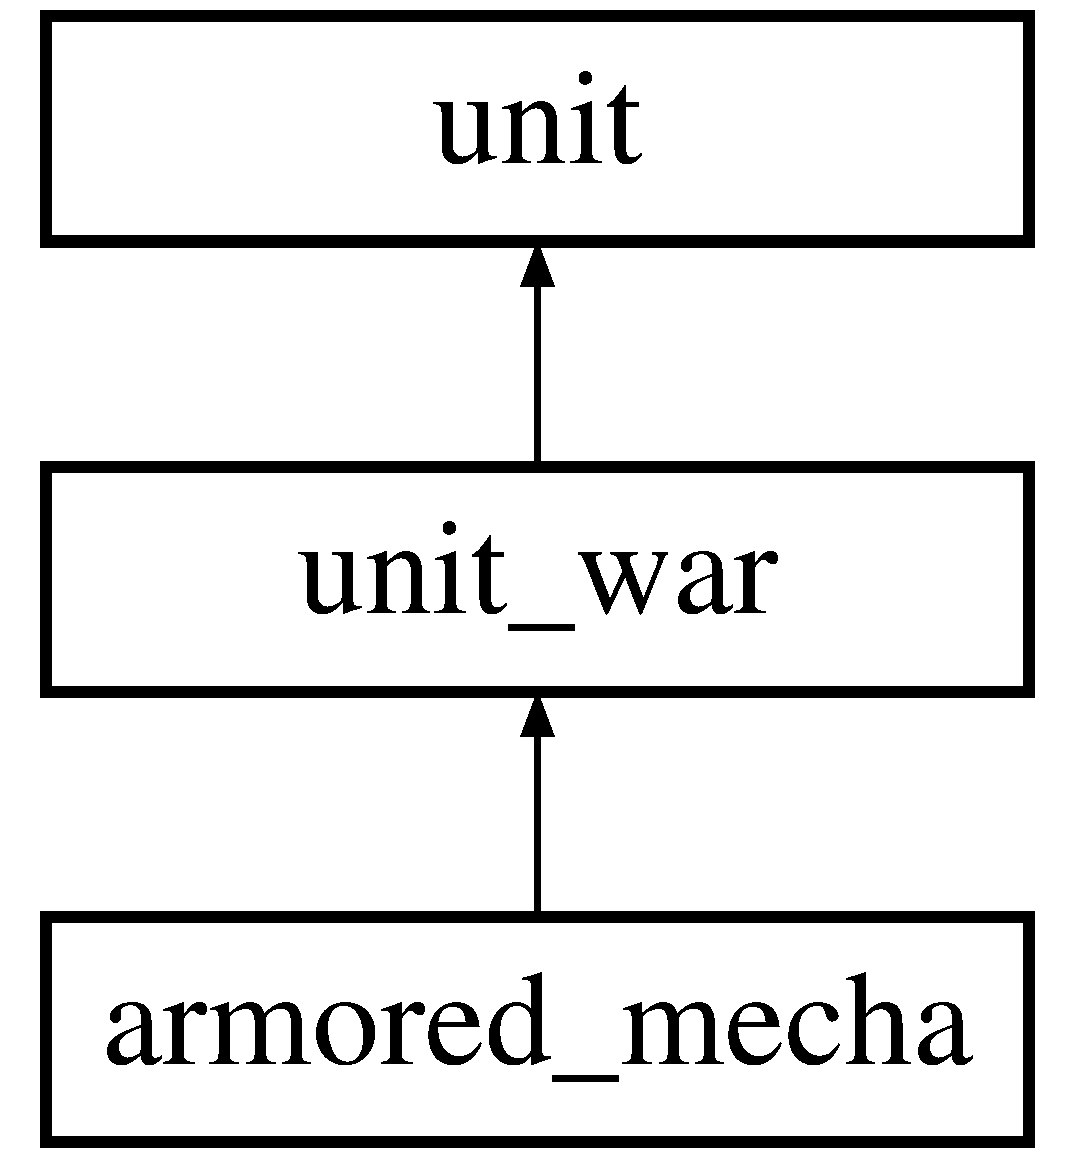
\includegraphics[height=3.000000cm]{classarmored__mecha}
\end{center}
\end{figure}
\subsection*{Additional Inherited Members}


The documentation for this class was generated from the following file\+:\begin{DoxyCompactItemize}
\item 
human\+\_\+tree.\+h\end{DoxyCompactItemize}

\hypertarget{classarmored__solider}{}\section{armored\+\_\+solider Class Reference}
\label{classarmored__solider}\index{armored\+\_\+solider@{armored\+\_\+solider}}
Inheritance diagram for armored\+\_\+solider\+:\begin{figure}[H]
\begin{center}
\leavevmode
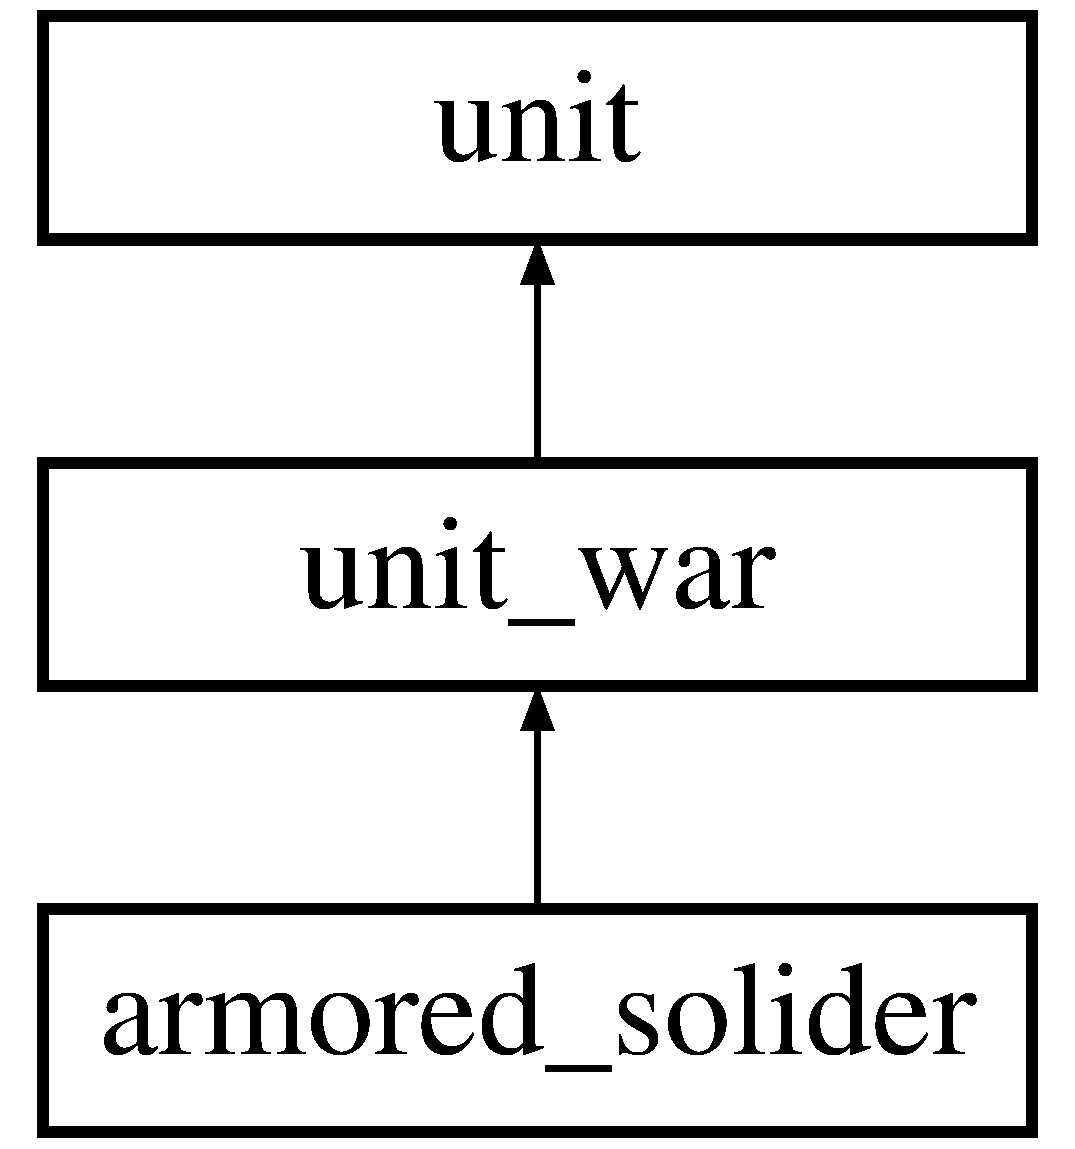
\includegraphics[height=3.000000cm]{classarmored__solider}
\end{center}
\end{figure}
\subsection*{Additional Inherited Members}


The documentation for this class was generated from the following file\+:\begin{DoxyCompactItemize}
\item 
dark\+\_\+fraction.\+h\end{DoxyCompactItemize}

\hypertarget{classarmy}{}\section{army Class Reference}
\label{classarmy}\index{army@{army}}


{\ttfamily \#include $<$army.\+h$>$}

Inheritance diagram for army\+:\begin{figure}[H]
\begin{center}
\leavevmode
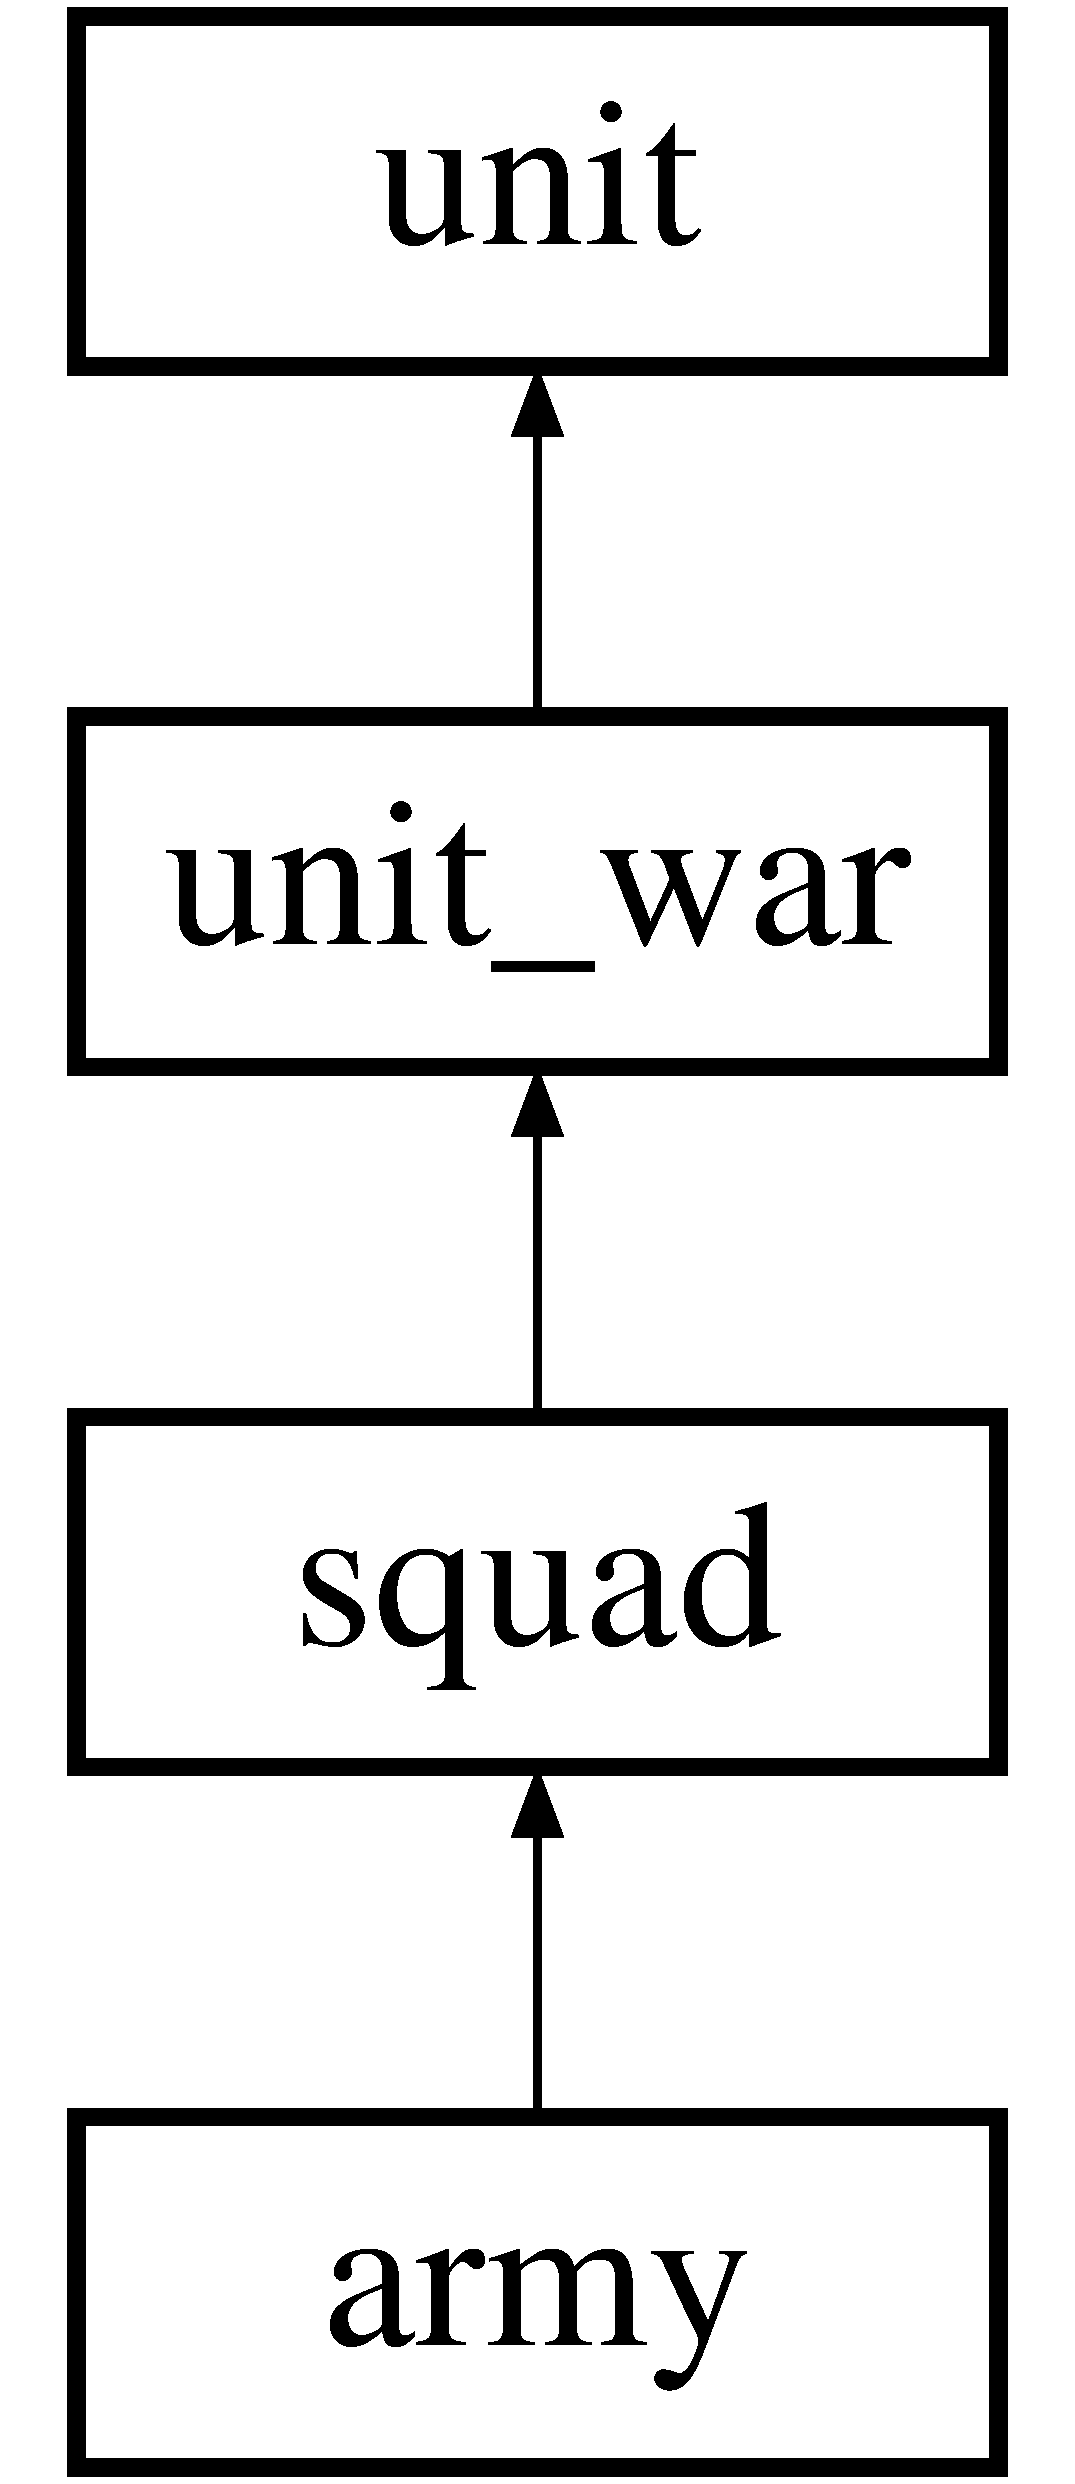
\includegraphics[height=4.000000cm]{classarmy}
\end{center}
\end{figure}
\subsection*{Public Member Functions}
\begin{DoxyCompactItemize}
\item 
\mbox{\Hypertarget{classarmy_a97a8890e39d247b95c14740c8d930e14}\label{classarmy_a97a8890e39d247b95c14740c8d930e14}} 
void {\bfseries enable} ()
\item 
\mbox{\Hypertarget{classarmy_a10e871fc70e584a000bee5abe4f8b6e6}\label{classarmy_a10e871fc70e584a000bee5abe4f8b6e6}} 
void {\bfseries disable} ()
\end{DoxyCompactItemize}
\subsection*{Public Attributes}
\begin{DoxyCompactItemize}
\item 
\mbox{\Hypertarget{classarmy_a58d160ef4574dd273d1e08b62e786a00}\label{classarmy_a58d160ef4574dd273d1e08b62e786a00}} 
bool {\bfseries peace\+\_\+enabled}
\end{DoxyCompactItemize}
\subsection*{Additional Inherited Members}


\subsection{Detailed Description}
brief the last part of composite pattern, can contain units and squads at the same time and also use \char`\"{}peaceful\char`\"{} mode 

The documentation for this class was generated from the following file\+:\begin{DoxyCompactItemize}
\item 
army.\+h\end{DoxyCompactItemize}

\hypertarget{classbase__decorator}{}\section{base\+\_\+decorator Class Reference}
\label{classbase__decorator}\index{base\+\_\+decorator@{base\+\_\+decorator}}


{\ttfamily \#include $<$base\+\_\+decorator.\+h$>$}

Inheritance diagram for base\+\_\+decorator\+:\begin{figure}[H]
\begin{center}
\leavevmode
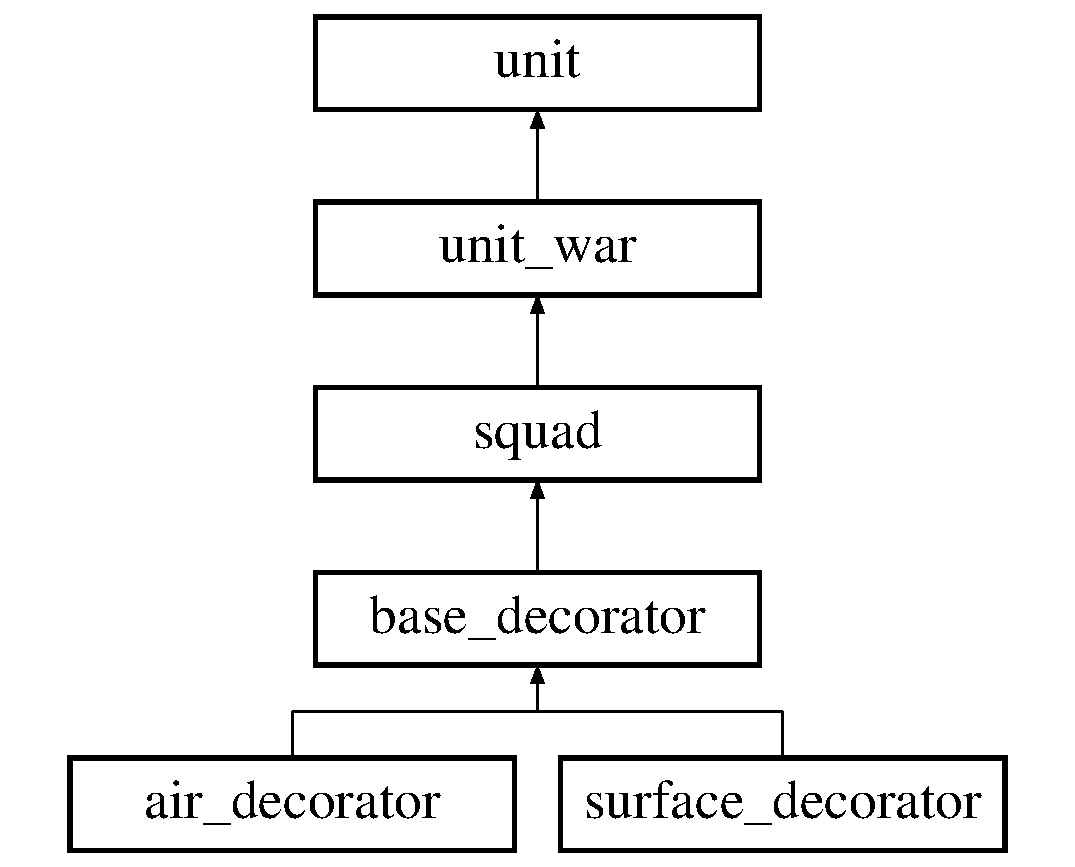
\includegraphics[height=5.000000cm]{classbase__decorator}
\end{center}
\end{figure}
\subsection*{Public Member Functions}
\begin{DoxyCompactItemize}
\item 
\mbox{\Hypertarget{classbase__decorator_a51fc20858a082f22366cd25ad092a630}\label{classbase__decorator_a51fc20858a082f22366cd25ad092a630}} 
{\bfseries base\+\_\+decorator} (\mbox{\hyperlink{classsquad}{squad}} $\ast$s)
\end{DoxyCompactItemize}
\subsection*{Public Attributes}
\begin{DoxyCompactItemize}
\item 
\mbox{\Hypertarget{classbase__decorator_ac7c794ff0e6cb61f2662cc9d691cf237}\label{classbase__decorator_ac7c794ff0e6cb61f2662cc9d691cf237}} 
\mbox{\hyperlink{classsquad}{squad}} $\ast$ {\bfseries wrappee}
\item 
\mbox{\Hypertarget{classbase__decorator_aa91695be3a0986b5937d1ae7ee0b51ad}\label{classbase__decorator_aa91695be3a0986b5937d1ae7ee0b51ad}} 
virtual const int {\bfseries get\+\_\+air\+\_\+power} \{\}
\item 
\mbox{\Hypertarget{classbase__decorator_ad8661d7a99fcb263c85d563e376adf47}\label{classbase__decorator_ad8661d7a99fcb263c85d563e376adf47}} 
virtual const int {\bfseries get\+\_\+surface\+\_\+power} \{\}
\end{DoxyCompactItemize}
\subsection*{Additional Inherited Members}


\subsection{Detailed Description}
brief just base decorator which will be used to wrap a squad or army 

The documentation for this class was generated from the following file\+:\begin{DoxyCompactItemize}
\item 
base\+\_\+decorator.\+h\end{DoxyCompactItemize}

\hypertarget{classbutton}{}\section{button Class Reference}
\label{classbutton}\index{button@{button}}


{\ttfamily \#include $<$simple\+\_\+button.\+h$>$}

\subsection*{Public Attributes}
\begin{DoxyCompactItemize}
\item 
\mbox{\Hypertarget{classbutton_aaf513af175d36f1c6a3ef3e02c91bd01}\label{classbutton_aaf513af175d36f1c6a3ef3e02c91bd01}} 
\mbox{\hyperlink{classcommand}{command}} $\ast$ {\bfseries some\+\_\+command}
\end{DoxyCompactItemize}


\subsection{Detailed Description}
brief S\+Imple version of the buttons, there will be more complicated one with full usage of command pattern later, in release version 

The documentation for this class was generated from the following file\+:\begin{DoxyCompactItemize}
\item 
simple\+\_\+button.\+h\end{DoxyCompactItemize}

\hypertarget{classcommand}{}\section{command Class Reference}
\label{classcommand}\index{command@{command}}


{\ttfamily \#include $<$command.\+h$>$}

Inheritance diagram for command\+:\begin{figure}[H]
\begin{center}
\leavevmode
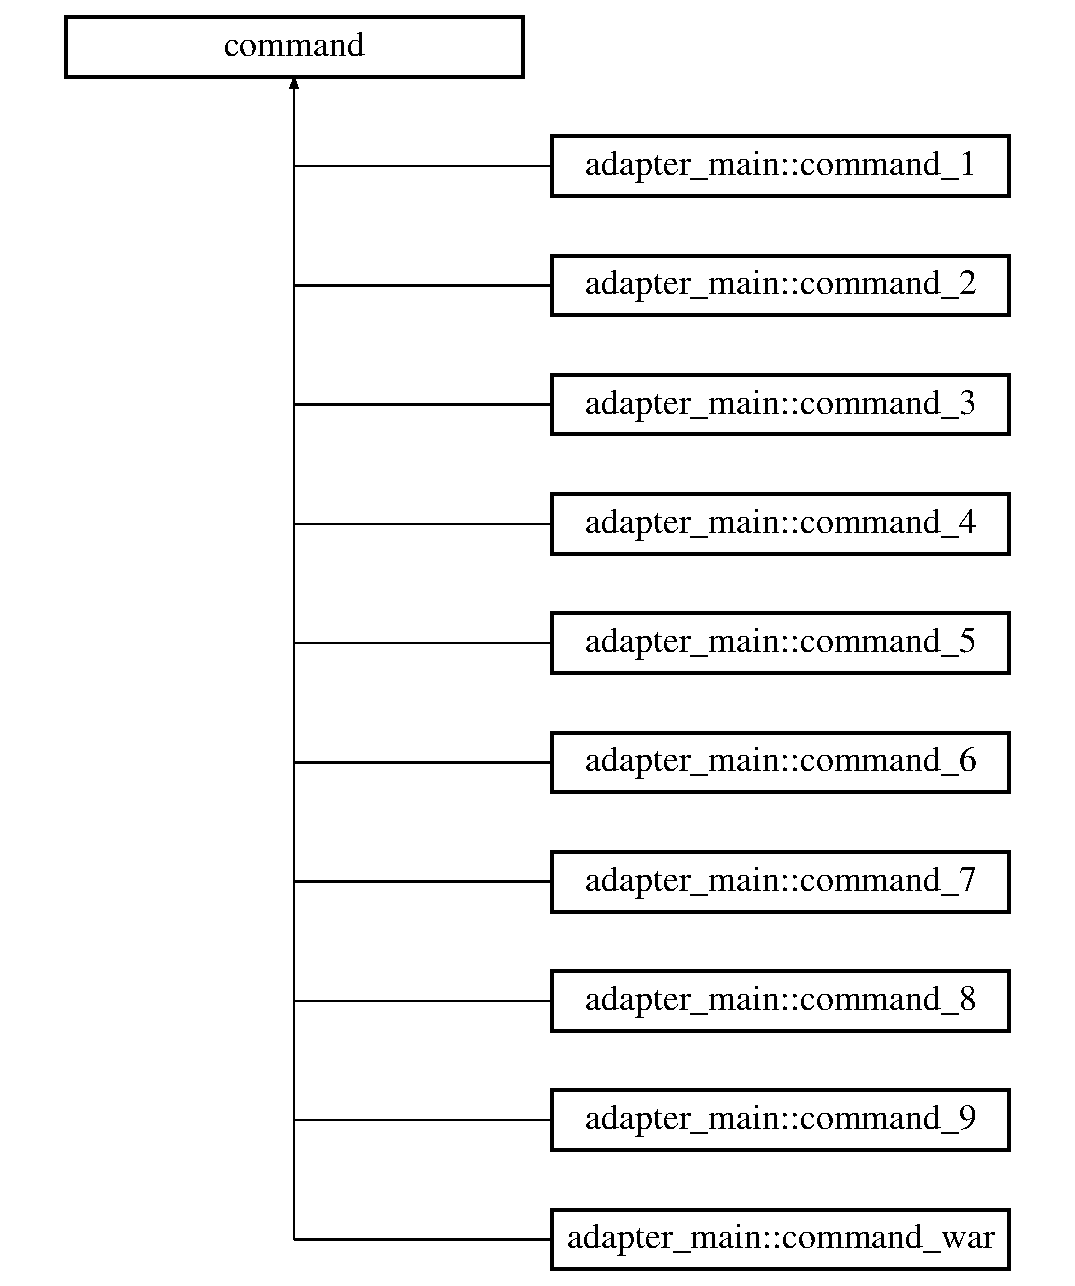
\includegraphics[height=11.000000cm]{classcommand}
\end{center}
\end{figure}
\subsection*{Public Member Functions}
\begin{DoxyCompactItemize}
\item 
\mbox{\Hypertarget{classcommand_af1bc3a3c76e881ead2a750d7a6bbbc57}\label{classcommand_af1bc3a3c76e881ead2a750d7a6bbbc57}} 
{\bfseries command} (\mbox{\hyperlink{classsquad}{squad}} $\ast$\+\_\+num1, \mbox{\hyperlink{classsquad}{squad}} $\ast$\+\_\+num2)
\item 
\mbox{\Hypertarget{classcommand_a0b75272a7b935f50a15d32f88468d400}\label{classcommand_a0b75272a7b935f50a15d32f88468d400}} 
virtual void {\bfseries execute} ()
\item 
\mbox{\Hypertarget{classcommand_ada1e4caeb342f04b40990de4abd9cd08}\label{classcommand_ada1e4caeb342f04b40990de4abd9cd08}} 
virtual void {\bfseries execute} (int i, vector$<$ \mbox{\hyperlink{classmain__unit}{main\+\_\+unit}} $\ast$$>$ \&commander, vector$<$ \mbox{\hyperlink{classsurface__factory}{surface\+\_\+factory}} $\ast$$>$ \&Sfactories, vector$<$ \mbox{\hyperlink{classsurface__factory}{surface\+\_\+factory}} $\ast$$>$ \&sur\+\_\+fact)
\item 
\mbox{\Hypertarget{classcommand_a4ad079d30390f9dd0ba29cc570c82ccf}\label{classcommand_a4ad079d30390f9dd0ba29cc570c82ccf}} 
virtual void {\bfseries execute} (int i, vector$<$ \mbox{\hyperlink{classmain__unit}{main\+\_\+unit}} $\ast$$>$ \&commander, vector$<$ \mbox{\hyperlink{classair__factory}{air\+\_\+factory}} $\ast$$>$ \&Afactories, vector$<$ \mbox{\hyperlink{classair__factory}{air\+\_\+factory}} $\ast$$>$ \&air\+\_\+fact)
\item 
\mbox{\Hypertarget{classcommand_aa7bc94fa393e4b052581d34153b2d246}\label{classcommand_aa7bc94fa393e4b052581d34153b2d246}} 
virtual void {\bfseries execute} (vector$<$ \mbox{\hyperlink{classsurface__factory}{surface\+\_\+factory}} $\ast$$>$ \&Sfactories, vector$<$ \mbox{\hyperlink{classair__factory}{air\+\_\+factory}} $\ast$$>$ \&Afactories, vector$<$ \mbox{\hyperlink{classunit}{unit}} $\ast$$>$ \&all\+\_\+units)
\item 
\mbox{\Hypertarget{classcommand_aa4cc58bbcfbaae8e272af56f2a151ef1}\label{classcommand_aa4cc58bbcfbaae8e272af56f2a151ef1}} 
virtual void {\bfseries execute} (vector$<$ \mbox{\hyperlink{classair__factory}{air\+\_\+factory}} $\ast$$>$ \&Afactories, vector$<$ \mbox{\hyperlink{classunit}{unit}} $\ast$$>$ \&all\+\_\+units)
\item 
\mbox{\Hypertarget{classcommand_a1de78d90b3c4ee0532dc67e348c760ea}\label{classcommand_a1de78d90b3c4ee0532dc67e348c760ea}} 
virtual void {\bfseries execute} (vector$<$ \mbox{\hyperlink{classsurface__factory}{surface\+\_\+factory}} $\ast$$>$ \&Sfactories, vector$<$ \mbox{\hyperlink{classunit}{unit}} $\ast$$>$ \&all\+\_\+units)
\end{DoxyCompactItemize}
\subsection*{Protected Attributes}
\begin{DoxyCompactItemize}
\item 
\mbox{\Hypertarget{classcommand_a30a3ade7522d7b33716ac27fb50412a1}\label{classcommand_a30a3ade7522d7b33716ac27fb50412a1}} 
\mbox{\hyperlink{classsquad}{squad}} $\ast$ {\bfseries num1}
\item 
\mbox{\Hypertarget{classcommand_a4cac3d92834e0f4fc1cad5ffb54755d6}\label{classcommand_a4cac3d92834e0f4fc1cad5ffb54755d6}} 
\mbox{\hyperlink{classsquad}{squad}} $\ast$ {\bfseries num2}
\end{DoxyCompactItemize}


\subsection{Detailed Description}
brief A command pattern main class 

The documentation for this class was generated from the following file\+:\begin{DoxyCompactItemize}
\item 
command.\+h\end{DoxyCompactItemize}

\hypertarget{classadapter__main_1_1command__1}{}\section{adapter\+\_\+main\+:\+:command\+\_\+1 Class Reference}
\label{classadapter__main_1_1command__1}\index{adapter\+\_\+main\+::command\+\_\+1@{adapter\+\_\+main\+::command\+\_\+1}}
Inheritance diagram for adapter\+\_\+main\+:\+:command\+\_\+1\+:\begin{figure}[H]
\begin{center}
\leavevmode
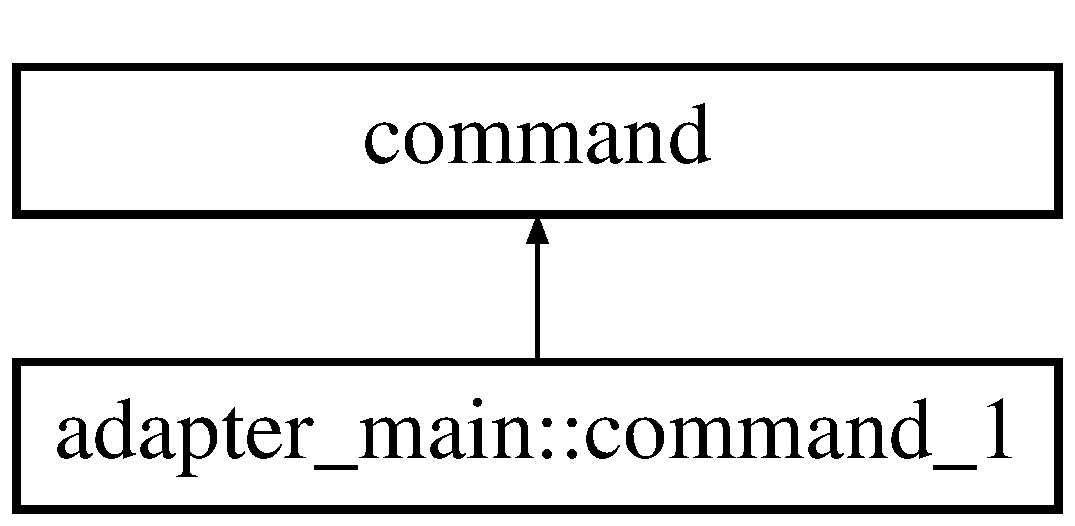
\includegraphics[height=2.000000cm]{classadapter__main_1_1command__1}
\end{center}
\end{figure}
\subsection*{Public Member Functions}
\begin{DoxyCompactItemize}
\item 
\mbox{\Hypertarget{classadapter__main_1_1command__1_a30a0d3a507b6986c4821bc7808abe759}\label{classadapter__main_1_1command__1_a30a0d3a507b6986c4821bc7808abe759}} 
void {\bfseries execute} (int i, vector$<$ \mbox{\hyperlink{classmain__unit}{main\+\_\+unit}} $\ast$$>$ \&commander, vector$<$ \mbox{\hyperlink{classsurface__factory}{surface\+\_\+factory}} $\ast$$>$ \&Sfactories, vector$<$ \mbox{\hyperlink{classsurface__factory}{surface\+\_\+factory}} $\ast$$>$ \&sur\+\_\+fact) override
\end{DoxyCompactItemize}
\subsection*{Additional Inherited Members}


The documentation for this class was generated from the following file\+:\begin{DoxyCompactItemize}
\item 
client\+\_\+adapter.\+h\end{DoxyCompactItemize}

\hypertarget{classadapter__main_1_1command__2}{}\section{adapter\+\_\+main\+:\+:command\+\_\+2 Class Reference}
\label{classadapter__main_1_1command__2}\index{adapter\+\_\+main\+::command\+\_\+2@{adapter\+\_\+main\+::command\+\_\+2}}
Inheritance diagram for adapter\+\_\+main\+:\+:command\+\_\+2\+:\begin{figure}[H]
\begin{center}
\leavevmode
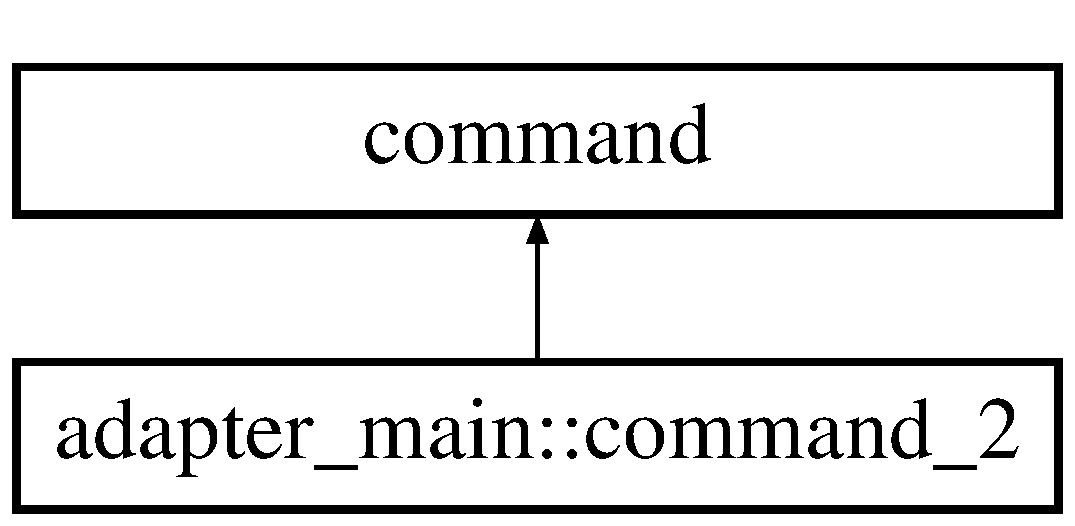
\includegraphics[height=2.000000cm]{classadapter__main_1_1command__2}
\end{center}
\end{figure}
\subsection*{Public Member Functions}
\begin{DoxyCompactItemize}
\item 
\mbox{\Hypertarget{classadapter__main_1_1command__2_a2a2d647942a41f0aabc903bfb78b40fd}\label{classadapter__main_1_1command__2_a2a2d647942a41f0aabc903bfb78b40fd}} 
void {\bfseries execute} (int i, vector$<$ \mbox{\hyperlink{classmain__unit}{main\+\_\+unit}} $\ast$$>$ \&commander, vector$<$ \mbox{\hyperlink{classair__factory}{air\+\_\+factory}} $\ast$$>$ \&Afactories, vector$<$ \mbox{\hyperlink{classair__factory}{air\+\_\+factory}} $\ast$$>$ \&air\+\_\+fact) override
\end{DoxyCompactItemize}
\subsection*{Additional Inherited Members}


The documentation for this class was generated from the following file\+:\begin{DoxyCompactItemize}
\item 
client\+\_\+adapter.\+h\end{DoxyCompactItemize}

\hypertarget{classadapter__main_1_1command__3}{}\section{adapter\+\_\+main\+:\+:command\+\_\+3 Class Reference}
\label{classadapter__main_1_1command__3}\index{adapter\+\_\+main\+::command\+\_\+3@{adapter\+\_\+main\+::command\+\_\+3}}
Inheritance diagram for adapter\+\_\+main\+:\+:command\+\_\+3\+:\begin{figure}[H]
\begin{center}
\leavevmode
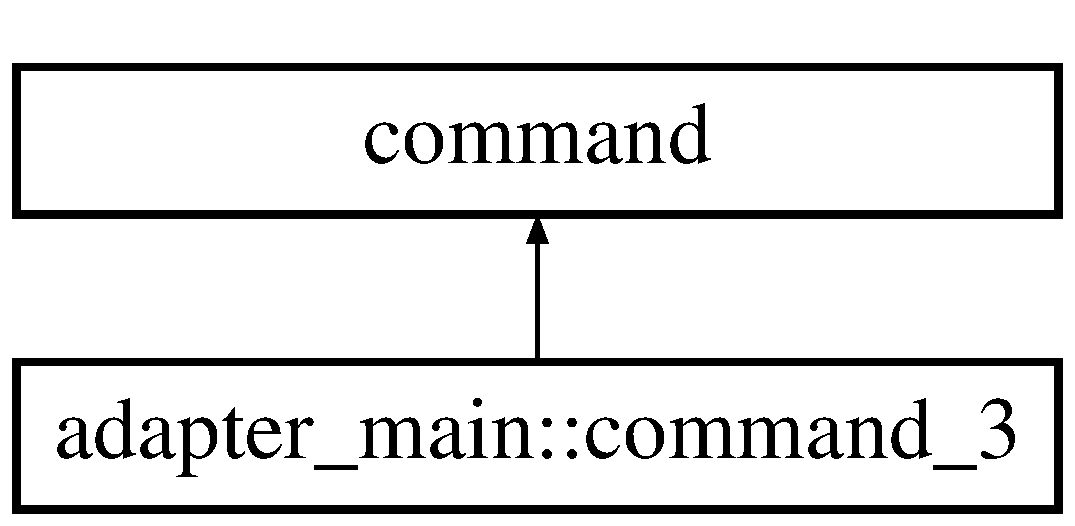
\includegraphics[height=2.000000cm]{classadapter__main_1_1command__3}
\end{center}
\end{figure}
\subsection*{Public Member Functions}
\begin{DoxyCompactItemize}
\item 
\mbox{\Hypertarget{classadapter__main_1_1command__3_a54f0628f4eaacf4a4423899b96a9ba32}\label{classadapter__main_1_1command__3_a54f0628f4eaacf4a4423899b96a9ba32}} 
void {\bfseries execute} (vector$<$ \mbox{\hyperlink{classsurface__factory}{surface\+\_\+factory}} $\ast$$>$ \&Sfactories, vector$<$ \mbox{\hyperlink{classair__factory}{air\+\_\+factory}} $\ast$$>$ \&Afactories, vector$<$ \mbox{\hyperlink{classunit}{unit}} $\ast$$>$ \&all\+\_\+units) override
\end{DoxyCompactItemize}
\subsection*{Additional Inherited Members}


The documentation for this class was generated from the following file\+:\begin{DoxyCompactItemize}
\item 
client\+\_\+adapter.\+h\end{DoxyCompactItemize}

\hypertarget{classadapter__main_1_1command__4}{}\section{adapter\+\_\+main\+:\+:command\+\_\+4 Class Reference}
\label{classadapter__main_1_1command__4}\index{adapter\+\_\+main\+::command\+\_\+4@{adapter\+\_\+main\+::command\+\_\+4}}
Inheritance diagram for adapter\+\_\+main\+:\+:command\+\_\+4\+:\begin{figure}[H]
\begin{center}
\leavevmode
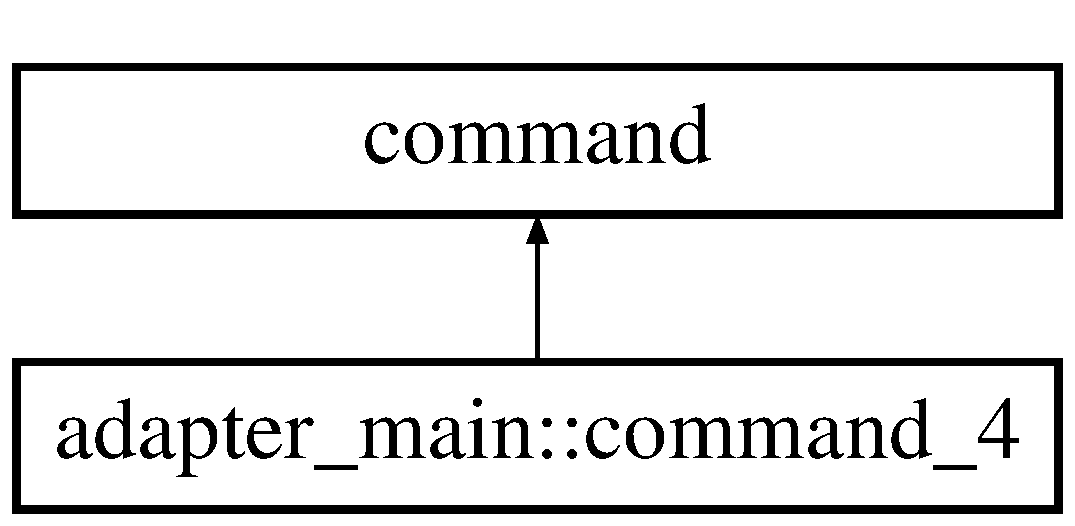
\includegraphics[height=2.000000cm]{classadapter__main_1_1command__4}
\end{center}
\end{figure}
\subsection*{Public Member Functions}
\begin{DoxyCompactItemize}
\item 
\mbox{\Hypertarget{classadapter__main_1_1command__4_ad42743cae2ca979bc520bf0e3840018d}\label{classadapter__main_1_1command__4_ad42743cae2ca979bc520bf0e3840018d}} 
void {\bfseries execute} (vector$<$ \mbox{\hyperlink{classair__factory}{air\+\_\+factory}} $\ast$$>$ \&Afactories, vector$<$ \mbox{\hyperlink{classunit}{unit}} $\ast$$>$ \&all\+\_\+units) override
\end{DoxyCompactItemize}
\subsection*{Additional Inherited Members}


The documentation for this class was generated from the following file\+:\begin{DoxyCompactItemize}
\item 
client\+\_\+adapter.\+h\end{DoxyCompactItemize}

\hypertarget{classadapter__main_1_1command__5}{}\section{adapter\+\_\+main\+:\+:command\+\_\+5 Class Reference}
\label{classadapter__main_1_1command__5}\index{adapter\+\_\+main\+::command\+\_\+5@{adapter\+\_\+main\+::command\+\_\+5}}
Inheritance diagram for adapter\+\_\+main\+:\+:command\+\_\+5\+:\begin{figure}[H]
\begin{center}
\leavevmode
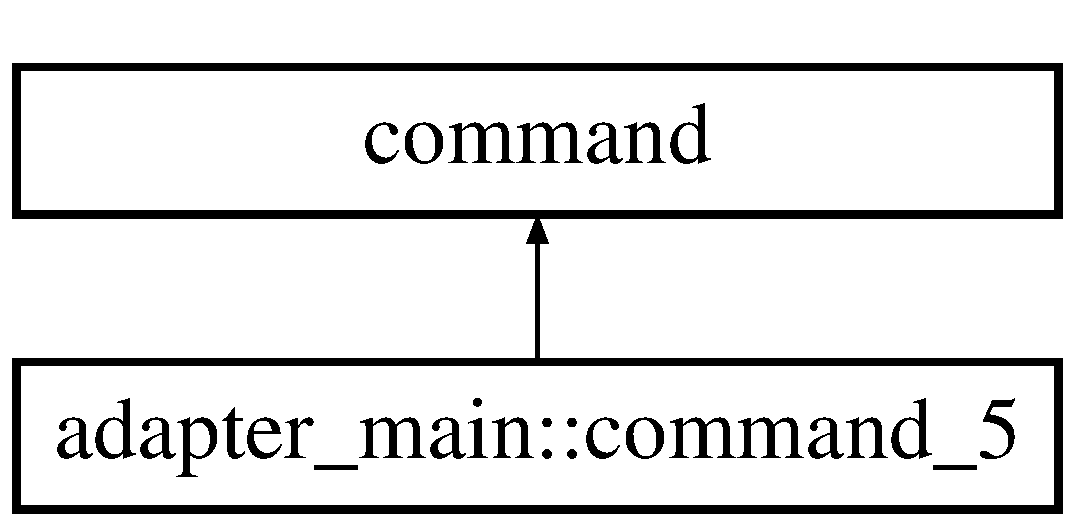
\includegraphics[height=2.000000cm]{classadapter__main_1_1command__5}
\end{center}
\end{figure}
\subsection*{Public Member Functions}
\begin{DoxyCompactItemize}
\item 
\mbox{\Hypertarget{classadapter__main_1_1command__5_a6ec76ad103fdb25233b613bb009c0b46}\label{classadapter__main_1_1command__5_a6ec76ad103fdb25233b613bb009c0b46}} 
void {\bfseries execute} (vector$<$ \mbox{\hyperlink{classair__factory}{air\+\_\+factory}} $\ast$$>$ \&Afactories, vector$<$ \mbox{\hyperlink{classunit}{unit}} $\ast$$>$ \&all\+\_\+units) override
\end{DoxyCompactItemize}
\subsection*{Additional Inherited Members}


The documentation for this class was generated from the following file\+:\begin{DoxyCompactItemize}
\item 
client\+\_\+adapter.\+h\end{DoxyCompactItemize}

\hypertarget{classadapter__main_1_1command__6}{}\section{adapter\+\_\+main\+:\+:command\+\_\+6 Class Reference}
\label{classadapter__main_1_1command__6}\index{adapter\+\_\+main\+::command\+\_\+6@{adapter\+\_\+main\+::command\+\_\+6}}
Inheritance diagram for adapter\+\_\+main\+:\+:command\+\_\+6\+:\begin{figure}[H]
\begin{center}
\leavevmode
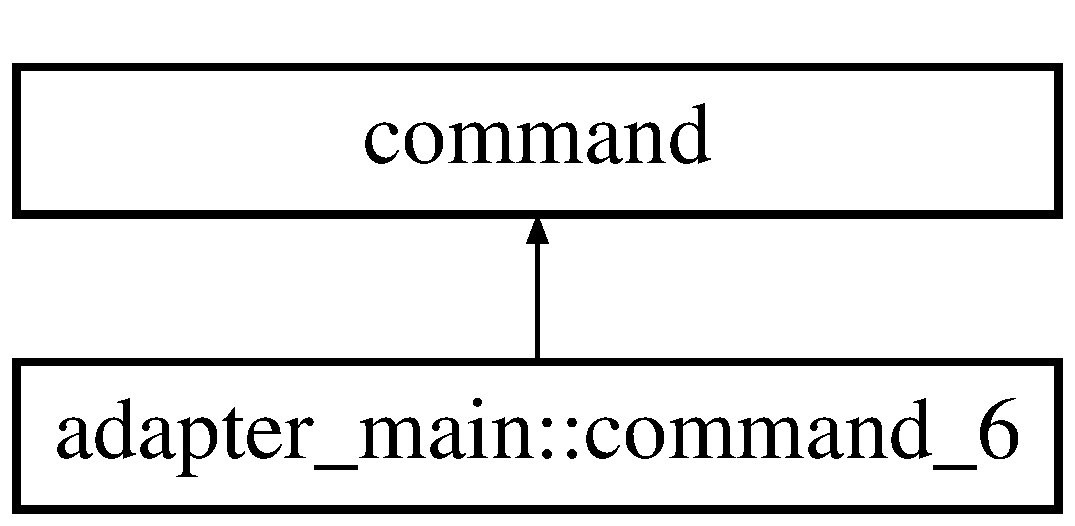
\includegraphics[height=2.000000cm]{classadapter__main_1_1command__6}
\end{center}
\end{figure}
\subsection*{Public Member Functions}
\begin{DoxyCompactItemize}
\item 
\mbox{\Hypertarget{classadapter__main_1_1command__6_a2c084b732f91f56576d4bbaef9835380}\label{classadapter__main_1_1command__6_a2c084b732f91f56576d4bbaef9835380}} 
void {\bfseries execute} (vector$<$ \mbox{\hyperlink{classsurface__factory}{surface\+\_\+factory}} $\ast$$>$ \&Sfactories, vector$<$ \mbox{\hyperlink{classunit}{unit}} $\ast$$>$ \&all\+\_\+units) override
\end{DoxyCompactItemize}
\subsection*{Additional Inherited Members}


The documentation for this class was generated from the following file\+:\begin{DoxyCompactItemize}
\item 
client\+\_\+adapter.\+h\end{DoxyCompactItemize}

\hypertarget{classadapter__main_1_1command__7}{}\section{adapter\+\_\+main\+:\+:command\+\_\+7 Class Reference}
\label{classadapter__main_1_1command__7}\index{adapter\+\_\+main\+::command\+\_\+7@{adapter\+\_\+main\+::command\+\_\+7}}
Inheritance diagram for adapter\+\_\+main\+:\+:command\+\_\+7\+:\begin{figure}[H]
\begin{center}
\leavevmode
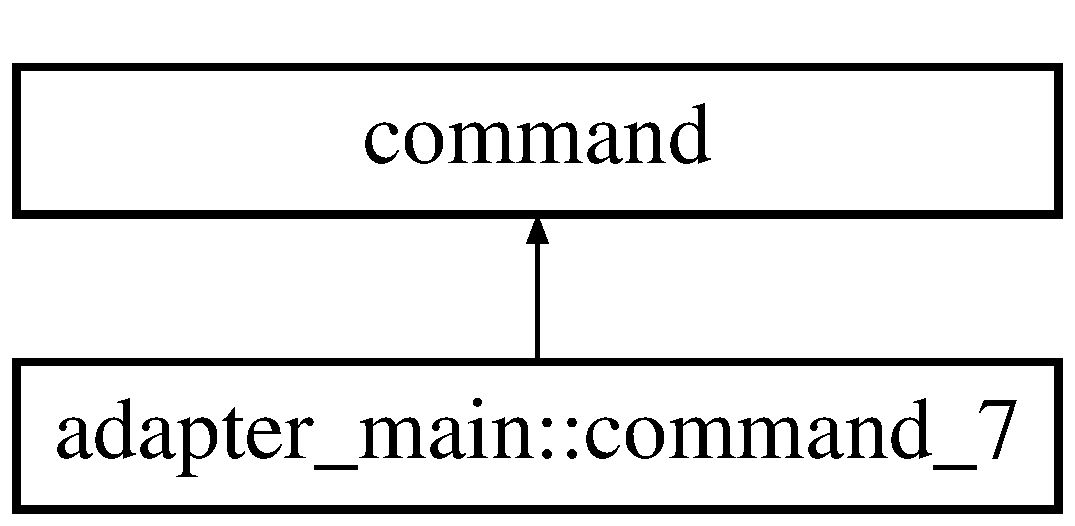
\includegraphics[height=2.000000cm]{classadapter__main_1_1command__7}
\end{center}
\end{figure}
\subsection*{Public Member Functions}
\begin{DoxyCompactItemize}
\item 
\mbox{\Hypertarget{classadapter__main_1_1command__7_a71fac9c70e9725e59f106195f8888e36}\label{classadapter__main_1_1command__7_a71fac9c70e9725e59f106195f8888e36}} 
void {\bfseries execute} (vector$<$ \mbox{\hyperlink{classsurface__factory}{surface\+\_\+factory}} $\ast$$>$ \&Sfactories, vector$<$ \mbox{\hyperlink{classunit}{unit}} $\ast$$>$ \&all\+\_\+units) override
\end{DoxyCompactItemize}
\subsection*{Additional Inherited Members}


The documentation for this class was generated from the following file\+:\begin{DoxyCompactItemize}
\item 
client\+\_\+adapter.\+h\end{DoxyCompactItemize}

\hypertarget{classadapter__main_1_1command__8}{}\section{adapter\+\_\+main\+:\+:command\+\_\+8 Class Reference}
\label{classadapter__main_1_1command__8}\index{adapter\+\_\+main\+::command\+\_\+8@{adapter\+\_\+main\+::command\+\_\+8}}
Inheritance diagram for adapter\+\_\+main\+:\+:command\+\_\+8\+:\begin{figure}[H]
\begin{center}
\leavevmode
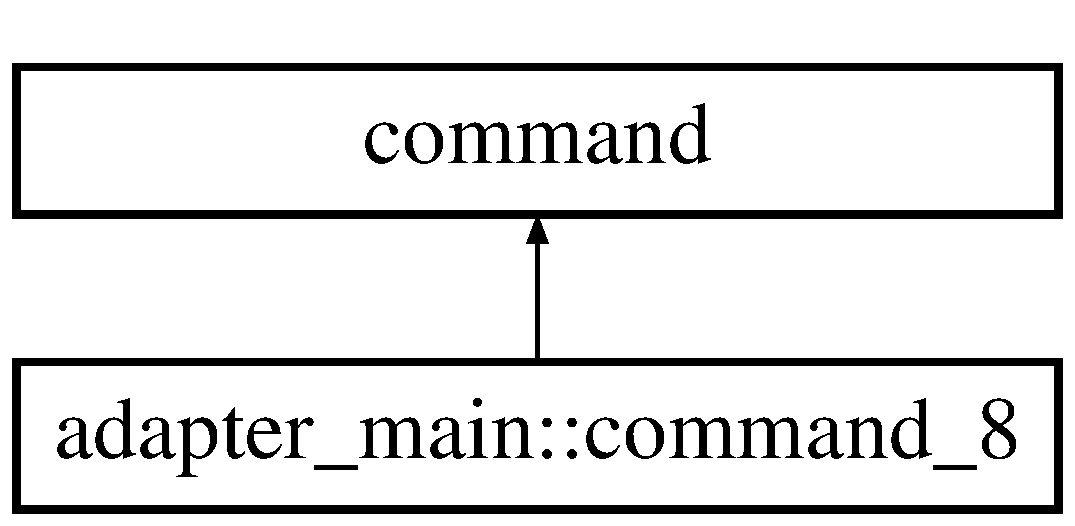
\includegraphics[height=2.000000cm]{classadapter__main_1_1command__8}
\end{center}
\end{figure}
\subsection*{Public Member Functions}
\begin{DoxyCompactItemize}
\item 
\mbox{\Hypertarget{classadapter__main_1_1command__8_aaa7095401388176c1e53d3cd21f6b264}\label{classadapter__main_1_1command__8_aaa7095401388176c1e53d3cd21f6b264}} 
void {\bfseries execute} (vector$<$ \mbox{\hyperlink{classsurface__factory}{surface\+\_\+factory}} $\ast$$>$ \&Sfactories, vector$<$ \mbox{\hyperlink{classunit}{unit}} $\ast$$>$ \&all\+\_\+units) override
\end{DoxyCompactItemize}
\subsection*{Additional Inherited Members}


The documentation for this class was generated from the following file\+:\begin{DoxyCompactItemize}
\item 
client\+\_\+adapter.\+h\end{DoxyCompactItemize}

\hypertarget{classadapter__main_1_1command__9}{}\section{adapter\+\_\+main\+:\+:command\+\_\+9 Class Reference}
\label{classadapter__main_1_1command__9}\index{adapter\+\_\+main\+::command\+\_\+9@{adapter\+\_\+main\+::command\+\_\+9}}
Inheritance diagram for adapter\+\_\+main\+:\+:command\+\_\+9\+:\begin{figure}[H]
\begin{center}
\leavevmode
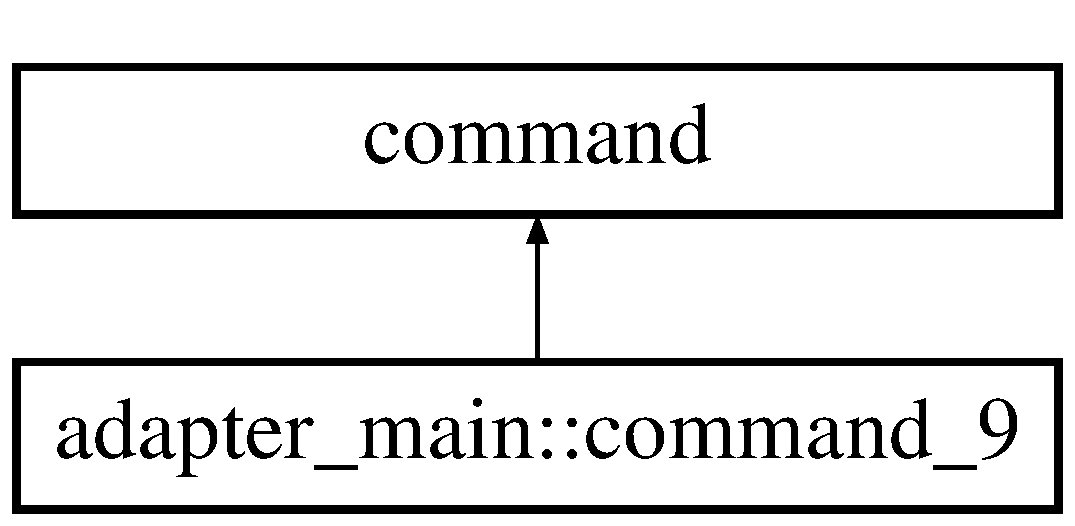
\includegraphics[height=2.000000cm]{classadapter__main_1_1command__9}
\end{center}
\end{figure}
\subsection*{Public Member Functions}
\begin{DoxyCompactItemize}
\item 
\mbox{\Hypertarget{classadapter__main_1_1command__9_a74655d2394d36bfe34e0fa11d969fcbd}\label{classadapter__main_1_1command__9_a74655d2394d36bfe34e0fa11d969fcbd}} 
void {\bfseries execute} (vector$<$ \mbox{\hyperlink{classsurface__factory}{surface\+\_\+factory}} $\ast$$>$ \&Sfactories, vector$<$ \mbox{\hyperlink{classunit}{unit}} $\ast$$>$ \&all\+\_\+units) override
\end{DoxyCompactItemize}
\subsection*{Additional Inherited Members}


The documentation for this class was generated from the following file\+:\begin{DoxyCompactItemize}
\item 
client\+\_\+adapter.\+h\end{DoxyCompactItemize}

\hypertarget{classadapter__main_1_1command__war}{}\section{adapter\+\_\+main\+:\+:command\+\_\+war Class Reference}
\label{classadapter__main_1_1command__war}\index{adapter\+\_\+main\+::command\+\_\+war@{adapter\+\_\+main\+::command\+\_\+war}}
Inheritance diagram for adapter\+\_\+main\+:\+:command\+\_\+war\+:\begin{figure}[H]
\begin{center}
\leavevmode
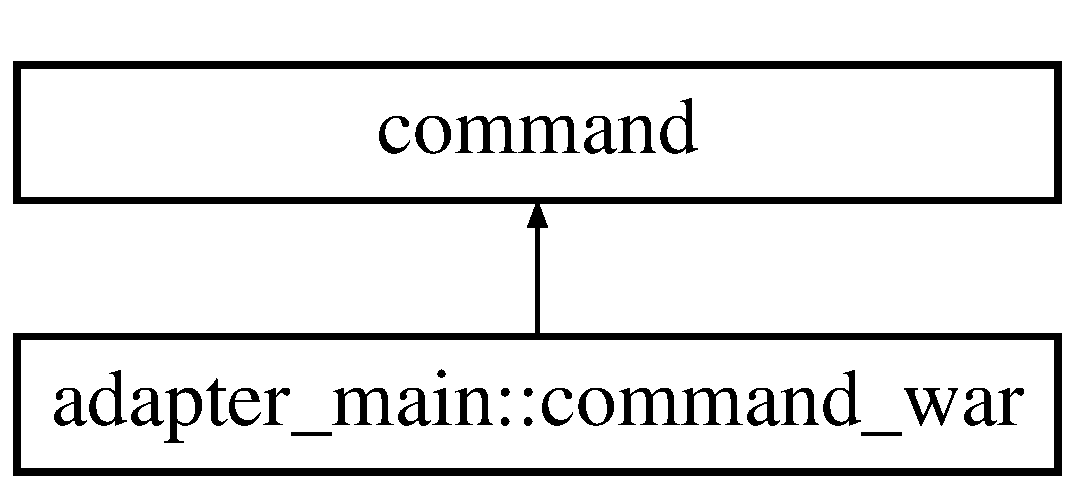
\includegraphics[height=2.000000cm]{classadapter__main_1_1command__war}
\end{center}
\end{figure}
\subsection*{Public Member Functions}
\begin{DoxyCompactItemize}
\item 
\mbox{\Hypertarget{classadapter__main_1_1command__war_aeaf39a056c309d07f7ab1284faf7a994}\label{classadapter__main_1_1command__war_aeaf39a056c309d07f7ab1284faf7a994}} 
{\bfseries command\+\_\+war} (\mbox{\hyperlink{classsquad}{squad}} $\ast$one, \mbox{\hyperlink{classsquad}{squad}} $\ast$two)
\item 
\mbox{\Hypertarget{classadapter__main_1_1command__war_a521f1f6a3ba4c96214d5167f0df25913}\label{classadapter__main_1_1command__war_a521f1f6a3ba4c96214d5167f0df25913}} 
void {\bfseries execute} () override
\end{DoxyCompactItemize}
\subsection*{Additional Inherited Members}


The documentation for this class was generated from the following file\+:\begin{DoxyCompactItemize}
\item 
client\+\_\+adapter.\+h\end{DoxyCompactItemize}

\hypertarget{classdark__air__factory}{}\section{dark\+\_\+air\+\_\+factory Class Reference}
\label{classdark__air__factory}\index{dark\+\_\+air\+\_\+factory@{dark\+\_\+air\+\_\+factory}}
Inheritance diagram for dark\+\_\+air\+\_\+factory\+:\begin{figure}[H]
\begin{center}
\leavevmode
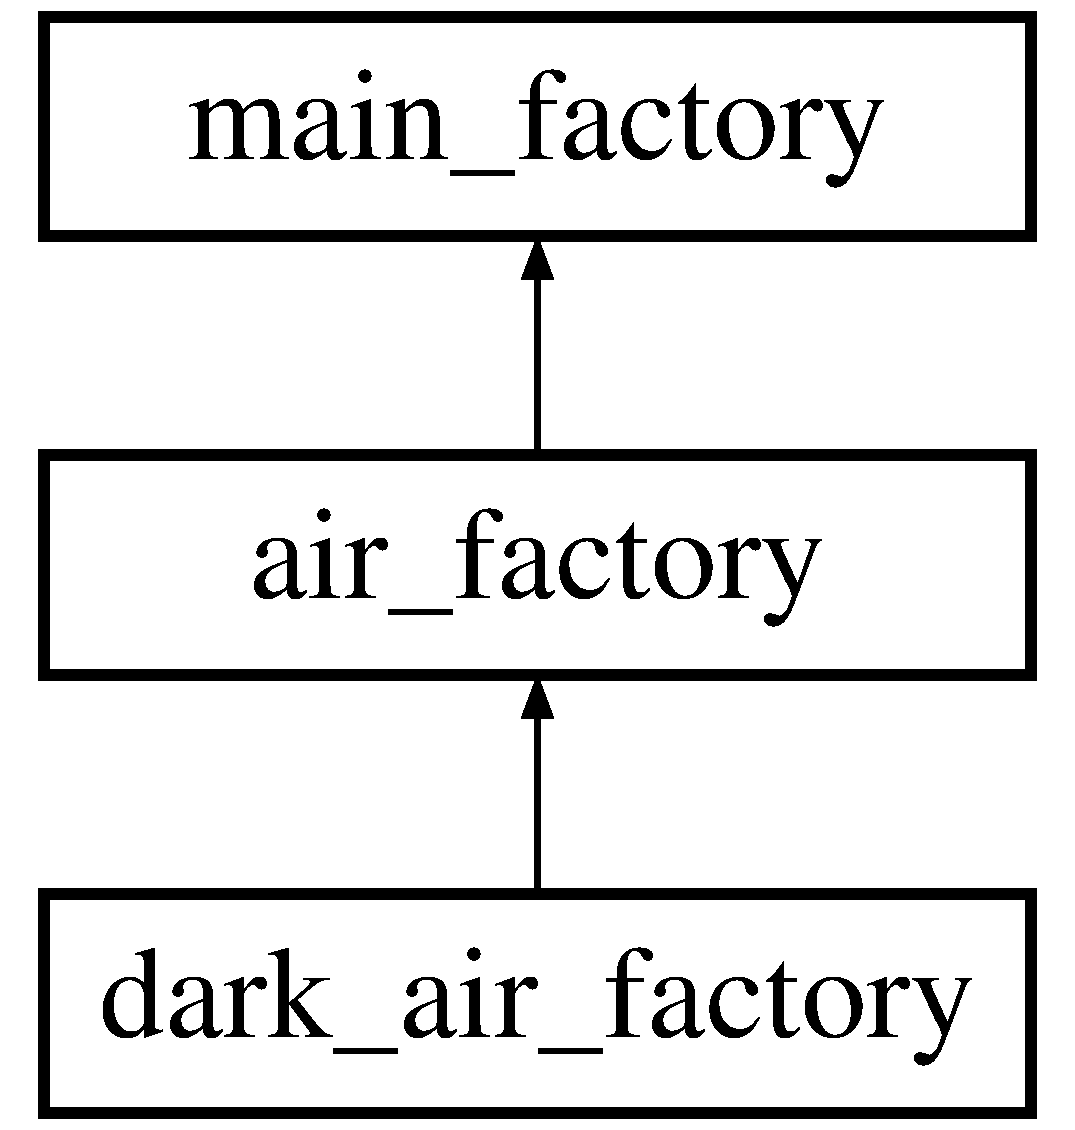
\includegraphics[height=3.000000cm]{classdark__air__factory}
\end{center}
\end{figure}
\subsection*{Public Member Functions}
\begin{DoxyCompactItemize}
\item 
\mbox{\Hypertarget{classdark__air__factory_a2d621db522bf5712d3adfecc5f8dfc80}\label{classdark__air__factory_a2d621db522bf5712d3adfecc5f8dfc80}} 
\mbox{\hyperlink{classdark__bomber}{dark\+\_\+bomber}} $\ast$ {\bfseries build\+\_\+bomber} () override
\item 
\mbox{\Hypertarget{classdark__air__factory_a66b398b461de02ff27e140e689503dfd}\label{classdark__air__factory_a66b398b461de02ff27e140e689503dfd}} 
\mbox{\hyperlink{classdark__air__fighter}{dark\+\_\+air\+\_\+fighter}} $\ast$ {\bfseries build\+\_\+fighter} () override
\item 
\mbox{\hyperlink{classdark__engineer}{dark\+\_\+engineer}} $\ast$ \mbox{\hyperlink{classdark__air__factory_aaabd99e42553b5514b2fae2967bc3248}{build\+\_\+engineer}} () override
\end{DoxyCompactItemize}
\subsection*{Additional Inherited Members}


\subsection{Member Function Documentation}
\mbox{\Hypertarget{classdark__air__factory_aaabd99e42553b5514b2fae2967bc3248}\label{classdark__air__factory_aaabd99e42553b5514b2fae2967bc3248}} 
\index{dark\+\_\+air\+\_\+factory@{dark\+\_\+air\+\_\+factory}!build\+\_\+engineer@{build\+\_\+engineer}}
\index{build\+\_\+engineer@{build\+\_\+engineer}!dark\+\_\+air\+\_\+factory@{dark\+\_\+air\+\_\+factory}}
\subsubsection{\texorpdfstring{build\+\_\+engineer()}{build\_engineer()}}
{\footnotesize\ttfamily \mbox{\hyperlink{classdark__engineer}{dark\+\_\+engineer}}$\ast$ dark\+\_\+air\+\_\+factory\+::build\+\_\+engineer (\begin{DoxyParamCaption}{ }\end{DoxyParamCaption})\hspace{0.3cm}{\ttfamily [inline]}, {\ttfamily [override]}, {\ttfamily [virtual]}}

func to build an engineer \begin{DoxyReturn}{Returns}
new engineer 
\end{DoxyReturn}


Reimplemented from \mbox{\hyperlink{classmain__factory_ac970fe346638331722123f2bb240b590}{main\+\_\+factory}}.



The documentation for this class was generated from the following file\+:\begin{DoxyCompactItemize}
\item 
dark\+\_\+fraction.\+h\end{DoxyCompactItemize}

\hypertarget{classdark__air__fighter}{}\section{dark\+\_\+air\+\_\+fighter Class Reference}
\label{classdark__air__fighter}\index{dark\+\_\+air\+\_\+fighter@{dark\+\_\+air\+\_\+fighter}}
Inheritance diagram for dark\+\_\+air\+\_\+fighter\+:\begin{figure}[H]
\begin{center}
\leavevmode
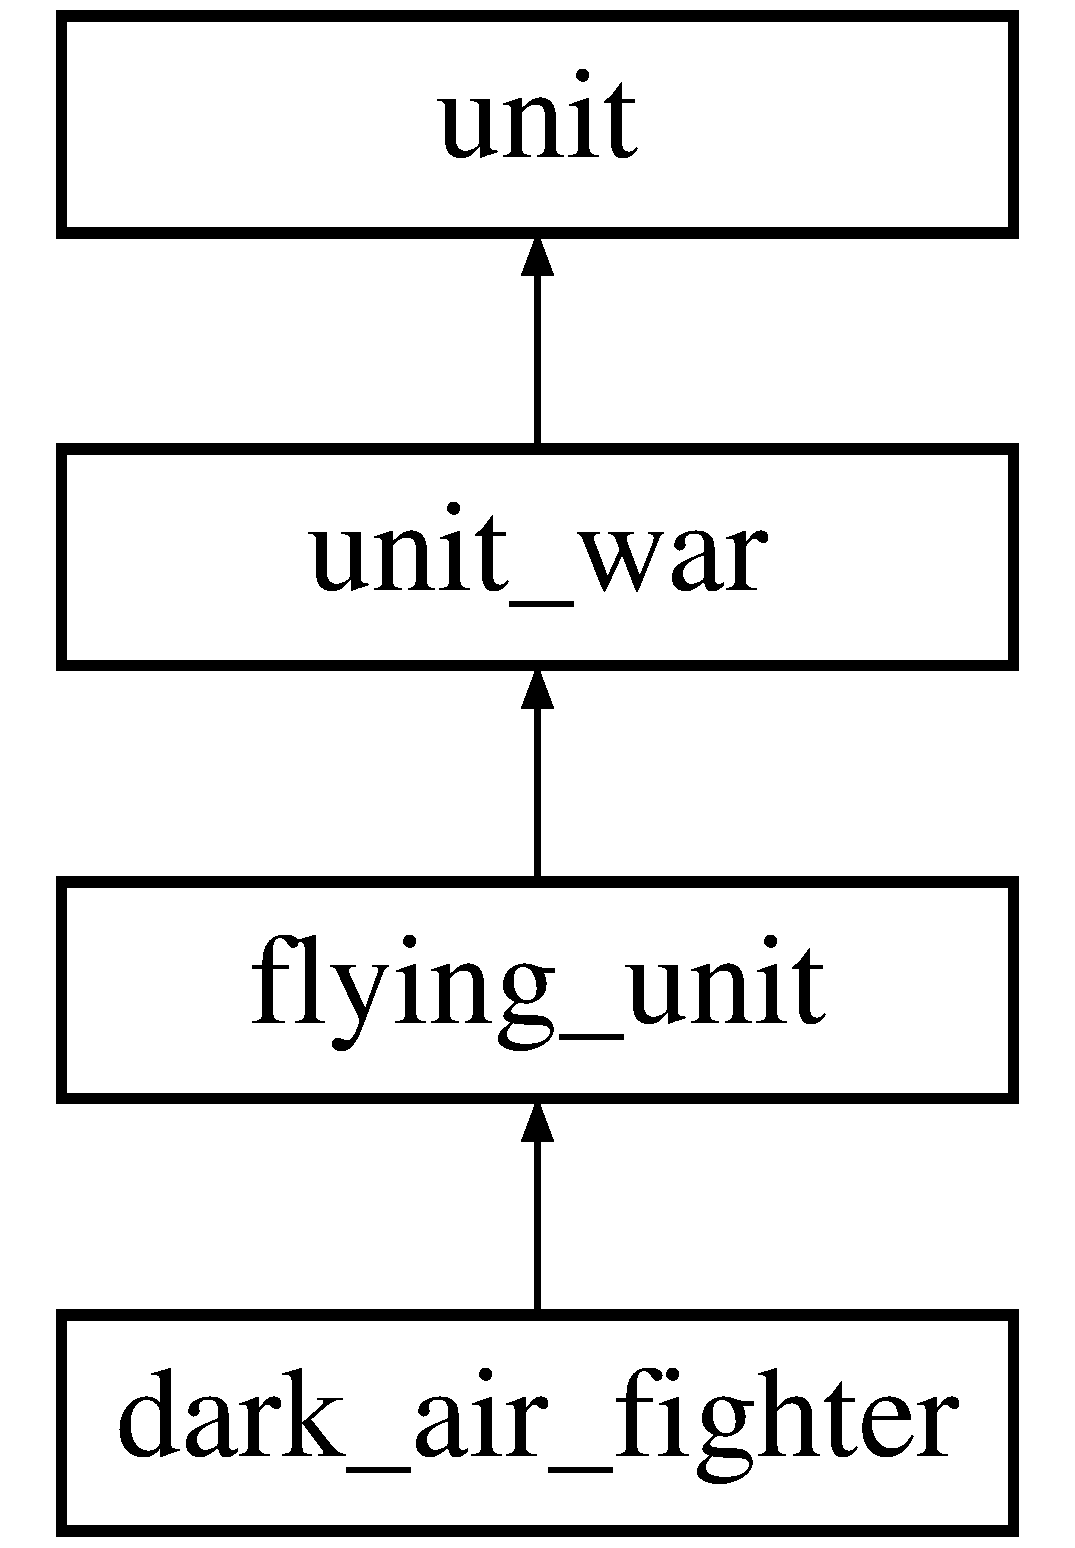
\includegraphics[height=4.000000cm]{classdark__air__fighter}
\end{center}
\end{figure}
\subsection*{Additional Inherited Members}


The documentation for this class was generated from the following file\+:\begin{DoxyCompactItemize}
\item 
dark\+\_\+fraction.\+h\end{DoxyCompactItemize}

\hypertarget{classdark__anti__aircraft}{}\section{dark\+\_\+anti\+\_\+aircraft Class Reference}
\label{classdark__anti__aircraft}\index{dark\+\_\+anti\+\_\+aircraft@{dark\+\_\+anti\+\_\+aircraft}}
Inheritance diagram for dark\+\_\+anti\+\_\+aircraft\+:\begin{figure}[H]
\begin{center}
\leavevmode
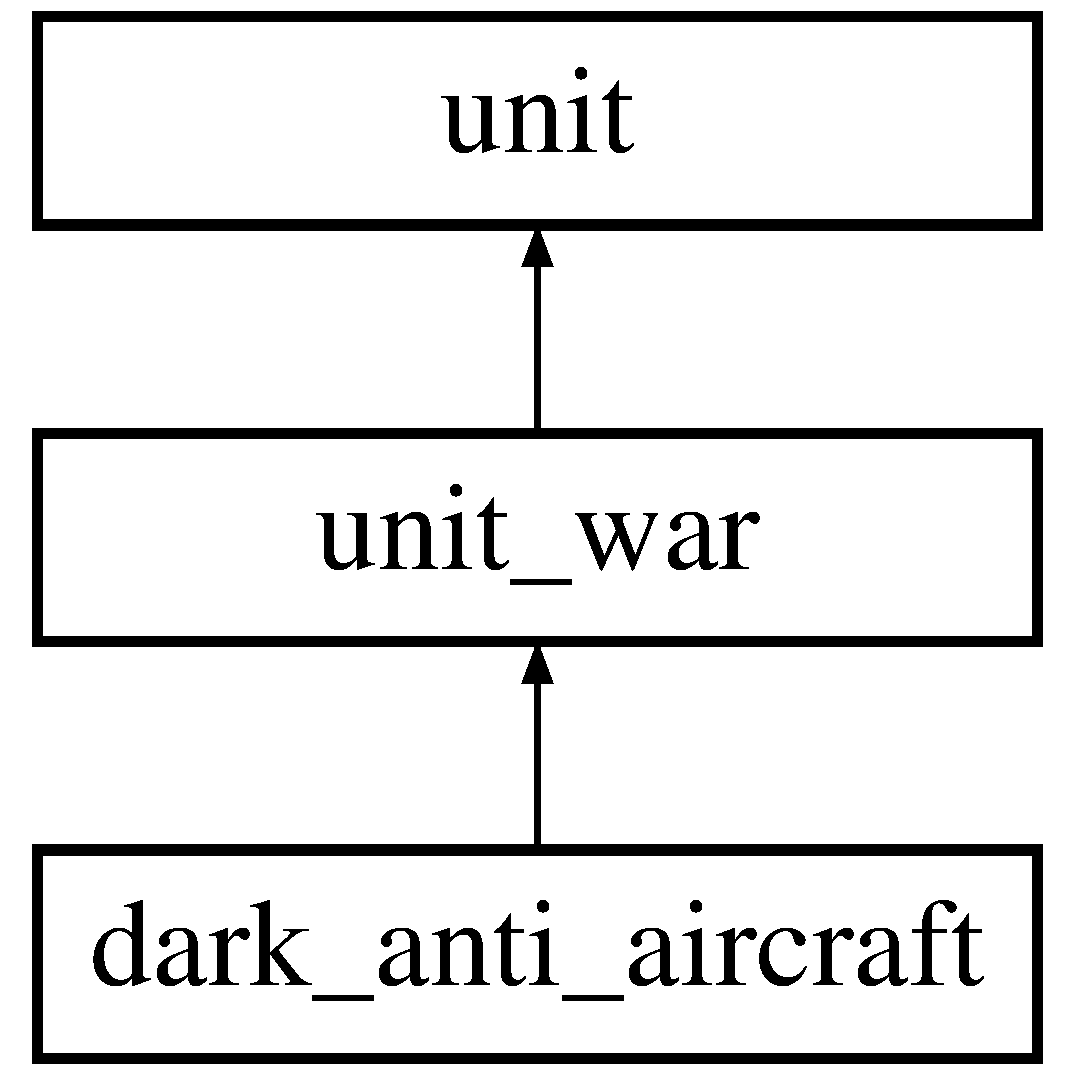
\includegraphics[height=3.000000cm]{classdark__anti__aircraft}
\end{center}
\end{figure}
\subsection*{Public Member Functions}
\begin{DoxyCompactItemize}
\item 
\mbox{\Hypertarget{classdark__anti__aircraft_a0bb8cd743c83023a2fbcd0e2c4d42cda}\label{classdark__anti__aircraft_a0bb8cd743c83023a2fbcd0e2c4d42cda}} 
void {\bfseries set\+\_\+air\+\_\+deff} (int damage)
\item 
const int \mbox{\hyperlink{classdark__anti__aircraft_a572ddd2093ff6e8479392b788a5be231}{get\+\_\+air\+\_\+deffence}} () override
\end{DoxyCompactItemize}
\subsection*{Public Attributes}
\begin{DoxyCompactItemize}
\item 
\mbox{\Hypertarget{classdark__anti__aircraft_a1030e667c38840cbc2f5473c5d5a0a23}\label{classdark__anti__aircraft_a1030e667c38840cbc2f5473c5d5a0a23}} 
int {\bfseries air\+\_\+deff}
\end{DoxyCompactItemize}
\subsection*{Additional Inherited Members}


\subsection{Member Function Documentation}
\mbox{\Hypertarget{classdark__anti__aircraft_a572ddd2093ff6e8479392b788a5be231}\label{classdark__anti__aircraft_a572ddd2093ff6e8479392b788a5be231}} 
\index{dark\+\_\+anti\+\_\+aircraft@{dark\+\_\+anti\+\_\+aircraft}!get\+\_\+air\+\_\+deffence@{get\+\_\+air\+\_\+deffence}}
\index{get\+\_\+air\+\_\+deffence@{get\+\_\+air\+\_\+deffence}!dark\+\_\+anti\+\_\+aircraft@{dark\+\_\+anti\+\_\+aircraft}}
\subsubsection{\texorpdfstring{get\+\_\+air\+\_\+deffence()}{get\_air\_deffence()}}
{\footnotesize\ttfamily const int dark\+\_\+anti\+\_\+aircraft\+::get\+\_\+air\+\_\+deffence (\begin{DoxyParamCaption}{ }\end{DoxyParamCaption})\hspace{0.3cm}{\ttfamily [inline]}, {\ttfamily [override]}, {\ttfamily [virtual]}}

brief air\+\_\+defence power info \begin{DoxyReturn}{Returns}
air defence power 
\end{DoxyReturn}


Reimplemented from \mbox{\hyperlink{classunit__war_af26f2da420a828230a329339bc9ef805}{unit\+\_\+war}}.



The documentation for this class was generated from the following file\+:\begin{DoxyCompactItemize}
\item 
dark\+\_\+fraction.\+h\end{DoxyCompactItemize}

\hypertarget{classdark__bomber}{}\section{dark\+\_\+bomber Class Reference}
\label{classdark__bomber}\index{dark\+\_\+bomber@{dark\+\_\+bomber}}
Inheritance diagram for dark\+\_\+bomber\+:\begin{figure}[H]
\begin{center}
\leavevmode
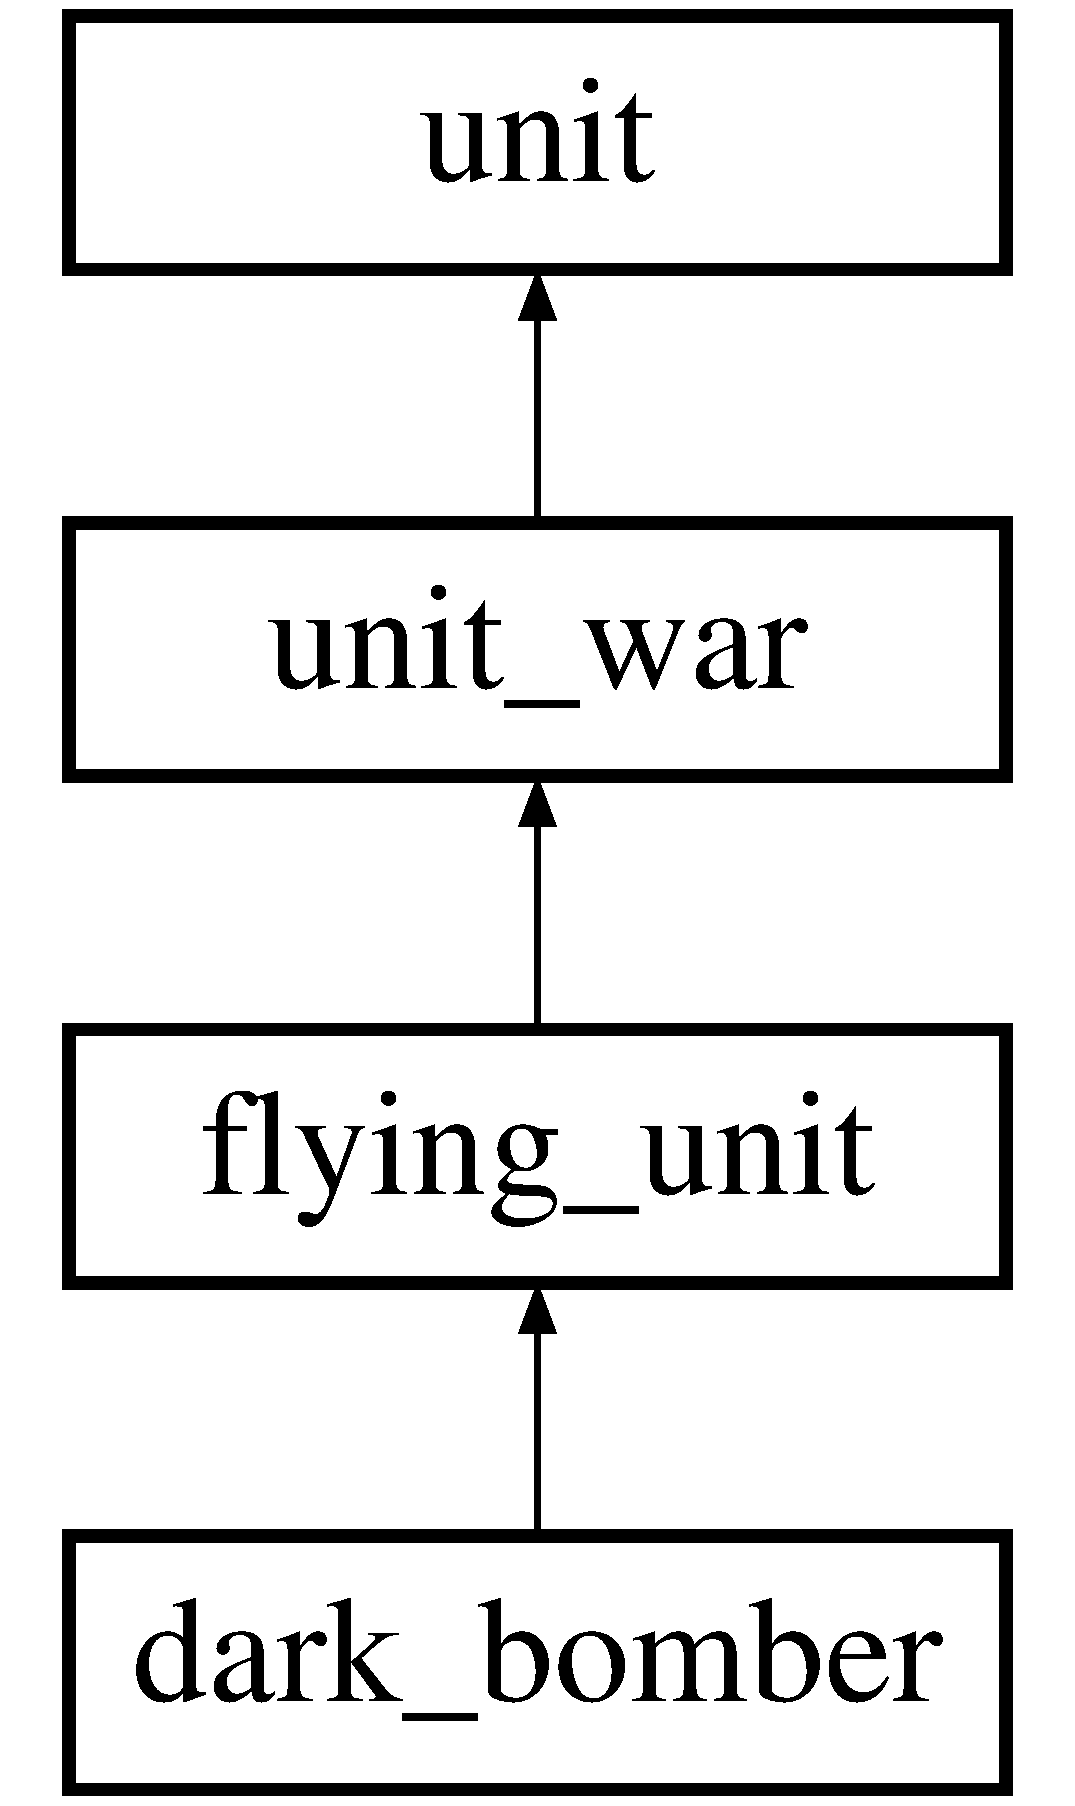
\includegraphics[height=4.000000cm]{classdark__bomber}
\end{center}
\end{figure}
\subsection*{Additional Inherited Members}


The documentation for this class was generated from the following file\+:\begin{DoxyCompactItemize}
\item 
dark\+\_\+fraction.\+h\end{DoxyCompactItemize}

\hypertarget{classdark__engineer}{}\section{dark\+\_\+engineer Class Reference}
\label{classdark__engineer}\index{dark\+\_\+engineer@{dark\+\_\+engineer}}
Inheritance diagram for dark\+\_\+engineer\+:\begin{figure}[H]
\begin{center}
\leavevmode
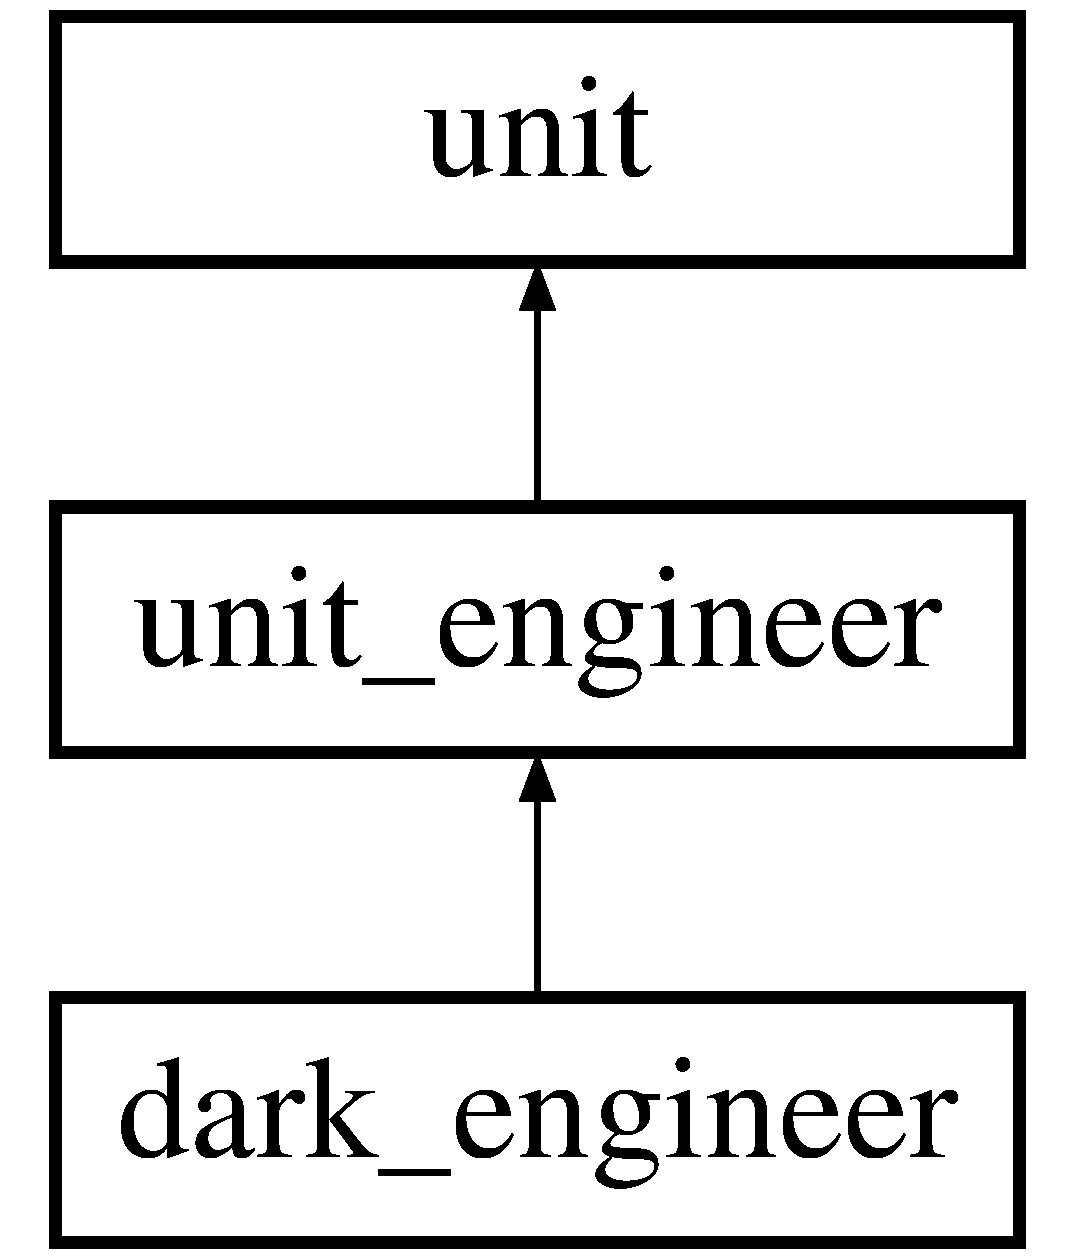
\includegraphics[height=3.000000cm]{classdark__engineer}
\end{center}
\end{figure}
\subsection*{Additional Inherited Members}


The documentation for this class was generated from the following file\+:\begin{DoxyCompactItemize}
\item 
dark\+\_\+fraction.\+h\end{DoxyCompactItemize}

\hypertarget{classdark__main__unit}{}\section{dark\+\_\+main\+\_\+unit Class Reference}
\label{classdark__main__unit}\index{dark\+\_\+main\+\_\+unit@{dark\+\_\+main\+\_\+unit}}
Inheritance diagram for dark\+\_\+main\+\_\+unit\+:\begin{figure}[H]
\begin{center}
\leavevmode
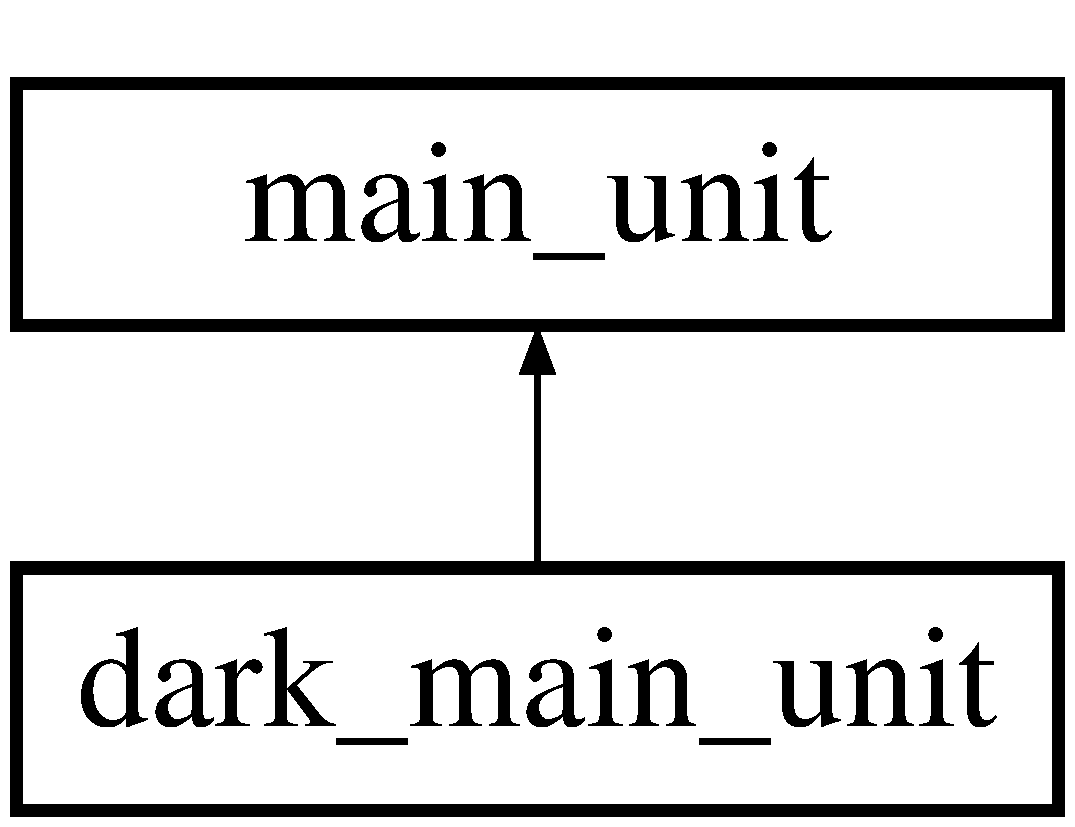
\includegraphics[height=2.000000cm]{classdark__main__unit}
\end{center}
\end{figure}
\subsection*{Additional Inherited Members}


The documentation for this class was generated from the following file\+:\begin{DoxyCompactItemize}
\item 
dark\+\_\+fraction.\+h\end{DoxyCompactItemize}

\hypertarget{classdark__solider}{}\section{dark\+\_\+solider Class Reference}
\label{classdark__solider}\index{dark\+\_\+solider@{dark\+\_\+solider}}
Inheritance diagram for dark\+\_\+solider\+:\begin{figure}[H]
\begin{center}
\leavevmode
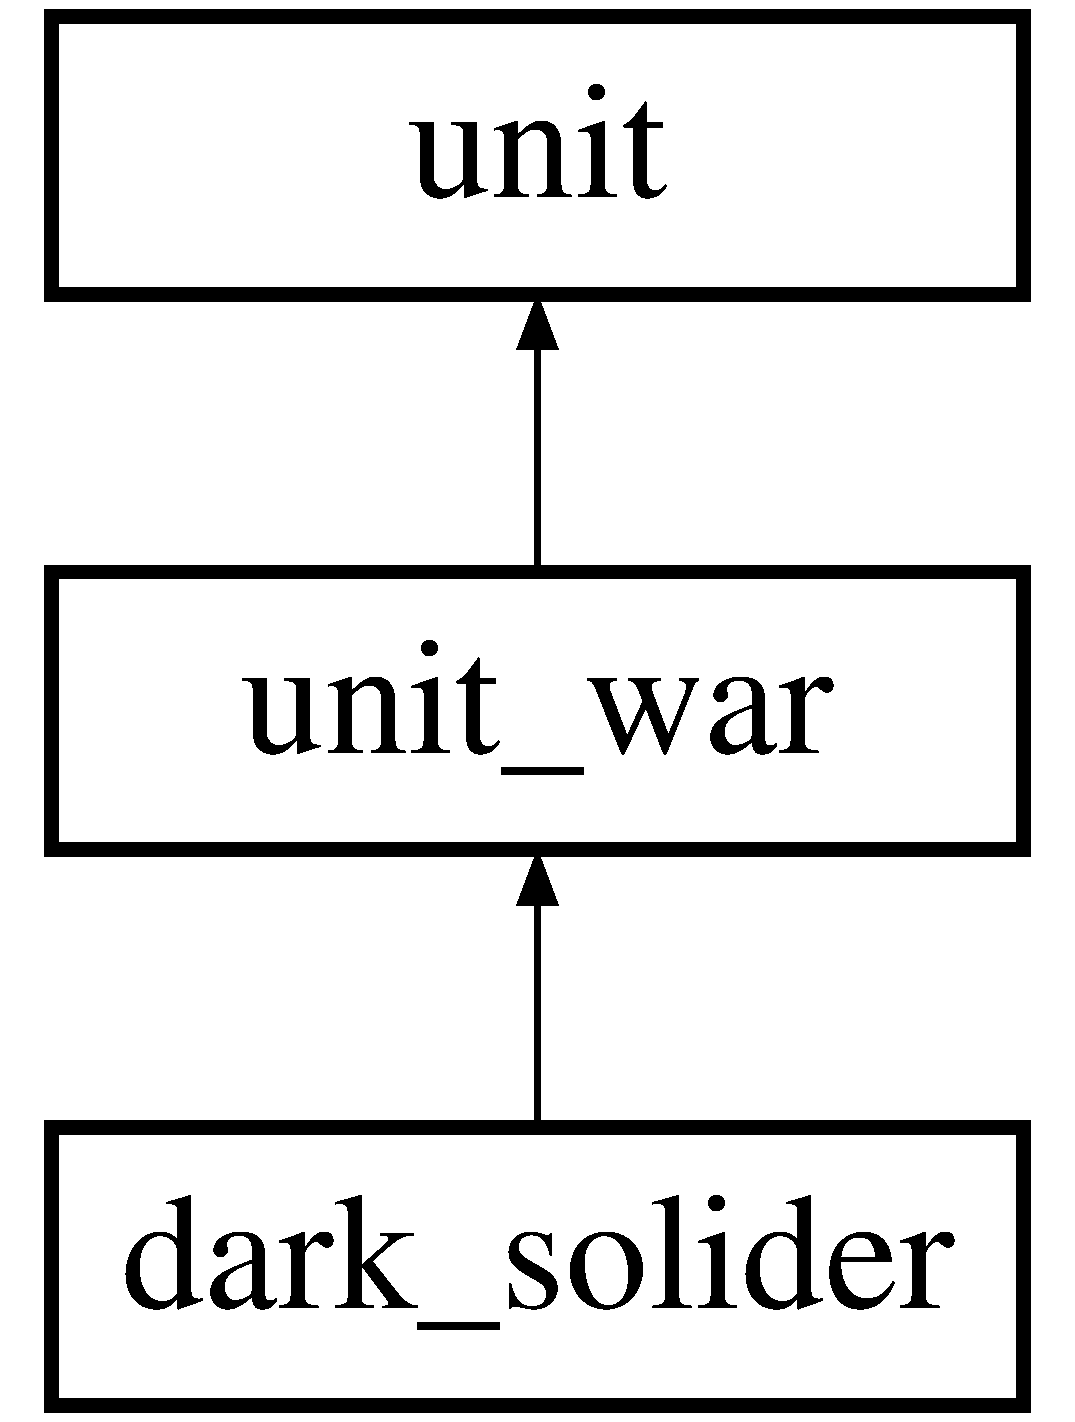
\includegraphics[height=3.000000cm]{classdark__solider}
\end{center}
\end{figure}
\subsection*{Public Member Functions}
\begin{DoxyCompactItemize}
\item 
\mbox{\Hypertarget{classdark__solider_a2d84b45483613bbf6203428246afcb9e}\label{classdark__solider_a2d84b45483613bbf6203428246afcb9e}} 
void {\bfseries get\+\_\+health} ()
\end{DoxyCompactItemize}
\subsection*{Additional Inherited Members}


The documentation for this class was generated from the following file\+:\begin{DoxyCompactItemize}
\item 
dark\+\_\+fraction.\+h\end{DoxyCompactItemize}

\hypertarget{classdark__surface__factory}{}\section{dark\+\_\+surface\+\_\+factory Class Reference}
\label{classdark__surface__factory}\index{dark\+\_\+surface\+\_\+factory@{dark\+\_\+surface\+\_\+factory}}
Inheritance diagram for dark\+\_\+surface\+\_\+factory\+:\begin{figure}[H]
\begin{center}
\leavevmode
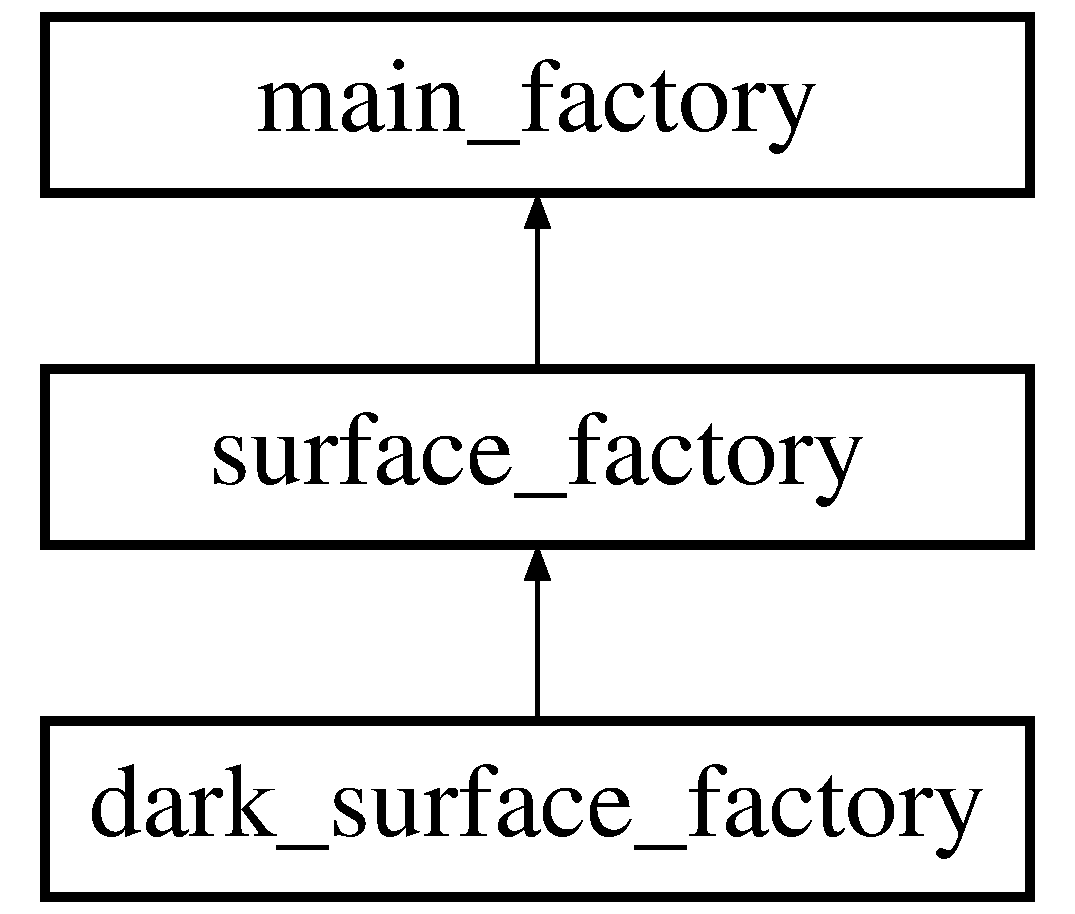
\includegraphics[height=3.000000cm]{classdark__surface__factory}
\end{center}
\end{figure}
\subsection*{Public Member Functions}
\begin{DoxyCompactItemize}
\item 
\mbox{\Hypertarget{classdark__surface__factory_a6b1b974f883da80bafcad845083e7a59}\label{classdark__surface__factory_a6b1b974f883da80bafcad845083e7a59}} 
\mbox{\hyperlink{classdark__solider}{dark\+\_\+solider}} $\ast$ {\bfseries build\+\_\+fast\+\_\+unit} () override
\item 
\mbox{\Hypertarget{classdark__surface__factory_a697d782a8318c85cd063c27a6b3a4434}\label{classdark__surface__factory_a697d782a8318c85cd063c27a6b3a4434}} 
\mbox{\hyperlink{classarmored__solider}{armored\+\_\+solider}} $\ast$ {\bfseries build\+\_\+armor\+\_\+unit} () override
\item 
\mbox{\Hypertarget{classdark__surface__factory_a91c92f8181a239e4eec7089cc77a1eb9}\label{classdark__surface__factory_a91c92f8181a239e4eec7089cc77a1eb9}} 
\mbox{\hyperlink{classfast__dark__scout}{fast\+\_\+dark\+\_\+scout}} $\ast$ {\bfseries build\+\_\+scout} () override
\item 
\mbox{\hyperlink{classdark__engineer}{dark\+\_\+engineer}} $\ast$ \mbox{\hyperlink{classdark__surface__factory_a70172395b97a039eed8e3ff193f9f6a6}{build\+\_\+engineer}} () override
\item 
\mbox{\Hypertarget{classdark__surface__factory_a20551ad19f38e2338fce0030d6ae4cb3}\label{classdark__surface__factory_a20551ad19f38e2338fce0030d6ae4cb3}} 
void {\bfseries ME} () override
\end{DoxyCompactItemize}
\subsection*{Additional Inherited Members}


\subsection{Member Function Documentation}
\mbox{\Hypertarget{classdark__surface__factory_a70172395b97a039eed8e3ff193f9f6a6}\label{classdark__surface__factory_a70172395b97a039eed8e3ff193f9f6a6}} 
\index{dark\+\_\+surface\+\_\+factory@{dark\+\_\+surface\+\_\+factory}!build\+\_\+engineer@{build\+\_\+engineer}}
\index{build\+\_\+engineer@{build\+\_\+engineer}!dark\+\_\+surface\+\_\+factory@{dark\+\_\+surface\+\_\+factory}}
\subsubsection{\texorpdfstring{build\+\_\+engineer()}{build\_engineer()}}
{\footnotesize\ttfamily \mbox{\hyperlink{classdark__engineer}{dark\+\_\+engineer}}$\ast$ dark\+\_\+surface\+\_\+factory\+::build\+\_\+engineer (\begin{DoxyParamCaption}{ }\end{DoxyParamCaption})\hspace{0.3cm}{\ttfamily [inline]}, {\ttfamily [override]}, {\ttfamily [virtual]}}

func to build an engineer \begin{DoxyReturn}{Returns}
new engineer 
\end{DoxyReturn}


Reimplemented from \mbox{\hyperlink{classmain__factory_ac970fe346638331722123f2bb240b590}{main\+\_\+factory}}.



The documentation for this class was generated from the following file\+:\begin{DoxyCompactItemize}
\item 
dark\+\_\+fraction.\+h\end{DoxyCompactItemize}

\hypertarget{classenergy}{}\section{energy Class Reference}
\label{classenergy}\index{energy@{energy}}


{\ttfamily \#include $<$main\+\_\+lib.\+h$>$}

\subsection*{Public Member Functions}
\begin{DoxyCompactItemize}
\item 
\mbox{\Hypertarget{classenergy_ae0727ccd1ee08fab458a5dda04ae94e2}\label{classenergy_ae0727ccd1ee08fab458a5dda04ae94e2}} 
{\bfseries energy} (const \mbox{\hyperlink{classenergy}{energy}} \&)=delete
\item 
\mbox{\Hypertarget{classenergy_a8133f32df6151974850d759ec56893ef}\label{classenergy_a8133f32df6151974850d759ec56893ef}} 
\mbox{\hyperlink{classenergy}{energy}} \& {\bfseries operator=} (\mbox{\hyperlink{classenergy}{energy}} \&)=delete
\end{DoxyCompactItemize}
\subsection*{Static Public Member Functions}
\begin{DoxyCompactItemize}
\item 
static void \mbox{\hyperlink{classenergy_a25298716dddd75c94bd034cc5f23033c}{increase\+\_\+energy}} (int energetic)
\item 
static void \mbox{\hyperlink{classenergy_a56d07f16cd58bbd82ff749fe010cbfd9}{decrease\+\_\+energy}} (int energy\+\_\+cost)
\end{DoxyCompactItemize}
\subsection*{Static Public Attributes}
\begin{DoxyCompactItemize}
\item 
\mbox{\Hypertarget{classenergy_a72cc46cb6eee3522c180d3f857f9fedc}\label{classenergy_a72cc46cb6eee3522c180d3f857f9fedc}} 
static int {\bfseries energy\+\_\+of\+\_\+player} = 0
\end{DoxyCompactItemize}


\subsection{Detailed Description}
brief Singletone class which contains energy of player 

\subsection{Member Function Documentation}
\mbox{\Hypertarget{classenergy_a56d07f16cd58bbd82ff749fe010cbfd9}\label{classenergy_a56d07f16cd58bbd82ff749fe010cbfd9}} 
\index{energy@{energy}!decrease\+\_\+energy@{decrease\+\_\+energy}}
\index{decrease\+\_\+energy@{decrease\+\_\+energy}!energy@{energy}}
\subsubsection{\texorpdfstring{decrease\+\_\+energy()}{decrease\_energy()}}
{\footnotesize\ttfamily static void energy\+::decrease\+\_\+energy (\begin{DoxyParamCaption}\item[{int}]{energy\+\_\+cost }\end{DoxyParamCaption})\hspace{0.3cm}{\ttfamily [inline]}, {\ttfamily [static]}}

brief decreases energy of player 
\begin{DoxyParams}{Parameters}
{\em energy\+\_\+cost} & \\
\hline
\end{DoxyParams}
\mbox{\Hypertarget{classenergy_a25298716dddd75c94bd034cc5f23033c}\label{classenergy_a25298716dddd75c94bd034cc5f23033c}} 
\index{energy@{energy}!increase\+\_\+energy@{increase\+\_\+energy}}
\index{increase\+\_\+energy@{increase\+\_\+energy}!energy@{energy}}
\subsubsection{\texorpdfstring{increase\+\_\+energy()}{increase\_energy()}}
{\footnotesize\ttfamily static void energy\+::increase\+\_\+energy (\begin{DoxyParamCaption}\item[{int}]{energetic }\end{DoxyParamCaption})\hspace{0.3cm}{\ttfamily [inline]}, {\ttfamily [static]}}

brief increases eneregy of player 
\begin{DoxyParams}{Parameters}
{\em energetic} & \\
\hline
\end{DoxyParams}


The documentation for this class was generated from the following file\+:\begin{DoxyCompactItemize}
\item 
main\+\_\+lib.\+h\end{DoxyCompactItemize}

\hypertarget{classextra__unit__builder}{}\section{extra\+\_\+unit\+\_\+builder Class Reference}
\label{classextra__unit__builder}\index{extra\+\_\+unit\+\_\+builder@{extra\+\_\+unit\+\_\+builder}}


{\ttfamily \#include $<$main\+\_\+lib.\+h$>$}

Inheritance diagram for extra\+\_\+unit\+\_\+builder\+:\begin{figure}[H]
\begin{center}
\leavevmode
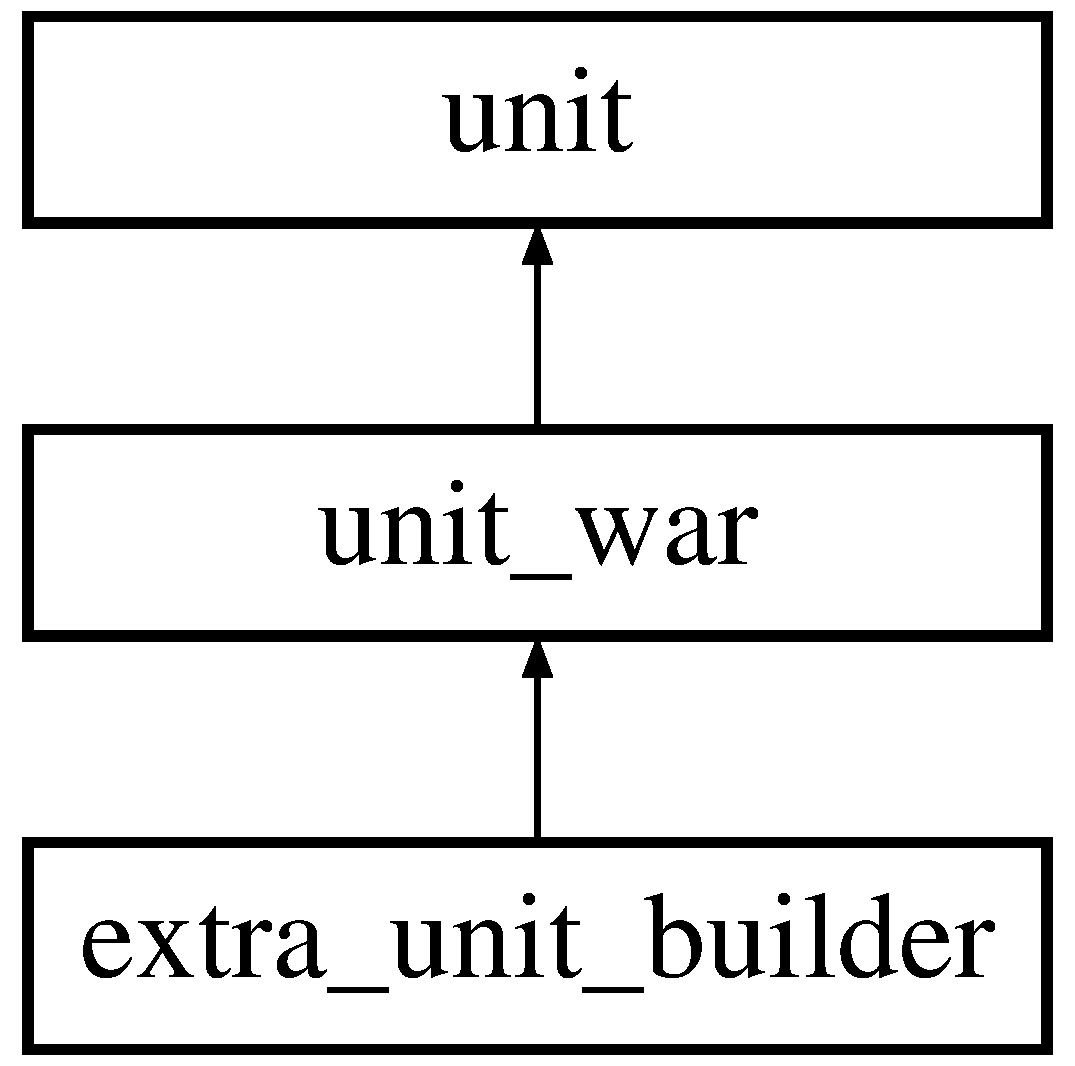
\includegraphics[height=3.000000cm]{classextra__unit__builder}
\end{center}
\end{figure}
\subsection*{Public Member Functions}
\begin{DoxyCompactItemize}
\item 
\mbox{\Hypertarget{classextra__unit__builder_a881bf623a6795bd39fc1e490f74fc794}\label{classextra__unit__builder_a881bf623a6795bd39fc1e490f74fc794}} 
void {\bfseries set\+\_\+air\+\_\+deff} (int damage)
\item 
void \mbox{\hyperlink{classextra__unit__builder_aa95d6dcfba85a06592d6725baebd51cc}{set\+\_\+speed}} (int \+\_\+speed) override
\item 
void \mbox{\hyperlink{classextra__unit__builder_a7471f05c65d3f2c230c405ec0bcdaa7d}{set\+\_\+health}} (int \+\_\+health) override
\item 
void \mbox{\hyperlink{classextra__unit__builder_a98602fd267039102bd6b431bdf5b658d}{set\+\_\+power}} (int \+\_\+power) override
\item 
const int \mbox{\hyperlink{classextra__unit__builder_a84ce334361c5acd1a59775a74fabde86}{get\+\_\+cost}} () override
\end{DoxyCompactItemize}
\subsection*{Additional Inherited Members}


\subsection{Detailed Description}
brief special unit that u can build with your own characteristics 

\subsection{Member Function Documentation}
\mbox{\Hypertarget{classextra__unit__builder_a84ce334361c5acd1a59775a74fabde86}\label{classextra__unit__builder_a84ce334361c5acd1a59775a74fabde86}} 
\index{extra\+\_\+unit\+\_\+builder@{extra\+\_\+unit\+\_\+builder}!get\+\_\+cost@{get\+\_\+cost}}
\index{get\+\_\+cost@{get\+\_\+cost}!extra\+\_\+unit\+\_\+builder@{extra\+\_\+unit\+\_\+builder}}
\subsubsection{\texorpdfstring{get\+\_\+cost()}{get\_cost()}}
{\footnotesize\ttfamily const int extra\+\_\+unit\+\_\+builder\+::get\+\_\+cost (\begin{DoxyParamCaption}{ }\end{DoxyParamCaption})\hspace{0.3cm}{\ttfamily [inline]}, {\ttfamily [override]}, {\ttfamily [virtual]}}

func that returns cost of the unit \begin{DoxyReturn}{Returns}
cost of the unit 
\end{DoxyReturn}


Reimplemented from \mbox{\hyperlink{classunit_a817ef860467c21c378deb39f738c33e0}{unit}}.

\mbox{\Hypertarget{classextra__unit__builder_a7471f05c65d3f2c230c405ec0bcdaa7d}\label{classextra__unit__builder_a7471f05c65d3f2c230c405ec0bcdaa7d}} 
\index{extra\+\_\+unit\+\_\+builder@{extra\+\_\+unit\+\_\+builder}!set\+\_\+health@{set\+\_\+health}}
\index{set\+\_\+health@{set\+\_\+health}!extra\+\_\+unit\+\_\+builder@{extra\+\_\+unit\+\_\+builder}}
\subsubsection{\texorpdfstring{set\+\_\+health()}{set\_health()}}
{\footnotesize\ttfamily void extra\+\_\+unit\+\_\+builder\+::set\+\_\+health (\begin{DoxyParamCaption}\item[{int}]{c }\end{DoxyParamCaption})\hspace{0.3cm}{\ttfamily [inline]}, {\ttfamily [override]}, {\ttfamily [virtual]}}

brief sets health of unit 
\begin{DoxyParams}{Parameters}
{\em c} & \\
\hline
\end{DoxyParams}


Reimplemented from \mbox{\hyperlink{classunit_a1dabc406074919750b1c606496e8e42d}{unit}}.

\mbox{\Hypertarget{classextra__unit__builder_a98602fd267039102bd6b431bdf5b658d}\label{classextra__unit__builder_a98602fd267039102bd6b431bdf5b658d}} 
\index{extra\+\_\+unit\+\_\+builder@{extra\+\_\+unit\+\_\+builder}!set\+\_\+power@{set\+\_\+power}}
\index{set\+\_\+power@{set\+\_\+power}!extra\+\_\+unit\+\_\+builder@{extra\+\_\+unit\+\_\+builder}}
\subsubsection{\texorpdfstring{set\+\_\+power()}{set\_power()}}
{\footnotesize\ttfamily void extra\+\_\+unit\+\_\+builder\+::set\+\_\+power (\begin{DoxyParamCaption}\item[{int}]{b }\end{DoxyParamCaption})\hspace{0.3cm}{\ttfamily [inline]}, {\ttfamily [override]}, {\ttfamily [virtual]}}

brief sets power of unit 
\begin{DoxyParams}{Parameters}
{\em b} & \\
\hline
\end{DoxyParams}


Reimplemented from \mbox{\hyperlink{classunit__war_a8ea09eb3e352d5a3b2d7611ac78124a2}{unit\+\_\+war}}.

\mbox{\Hypertarget{classextra__unit__builder_aa95d6dcfba85a06592d6725baebd51cc}\label{classextra__unit__builder_aa95d6dcfba85a06592d6725baebd51cc}} 
\index{extra\+\_\+unit\+\_\+builder@{extra\+\_\+unit\+\_\+builder}!set\+\_\+speed@{set\+\_\+speed}}
\index{set\+\_\+speed@{set\+\_\+speed}!extra\+\_\+unit\+\_\+builder@{extra\+\_\+unit\+\_\+builder}}
\subsubsection{\texorpdfstring{set\+\_\+speed()}{set\_speed()}}
{\footnotesize\ttfamily void extra\+\_\+unit\+\_\+builder\+::set\+\_\+speed (\begin{DoxyParamCaption}\item[{int}]{a }\end{DoxyParamCaption})\hspace{0.3cm}{\ttfamily [inline]}, {\ttfamily [override]}, {\ttfamily [virtual]}}

brief sets speed of unit 
\begin{DoxyParams}{Parameters}
{\em a} & \\
\hline
\end{DoxyParams}


Reimplemented from \mbox{\hyperlink{classunit_a3b2dbfe9c1daaf2b8ef6b604d7803dc2}{unit}}.



The documentation for this class was generated from the following file\+:\begin{DoxyCompactItemize}
\item 
main\+\_\+lib.\+h\end{DoxyCompactItemize}

\hypertarget{classfast__dark__scout}{}\section{fast\+\_\+dark\+\_\+scout Class Reference}
\label{classfast__dark__scout}\index{fast\+\_\+dark\+\_\+scout@{fast\+\_\+dark\+\_\+scout}}
Inheritance diagram for fast\+\_\+dark\+\_\+scout\+:\begin{figure}[H]
\begin{center}
\leavevmode
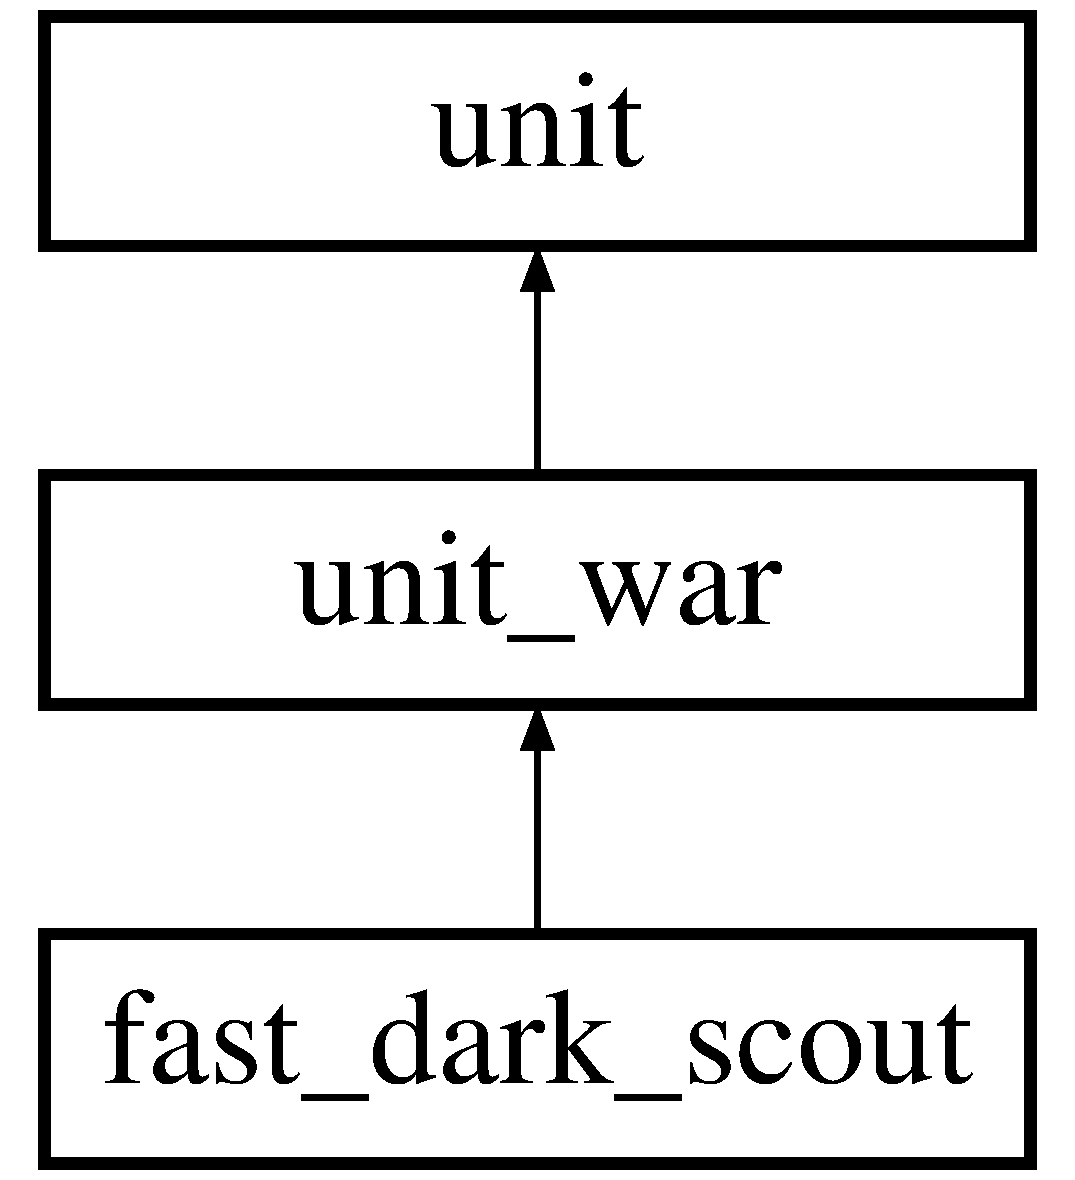
\includegraphics[height=3.000000cm]{classfast__dark__scout}
\end{center}
\end{figure}
\subsection*{Additional Inherited Members}


The documentation for this class was generated from the following file\+:\begin{DoxyCompactItemize}
\item 
dark\+\_\+fraction.\+h\end{DoxyCompactItemize}

\hypertarget{classfast__scout}{}\section{fast\+\_\+scout Class Reference}
\label{classfast__scout}\index{fast\+\_\+scout@{fast\+\_\+scout}}
Inheritance diagram for fast\+\_\+scout\+:\begin{figure}[H]
\begin{center}
\leavevmode
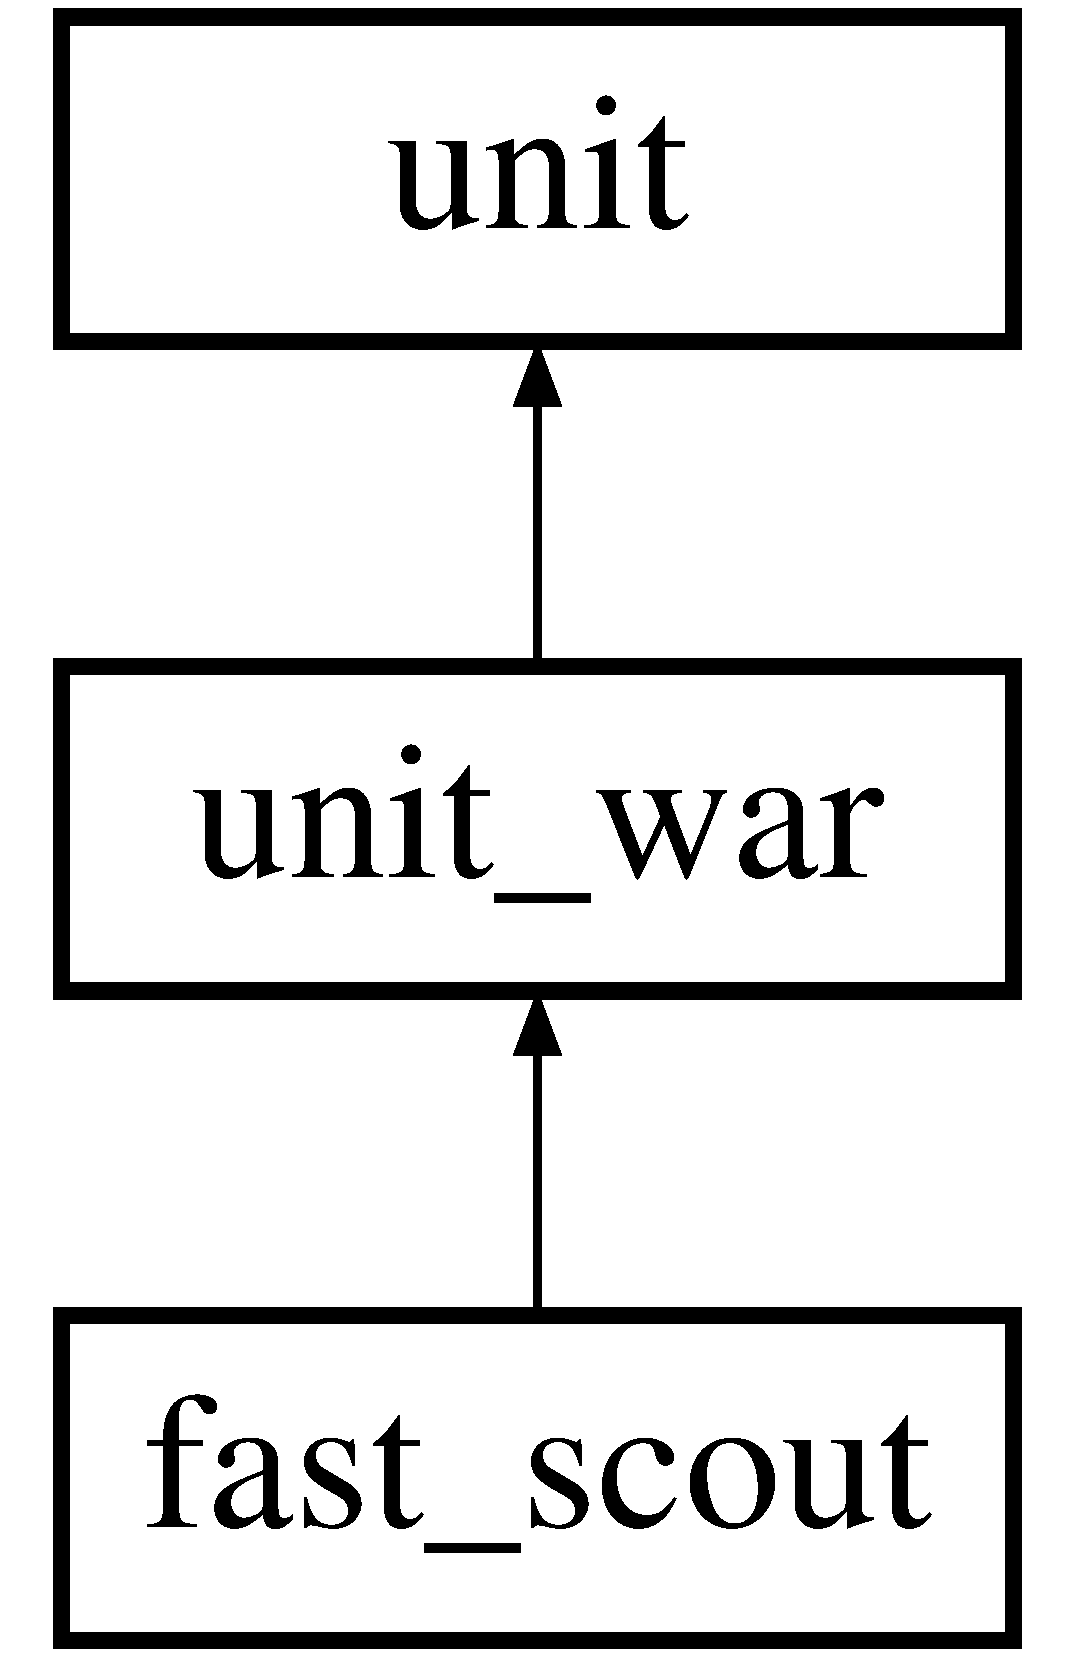
\includegraphics[height=3.000000cm]{classfast__scout}
\end{center}
\end{figure}
\subsection*{Additional Inherited Members}


The documentation for this class was generated from the following file\+:\begin{DoxyCompactItemize}
\item 
human\+\_\+tree.\+h\end{DoxyCompactItemize}

\hypertarget{classflying__unit}{}\section{flying\+\_\+unit Class Reference}
\label{classflying__unit}\index{flying\+\_\+unit@{flying\+\_\+unit}}


{\ttfamily \#include $<$main\+\_\+lib.\+h$>$}

Inheritance diagram for flying\+\_\+unit\+:\begin{figure}[H]
\begin{center}
\leavevmode
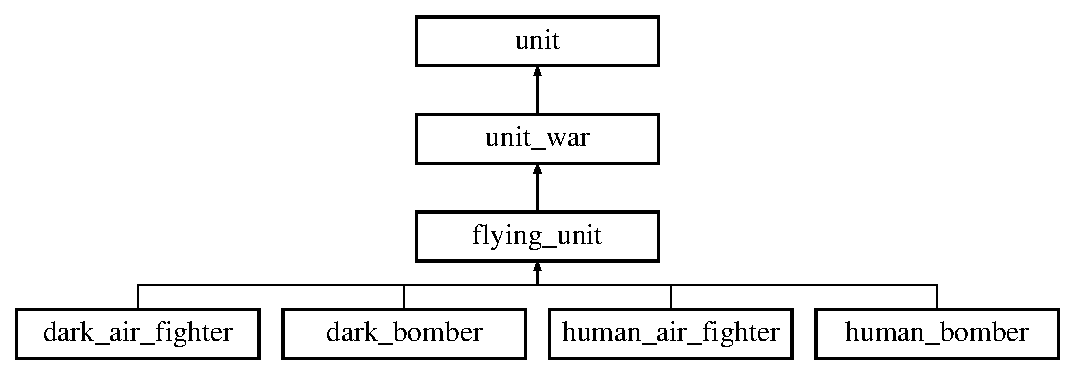
\includegraphics[height=4.000000cm]{classflying__unit}
\end{center}
\end{figure}
\subsection*{Public Member Functions}
\begin{DoxyCompactItemize}
\item 
const int \mbox{\hyperlink{classflying__unit_a95333465a28d47bc5d50427fd3e2cef4}{get\+\_\+power}} () override
\item 
const int \mbox{\hyperlink{classflying__unit_a47dbbf3832a5b5e8f5365d87cdbfddab}{get\+\_\+air\+\_\+deffence}} () override
\end{DoxyCompactItemize}
\subsection*{Protected Member Functions}
\begin{DoxyCompactItemize}
\item 
void \mbox{\hyperlink{classflying__unit_a2b220aabd9faa894c96bb13e03b5a9f5}{set\+\_\+air\+\_\+attack}} (int damage)
\item 
void \mbox{\hyperlink{classflying__unit_a751bb2f477f2904a7de06218159c1dff}{set\+\_\+ground\+\_\+attack}} (int damage)
\end{DoxyCompactItemize}
\subsection*{Additional Inherited Members}


\subsection{Detailed Description}
brief special unit that can fly 

\subsection{Member Function Documentation}
\mbox{\Hypertarget{classflying__unit_a47dbbf3832a5b5e8f5365d87cdbfddab}\label{classflying__unit_a47dbbf3832a5b5e8f5365d87cdbfddab}} 
\index{flying\+\_\+unit@{flying\+\_\+unit}!get\+\_\+air\+\_\+deffence@{get\+\_\+air\+\_\+deffence}}
\index{get\+\_\+air\+\_\+deffence@{get\+\_\+air\+\_\+deffence}!flying\+\_\+unit@{flying\+\_\+unit}}
\subsubsection{\texorpdfstring{get\+\_\+air\+\_\+deffence()}{get\_air\_deffence()}}
{\footnotesize\ttfamily const int flying\+\_\+unit\+::get\+\_\+air\+\_\+deffence (\begin{DoxyParamCaption}{ }\end{DoxyParamCaption})\hspace{0.3cm}{\ttfamily [inline]}, {\ttfamily [override]}, {\ttfamily [virtual]}}

brief air\+\_\+defence power info \begin{DoxyReturn}{Returns}
air defence power 
\end{DoxyReturn}


Reimplemented from \mbox{\hyperlink{classunit__war_af26f2da420a828230a329339bc9ef805}{unit\+\_\+war}}.

\mbox{\Hypertarget{classflying__unit_a95333465a28d47bc5d50427fd3e2cef4}\label{classflying__unit_a95333465a28d47bc5d50427fd3e2cef4}} 
\index{flying\+\_\+unit@{flying\+\_\+unit}!get\+\_\+power@{get\+\_\+power}}
\index{get\+\_\+power@{get\+\_\+power}!flying\+\_\+unit@{flying\+\_\+unit}}
\subsubsection{\texorpdfstring{get\+\_\+power()}{get\_power()}}
{\footnotesize\ttfamily const int flying\+\_\+unit\+::get\+\_\+power (\begin{DoxyParamCaption}{ }\end{DoxyParamCaption})\hspace{0.3cm}{\ttfamily [inline]}, {\ttfamily [override]}, {\ttfamily [virtual]}}

brief returns power of unit \begin{DoxyReturn}{Returns}
power of unit 
\end{DoxyReturn}


Reimplemented from \mbox{\hyperlink{classunit__war_adea1fced490739cf8b7a6e49ec90cf59}{unit\+\_\+war}}.

\mbox{\Hypertarget{classflying__unit_a2b220aabd9faa894c96bb13e03b5a9f5}\label{classflying__unit_a2b220aabd9faa894c96bb13e03b5a9f5}} 
\index{flying\+\_\+unit@{flying\+\_\+unit}!set\+\_\+air\+\_\+attack@{set\+\_\+air\+\_\+attack}}
\index{set\+\_\+air\+\_\+attack@{set\+\_\+air\+\_\+attack}!flying\+\_\+unit@{flying\+\_\+unit}}
\subsubsection{\texorpdfstring{set\+\_\+air\+\_\+attack()}{set\_air\_attack()}}
{\footnotesize\ttfamily void flying\+\_\+unit\+::set\+\_\+air\+\_\+attack (\begin{DoxyParamCaption}\item[{int}]{damage }\end{DoxyParamCaption})\hspace{0.3cm}{\ttfamily [inline]}, {\ttfamily [protected]}}

brief sets attack in air 
\begin{DoxyParams}{Parameters}
{\em damage} & \\
\hline
\end{DoxyParams}
\mbox{\Hypertarget{classflying__unit_a751bb2f477f2904a7de06218159c1dff}\label{classflying__unit_a751bb2f477f2904a7de06218159c1dff}} 
\index{flying\+\_\+unit@{flying\+\_\+unit}!set\+\_\+ground\+\_\+attack@{set\+\_\+ground\+\_\+attack}}
\index{set\+\_\+ground\+\_\+attack@{set\+\_\+ground\+\_\+attack}!flying\+\_\+unit@{flying\+\_\+unit}}
\subsubsection{\texorpdfstring{set\+\_\+ground\+\_\+attack()}{set\_ground\_attack()}}
{\footnotesize\ttfamily void flying\+\_\+unit\+::set\+\_\+ground\+\_\+attack (\begin{DoxyParamCaption}\item[{int}]{damage }\end{DoxyParamCaption})\hspace{0.3cm}{\ttfamily [inline]}, {\ttfamily [protected]}}

brief sets attack of ground 
\begin{DoxyParams}{Parameters}
{\em damage} & \\
\hline
\end{DoxyParams}


The documentation for this class was generated from the following file\+:\begin{DoxyCompactItemize}
\item 
main\+\_\+lib.\+h\end{DoxyCompactItemize}

\hypertarget{classgenerator__of__energy}{}\section{generator\+\_\+of\+\_\+energy Class Reference}
\label{classgenerator__of__energy}\index{generator\+\_\+of\+\_\+energy@{generator\+\_\+of\+\_\+energy}}


{\ttfamily \#include $<$main\+\_\+lib.\+h$>$}

\subsection*{Public Attributes}
\begin{DoxyCompactItemize}
\item 
\mbox{\Hypertarget{classgenerator__of__energy_ad193a7482acaa051e7d4afa63e51c06a}\label{classgenerator__of__energy_ad193a7482acaa051e7d4afa63e51c06a}} 
int {\bfseries energy\+\_\+per\+\_\+second}
\end{DoxyCompactItemize}
\subsection*{Static Public Attributes}
\begin{DoxyCompactItemize}
\item 
\mbox{\Hypertarget{classgenerator__of__energy_a5b440fb547e182d49fe94a50b5b86896}\label{classgenerator__of__energy_a5b440fb547e182d49fe94a50b5b86896}} 
static int {\bfseries how\+\_\+many} = 0
\end{DoxyCompactItemize}


\subsection{Detailed Description}
brief class for energy generator 

The documentation for this class was generated from the following file\+:\begin{DoxyCompactItemize}
\item 
main\+\_\+lib.\+h\end{DoxyCompactItemize}

\hypertarget{classhuman__air__factory}{}\section{human\+\_\+air\+\_\+factory Class Reference}
\label{classhuman__air__factory}\index{human\+\_\+air\+\_\+factory@{human\+\_\+air\+\_\+factory}}
Inheritance diagram for human\+\_\+air\+\_\+factory\+:\begin{figure}[H]
\begin{center}
\leavevmode
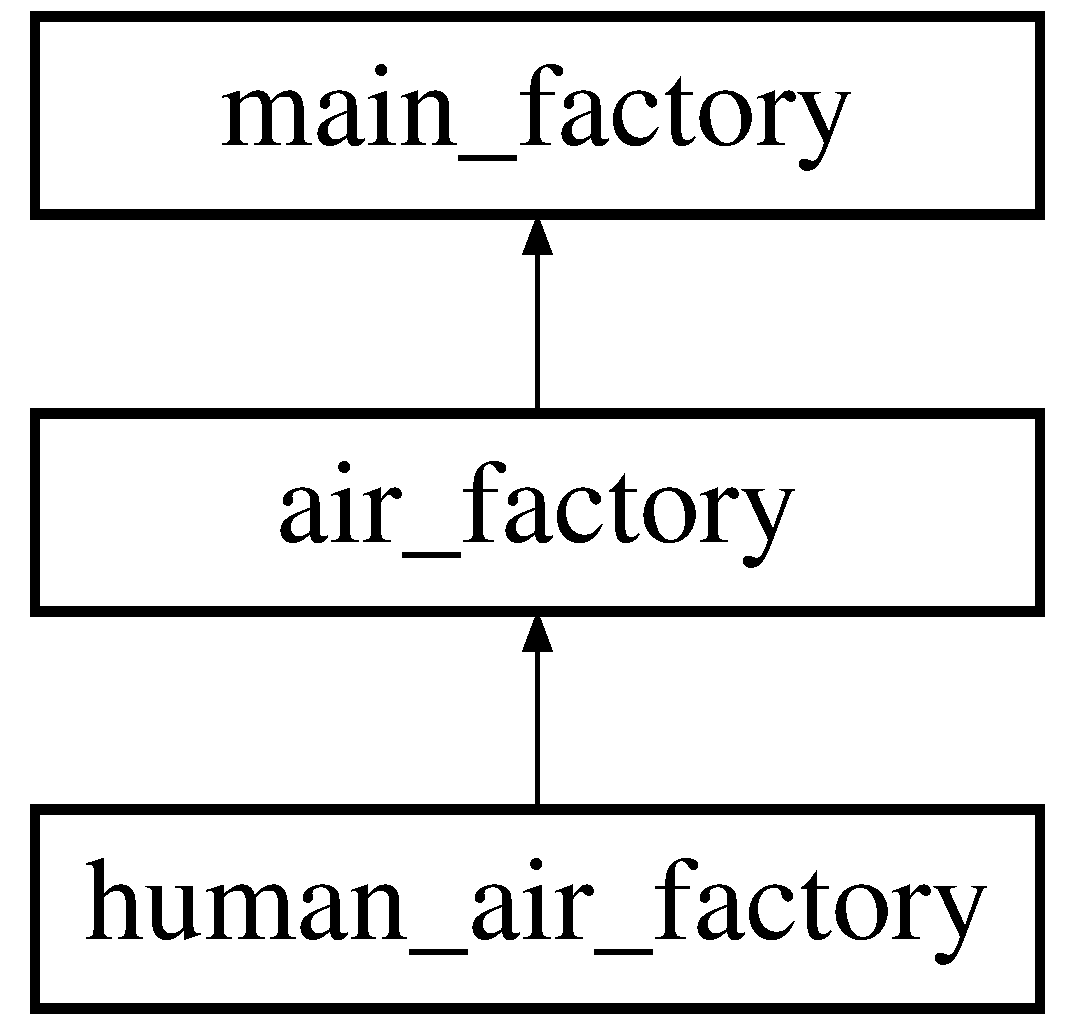
\includegraphics[height=3.000000cm]{classhuman__air__factory}
\end{center}
\end{figure}
\subsection*{Public Member Functions}
\begin{DoxyCompactItemize}
\item 
\mbox{\Hypertarget{classhuman__air__factory_a3d60a824005f82e14becc37a4c62873f}\label{classhuman__air__factory_a3d60a824005f82e14becc37a4c62873f}} 
\mbox{\hyperlink{classhuman__bomber}{human\+\_\+bomber}} $\ast$ {\bfseries build\+\_\+bomber} () override
\item 
\mbox{\Hypertarget{classhuman__air__factory_ab773ad15d45d82eefcae174205382ef6}\label{classhuman__air__factory_ab773ad15d45d82eefcae174205382ef6}} 
\mbox{\hyperlink{classhuman__air__fighter}{human\+\_\+air\+\_\+fighter}} $\ast$ {\bfseries build\+\_\+fighter} () override
\item 
\mbox{\hyperlink{classhuman__engineer}{human\+\_\+engineer}} $\ast$ \mbox{\hyperlink{classhuman__air__factory_a34707f920a66afe9af4d5b0ecef8b2a7}{build\+\_\+engineer}} () override
\end{DoxyCompactItemize}
\subsection*{Additional Inherited Members}


\subsection{Member Function Documentation}
\mbox{\Hypertarget{classhuman__air__factory_a34707f920a66afe9af4d5b0ecef8b2a7}\label{classhuman__air__factory_a34707f920a66afe9af4d5b0ecef8b2a7}} 
\index{human\+\_\+air\+\_\+factory@{human\+\_\+air\+\_\+factory}!build\+\_\+engineer@{build\+\_\+engineer}}
\index{build\+\_\+engineer@{build\+\_\+engineer}!human\+\_\+air\+\_\+factory@{human\+\_\+air\+\_\+factory}}
\subsubsection{\texorpdfstring{build\+\_\+engineer()}{build\_engineer()}}
{\footnotesize\ttfamily \mbox{\hyperlink{classhuman__engineer}{human\+\_\+engineer}}$\ast$ human\+\_\+air\+\_\+factory\+::build\+\_\+engineer (\begin{DoxyParamCaption}{ }\end{DoxyParamCaption})\hspace{0.3cm}{\ttfamily [inline]}, {\ttfamily [override]}, {\ttfamily [virtual]}}

func to build an engineer \begin{DoxyReturn}{Returns}
new engineer 
\end{DoxyReturn}


Reimplemented from \mbox{\hyperlink{classmain__factory_ac970fe346638331722123f2bb240b590}{main\+\_\+factory}}.



The documentation for this class was generated from the following file\+:\begin{DoxyCompactItemize}
\item 
human\+\_\+tree.\+h\end{DoxyCompactItemize}

\hypertarget{classhuman__air__fighter}{}\section{human\+\_\+air\+\_\+fighter Class Reference}
\label{classhuman__air__fighter}\index{human\+\_\+air\+\_\+fighter@{human\+\_\+air\+\_\+fighter}}
Inheritance diagram for human\+\_\+air\+\_\+fighter\+:\begin{figure}[H]
\begin{center}
\leavevmode
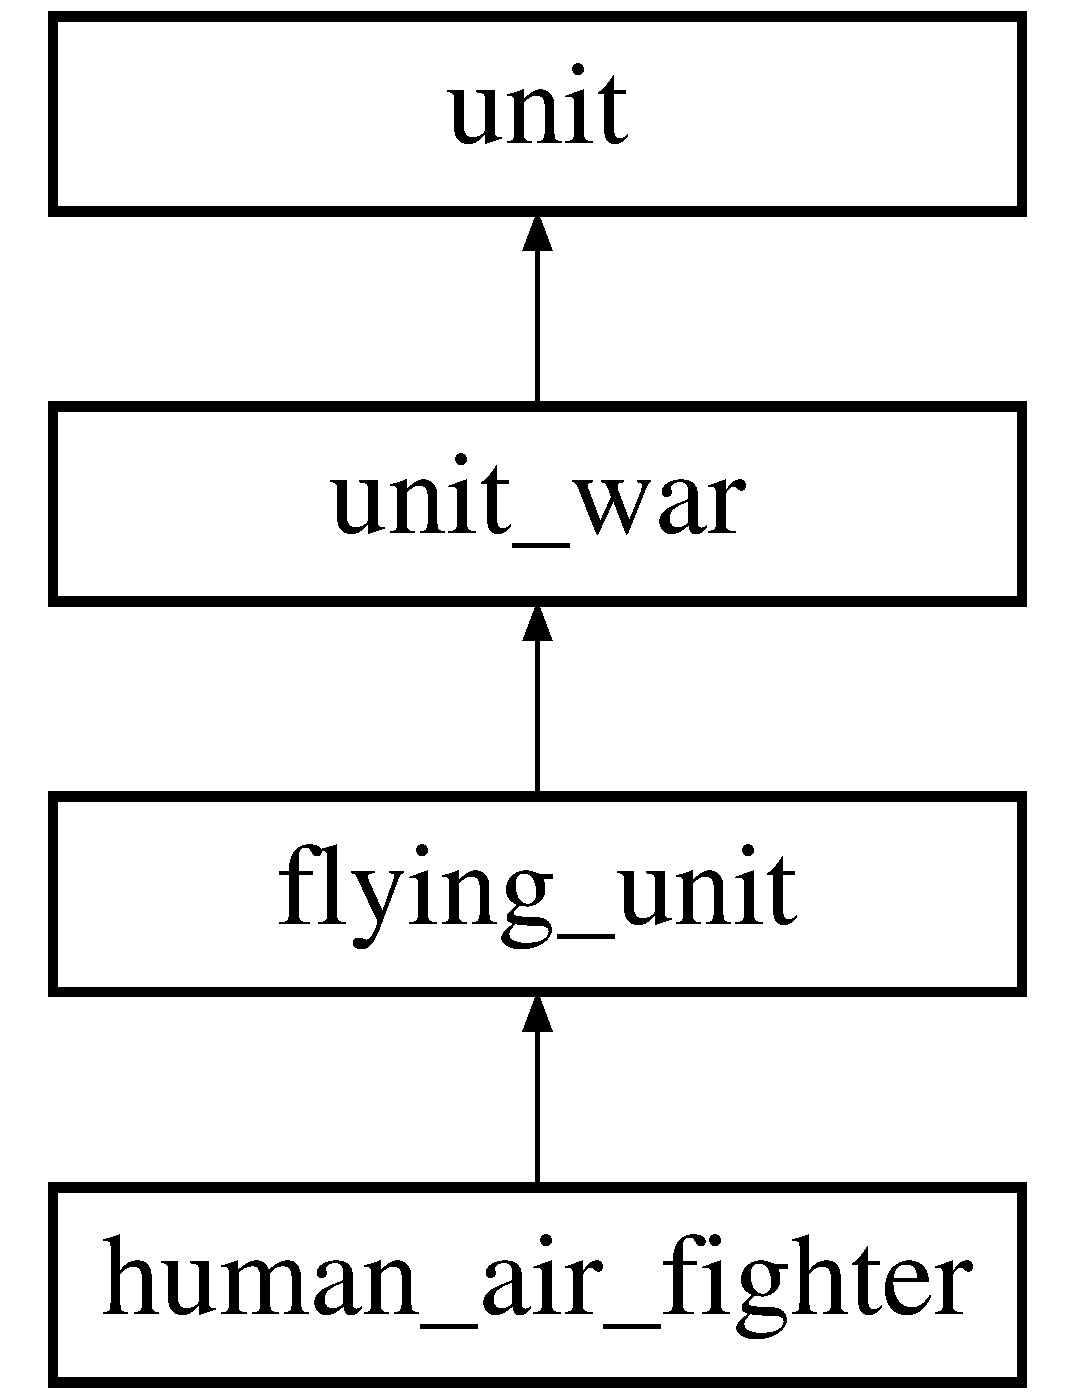
\includegraphics[height=4.000000cm]{classhuman__air__fighter}
\end{center}
\end{figure}
\subsection*{Additional Inherited Members}


The documentation for this class was generated from the following file\+:\begin{DoxyCompactItemize}
\item 
human\+\_\+tree.\+h\end{DoxyCompactItemize}

\hypertarget{classhuman__bomber}{}\section{human\+\_\+bomber Class Reference}
\label{classhuman__bomber}\index{human\+\_\+bomber@{human\+\_\+bomber}}
Inheritance diagram for human\+\_\+bomber\+:\begin{figure}[H]
\begin{center}
\leavevmode
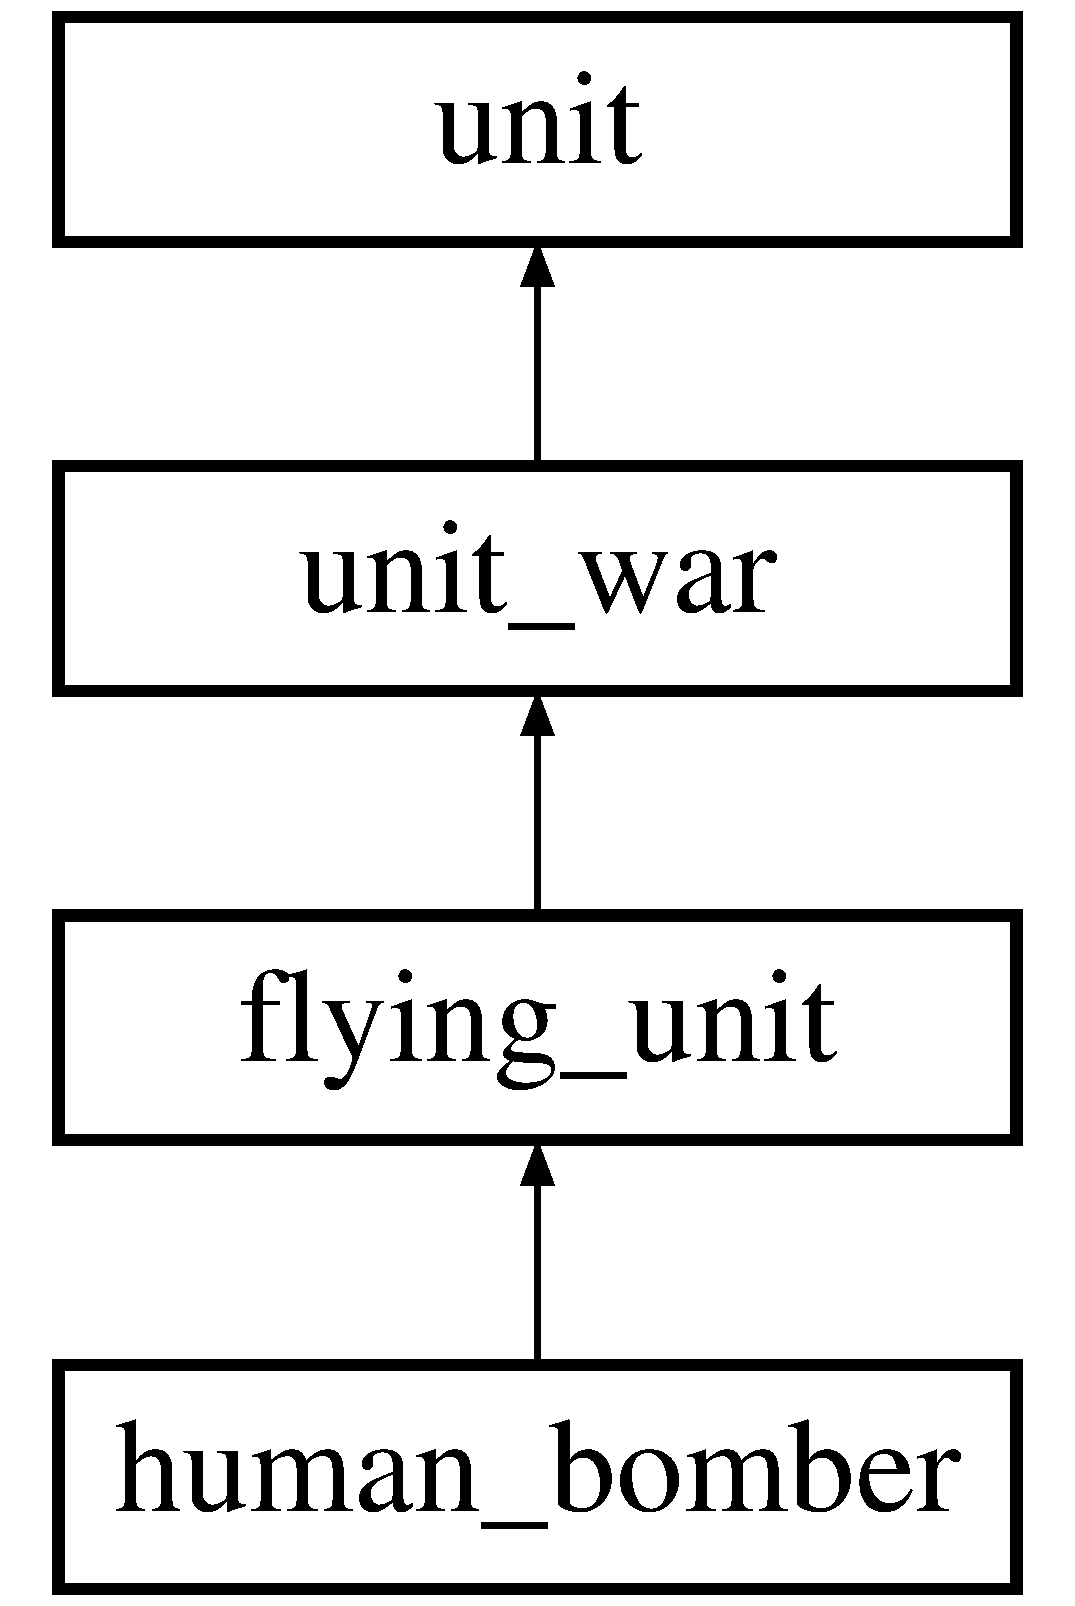
\includegraphics[height=4.000000cm]{classhuman__bomber}
\end{center}
\end{figure}
\subsection*{Additional Inherited Members}


The documentation for this class was generated from the following file\+:\begin{DoxyCompactItemize}
\item 
human\+\_\+tree.\+h\end{DoxyCompactItemize}

\hypertarget{classhuman__engineer}{}\section{human\+\_\+engineer Class Reference}
\label{classhuman__engineer}\index{human\+\_\+engineer@{human\+\_\+engineer}}
Inheritance diagram for human\+\_\+engineer\+:\begin{figure}[H]
\begin{center}
\leavevmode
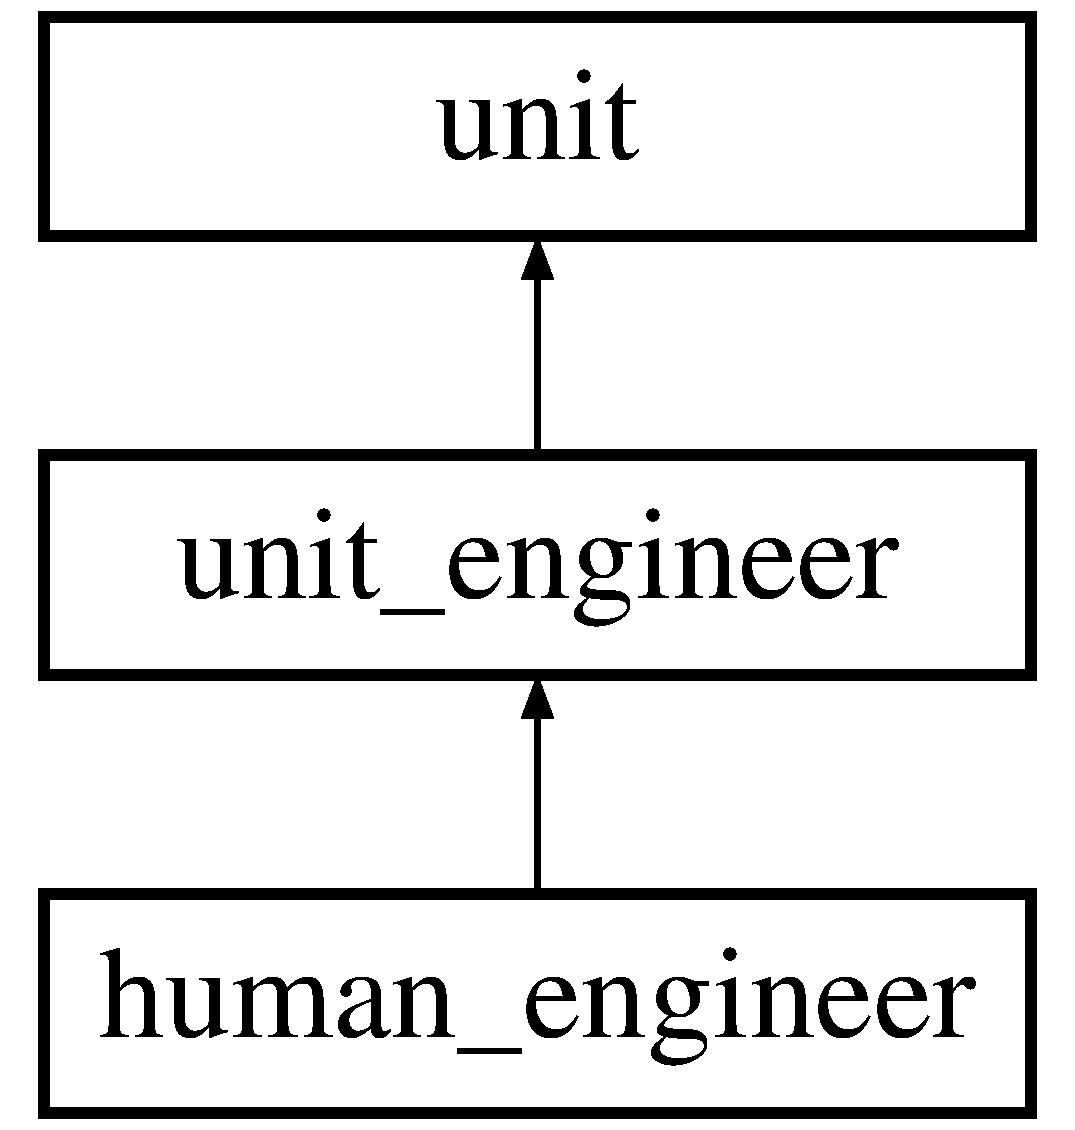
\includegraphics[height=3.000000cm]{classhuman__engineer}
\end{center}
\end{figure}
\subsection*{Additional Inherited Members}


The documentation for this class was generated from the following file\+:\begin{DoxyCompactItemize}
\item 
human\+\_\+tree.\+h\end{DoxyCompactItemize}

\hypertarget{classhuman__main__unit}{}\section{human\+\_\+main\+\_\+unit Class Reference}
\label{classhuman__main__unit}\index{human\+\_\+main\+\_\+unit@{human\+\_\+main\+\_\+unit}}
Inheritance diagram for human\+\_\+main\+\_\+unit\+:\begin{figure}[H]
\begin{center}
\leavevmode
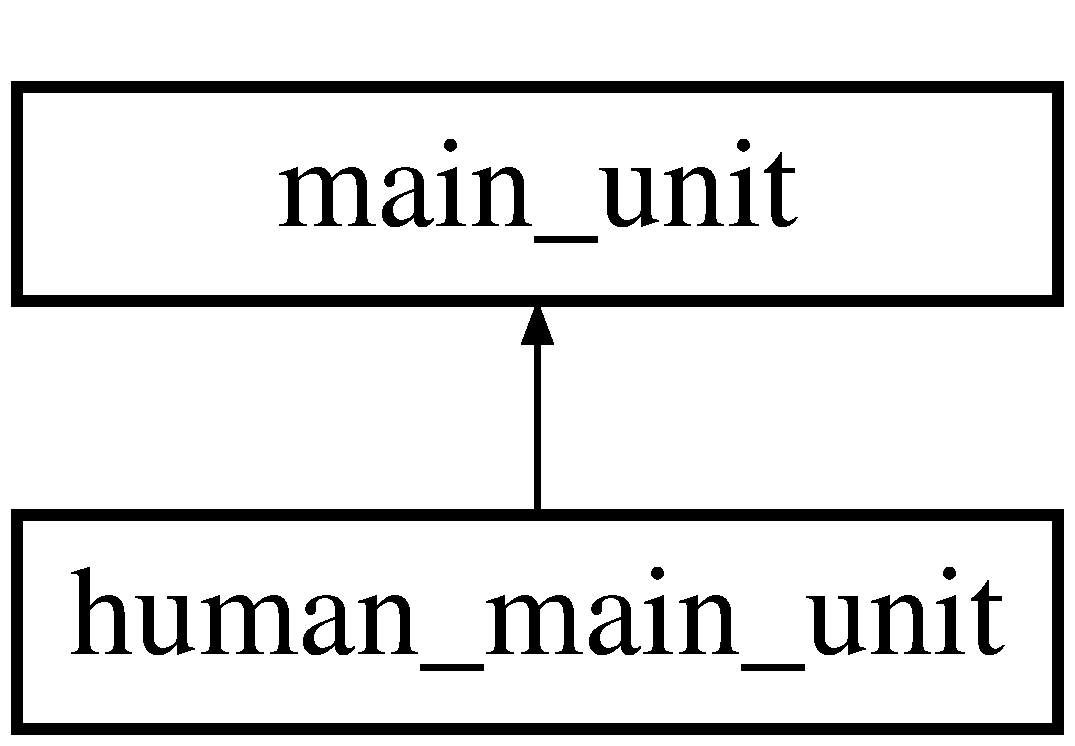
\includegraphics[height=2.000000cm]{classhuman__main__unit}
\end{center}
\end{figure}
\subsection*{Additional Inherited Members}


The documentation for this class was generated from the following file\+:\begin{DoxyCompactItemize}
\item 
human\+\_\+tree.\+h\end{DoxyCompactItemize}

\hypertarget{classhuman__surface__factory}{}\section{human\+\_\+surface\+\_\+factory Class Reference}
\label{classhuman__surface__factory}\index{human\+\_\+surface\+\_\+factory@{human\+\_\+surface\+\_\+factory}}
Inheritance diagram for human\+\_\+surface\+\_\+factory\+:\begin{figure}[H]
\begin{center}
\leavevmode
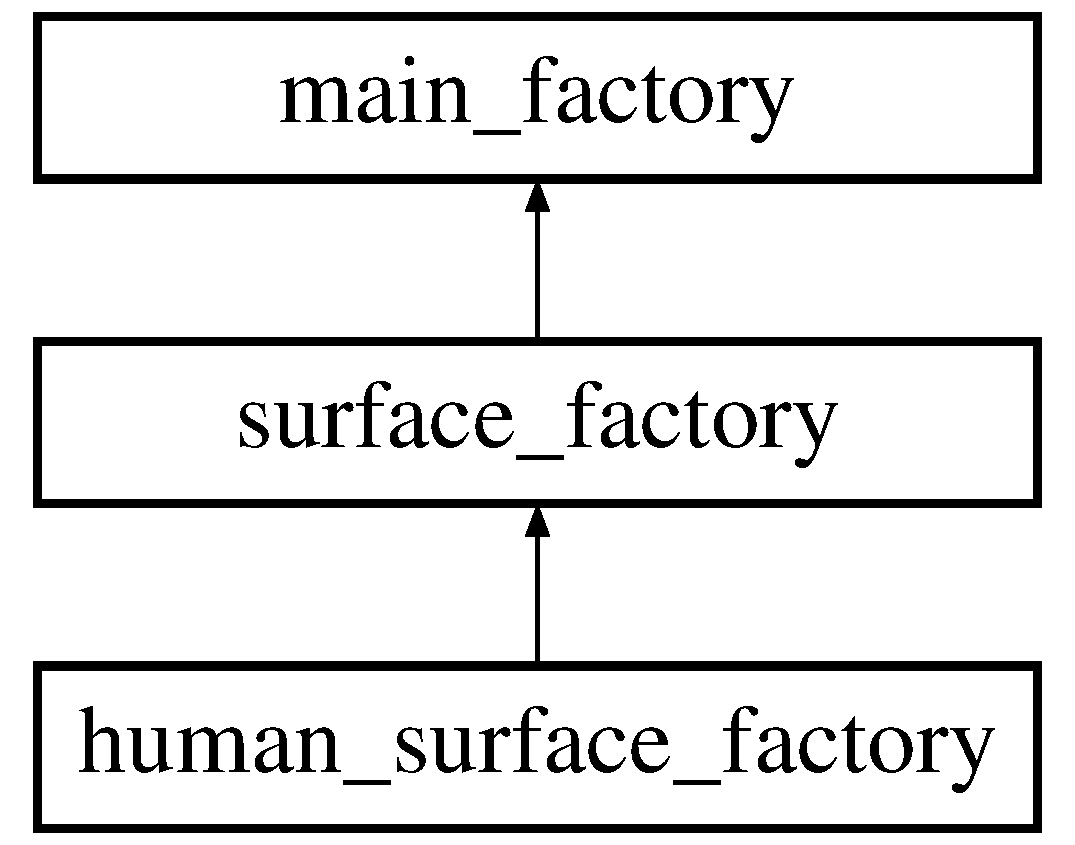
\includegraphics[height=3.000000cm]{classhuman__surface__factory}
\end{center}
\end{figure}
\subsection*{Public Member Functions}
\begin{DoxyCompactItemize}
\item 
\mbox{\Hypertarget{classhuman__surface__factory_a984dedfbbad2780353803058f58e6de6}\label{classhuman__surface__factory_a984dedfbbad2780353803058f58e6de6}} 
\mbox{\hyperlink{classsmall__mecha}{small\+\_\+mecha}} $\ast$ {\bfseries build\+\_\+fast\+\_\+unit} () override
\item 
\mbox{\Hypertarget{classhuman__surface__factory_a84df519f23b3e9dabd739563d0b4c3a4}\label{classhuman__surface__factory_a84df519f23b3e9dabd739563d0b4c3a4}} 
\mbox{\hyperlink{classarmored__mecha}{armored\+\_\+mecha}} $\ast$ {\bfseries build\+\_\+armor\+\_\+unit} () override
\item 
\mbox{\Hypertarget{classhuman__surface__factory_a391c38907f903d5b20d3fd05a88871da}\label{classhuman__surface__factory_a391c38907f903d5b20d3fd05a88871da}} 
\mbox{\hyperlink{classfast__scout}{fast\+\_\+scout}} $\ast$ {\bfseries build\+\_\+scout} () override
\item 
\mbox{\hyperlink{classhuman__engineer}{human\+\_\+engineer}} $\ast$ \mbox{\hyperlink{classhuman__surface__factory_a9ededd3065e7550d90fe7038daf96564}{build\+\_\+engineer}} () override
\item 
\mbox{\Hypertarget{classhuman__surface__factory_af0a9fe1cbc284f9ebc80eea70b303c56}\label{classhuman__surface__factory_af0a9fe1cbc284f9ebc80eea70b303c56}} 
void {\bfseries ME} () override
\end{DoxyCompactItemize}
\subsection*{Additional Inherited Members}


\subsection{Member Function Documentation}
\mbox{\Hypertarget{classhuman__surface__factory_a9ededd3065e7550d90fe7038daf96564}\label{classhuman__surface__factory_a9ededd3065e7550d90fe7038daf96564}} 
\index{human\+\_\+surface\+\_\+factory@{human\+\_\+surface\+\_\+factory}!build\+\_\+engineer@{build\+\_\+engineer}}
\index{build\+\_\+engineer@{build\+\_\+engineer}!human\+\_\+surface\+\_\+factory@{human\+\_\+surface\+\_\+factory}}
\subsubsection{\texorpdfstring{build\+\_\+engineer()}{build\_engineer()}}
{\footnotesize\ttfamily \mbox{\hyperlink{classhuman__engineer}{human\+\_\+engineer}}$\ast$ human\+\_\+surface\+\_\+factory\+::build\+\_\+engineer (\begin{DoxyParamCaption}{ }\end{DoxyParamCaption})\hspace{0.3cm}{\ttfamily [inline]}, {\ttfamily [override]}, {\ttfamily [virtual]}}

func to build an engineer \begin{DoxyReturn}{Returns}
new engineer 
\end{DoxyReturn}


Reimplemented from \mbox{\hyperlink{classmain__factory_ac970fe346638331722123f2bb240b590}{main\+\_\+factory}}.



The documentation for this class was generated from the following file\+:\begin{DoxyCompactItemize}
\item 
human\+\_\+tree.\+h\end{DoxyCompactItemize}

\hypertarget{classmain__factory}{}\section{main\+\_\+factory Class Reference}
\label{classmain__factory}\index{main\+\_\+factory@{main\+\_\+factory}}


{\ttfamily \#include $<$main\+\_\+lib.\+h$>$}

Inheritance diagram for main\+\_\+factory\+:\begin{figure}[H]
\begin{center}
\leavevmode
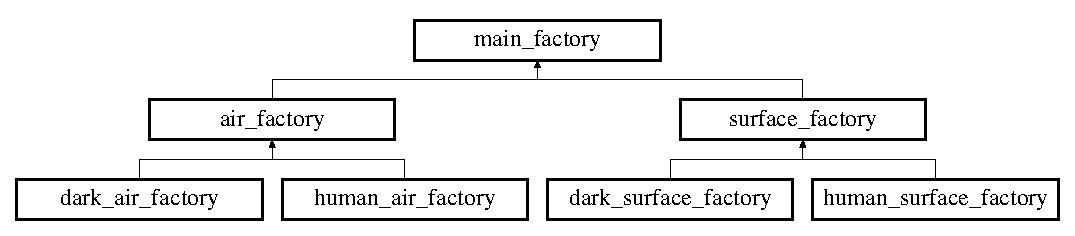
\includegraphics[height=2.727273cm]{classmain__factory}
\end{center}
\end{figure}
\subsection*{Public Member Functions}
\begin{DoxyCompactItemize}
\item 
virtual \mbox{\hyperlink{classunit__engineer}{unit\+\_\+engineer}} $\ast$ \mbox{\hyperlink{classmain__factory_ac970fe346638331722123f2bb240b590}{build\+\_\+engineer}} ()
\item 
const int \mbox{\hyperlink{classmain__factory_a91e3f57878aaa7b52d9ae4bcfbd84271}{get\+\_\+price}} ()
\end{DoxyCompactItemize}
\subsection*{Protected Member Functions}
\begin{DoxyCompactItemize}
\item 
\mbox{\Hypertarget{classmain__factory_ac392502ca0be0e5f42f714c4895a909e}\label{classmain__factory_ac392502ca0be0e5f42f714c4895a909e}} 
void {\bfseries set\+\_\+cost\+\_\+of\+\_\+factory} (int price)
\item 
\mbox{\Hypertarget{classmain__factory_a6f4ca8fd028cf672a67f7d4bba838cac}\label{classmain__factory_a6f4ca8fd028cf672a67f7d4bba838cac}} 
void {\bfseries set\+\_\+speed\+\_\+build} (int speed)
\end{DoxyCompactItemize}
\subsection*{Protected Attributes}
\begin{DoxyCompactItemize}
\item 
\mbox{\Hypertarget{classmain__factory_a76035fcad2dd7ee86e084b30240e6d8a}\label{classmain__factory_a76035fcad2dd7ee86e084b30240e6d8a}} 
int {\bfseries cost} = 0
\item 
\mbox{\Hypertarget{classmain__factory_aeffe2b762881074eef0c489d20e2aca3}\label{classmain__factory_aeffe2b762881074eef0c489d20e2aca3}} 
int {\bfseries speed\+\_\+of\+\_\+building\+\_\+units}
\end{DoxyCompactItemize}


\subsection{Detailed Description}
brief class for main factory 

\subsection{Member Function Documentation}
\mbox{\Hypertarget{classmain__factory_ac970fe346638331722123f2bb240b590}\label{classmain__factory_ac970fe346638331722123f2bb240b590}} 
\index{main\+\_\+factory@{main\+\_\+factory}!build\+\_\+engineer@{build\+\_\+engineer}}
\index{build\+\_\+engineer@{build\+\_\+engineer}!main\+\_\+factory@{main\+\_\+factory}}
\subsubsection{\texorpdfstring{build\+\_\+engineer()}{build\_engineer()}}
{\footnotesize\ttfamily virtual \mbox{\hyperlink{classunit__engineer}{unit\+\_\+engineer}}$\ast$ main\+\_\+factory\+::build\+\_\+engineer (\begin{DoxyParamCaption}{ }\end{DoxyParamCaption})\hspace{0.3cm}{\ttfamily [inline]}, {\ttfamily [virtual]}}

func to build an engineer \begin{DoxyReturn}{Returns}
new engineer 
\end{DoxyReturn}


Reimplemented in \mbox{\hyperlink{classhuman__air__factory_a34707f920a66afe9af4d5b0ecef8b2a7}{human\+\_\+air\+\_\+factory}}, \mbox{\hyperlink{classdark__air__factory_aaabd99e42553b5514b2fae2967bc3248}{dark\+\_\+air\+\_\+factory}}, \mbox{\hyperlink{classhuman__surface__factory_a9ededd3065e7550d90fe7038daf96564}{human\+\_\+surface\+\_\+factory}}, and \mbox{\hyperlink{classdark__surface__factory_a70172395b97a039eed8e3ff193f9f6a6}{dark\+\_\+surface\+\_\+factory}}.

\mbox{\Hypertarget{classmain__factory_a91e3f57878aaa7b52d9ae4bcfbd84271}\label{classmain__factory_a91e3f57878aaa7b52d9ae4bcfbd84271}} 
\index{main\+\_\+factory@{main\+\_\+factory}!get\+\_\+price@{get\+\_\+price}}
\index{get\+\_\+price@{get\+\_\+price}!main\+\_\+factory@{main\+\_\+factory}}
\subsubsection{\texorpdfstring{get\+\_\+price()}{get\_price()}}
{\footnotesize\ttfamily const int main\+\_\+factory\+::get\+\_\+price (\begin{DoxyParamCaption}{ }\end{DoxyParamCaption})\hspace{0.3cm}{\ttfamily [inline]}}

brief returns price of factory \begin{DoxyReturn}{Returns}

\end{DoxyReturn}


The documentation for this class was generated from the following file\+:\begin{DoxyCompactItemize}
\item 
main\+\_\+lib.\+h\end{DoxyCompactItemize}

\hypertarget{classmain__unit}{}\section{main\+\_\+unit Class Reference}
\label{classmain__unit}\index{main\+\_\+unit@{main\+\_\+unit}}


{\ttfamily \#include $<$main\+\_\+lib.\+h$>$}

Inheritance diagram for main\+\_\+unit\+:\begin{figure}[H]
\begin{center}
\leavevmode
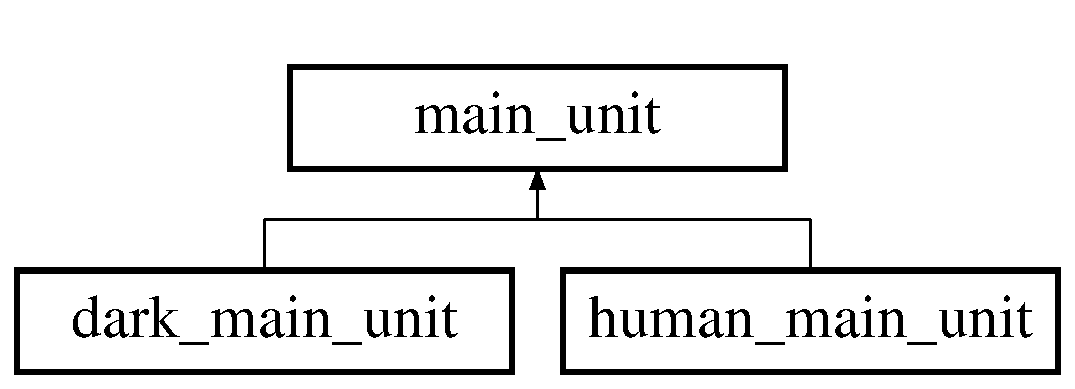
\includegraphics[height=2.000000cm]{classmain__unit}
\end{center}
\end{figure}
\subsection*{Public Member Functions}
\begin{DoxyCompactItemize}
\item 
\mbox{\Hypertarget{classmain__unit_a226de91180dca209eb398dda823f6f69}\label{classmain__unit_a226de91180dca209eb398dda823f6f69}} 
void {\bfseries create\+\_\+generator} ()
\item 
\mbox{\Hypertarget{classmain__unit_ab6994195071b8ffa812172a4b92a3d11}\label{classmain__unit_ab6994195071b8ffa812172a4b92a3d11}} 
virtual \mbox{\hyperlink{classsurface__factory}{surface\+\_\+factory}} $\ast$ {\bfseries create\+\_\+surface\+\_\+factory} ()
\item 
\mbox{\Hypertarget{classmain__unit_a0d7fc9e354ea63f687ba9d71c8933abb}\label{classmain__unit_a0d7fc9e354ea63f687ba9d71c8933abb}} 
virtual \mbox{\hyperlink{classair__factory}{air\+\_\+factory}} $\ast$ {\bfseries create\+\_\+air\+\_\+factory} ()
\item 
\mbox{\Hypertarget{classmain__unit_a167578355ad77cf9ae47dba2050c781e}\label{classmain__unit_a167578355ad77cf9ae47dba2050c781e}} 
virtual void {\bfseries who\+\_\+am\+\_\+i} ()
\end{DoxyCompactItemize}


\subsection{Detailed Description}
brief special main unit that commands everything 

The documentation for this class was generated from the following file\+:\begin{DoxyCompactItemize}
\item 
main\+\_\+lib.\+h\end{DoxyCompactItemize}

\hypertarget{classsmall__mecha}{}\section{small\+\_\+mecha Class Reference}
\label{classsmall__mecha}\index{small\+\_\+mecha@{small\+\_\+mecha}}
Inheritance diagram for small\+\_\+mecha\+:\begin{figure}[H]
\begin{center}
\leavevmode
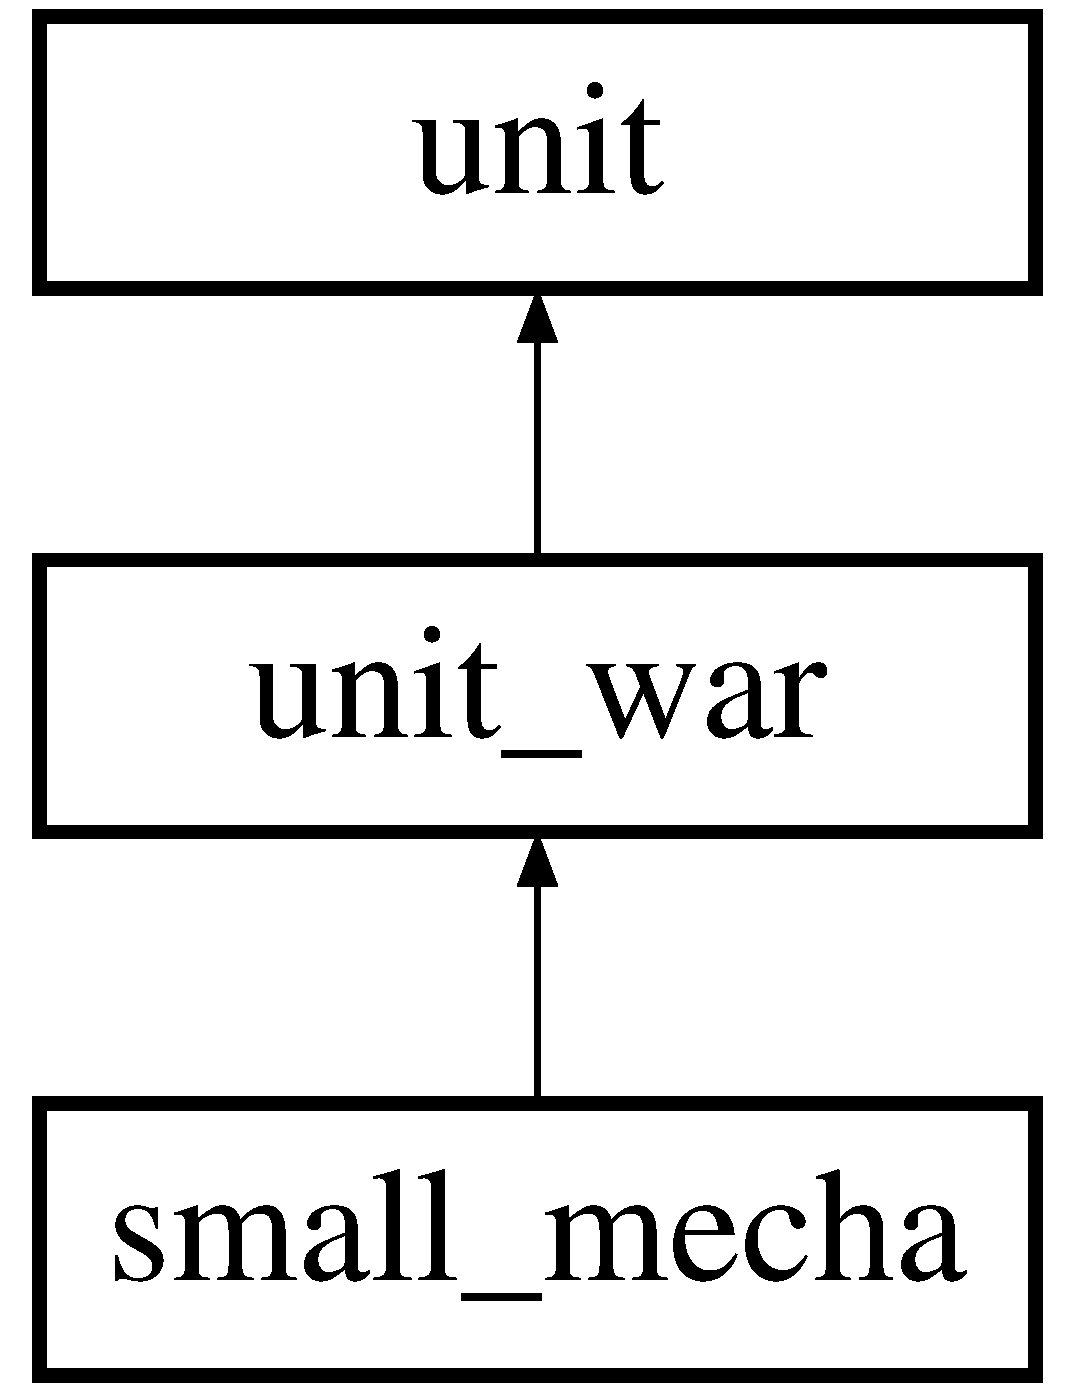
\includegraphics[height=3.000000cm]{classsmall__mecha}
\end{center}
\end{figure}
\subsection*{Public Member Functions}
\begin{DoxyCompactItemize}
\item 
\mbox{\Hypertarget{classsmall__mecha_abfaf595a7874e178ef9dc2e6cf300a13}\label{classsmall__mecha_abfaf595a7874e178ef9dc2e6cf300a13}} 
void {\bfseries get\+\_\+health} ()
\item 
\mbox{\Hypertarget{classsmall__mecha_a6ca1bc2683c75e4a095865d0123cdb20}\label{classsmall__mecha_a6ca1bc2683c75e4a095865d0123cdb20}} 
int {\bfseries get\+\_\+healthy} ()
\end{DoxyCompactItemize}
\subsection*{Additional Inherited Members}


The documentation for this class was generated from the following file\+:\begin{DoxyCompactItemize}
\item 
human\+\_\+tree.\+h\end{DoxyCompactItemize}

\hypertarget{classsquad}{}\section{squad Class Reference}
\label{classsquad}\index{squad@{squad}}


{\ttfamily \#include $<$squad.\+h$>$}

Inheritance diagram for squad\+:\begin{figure}[H]
\begin{center}
\leavevmode
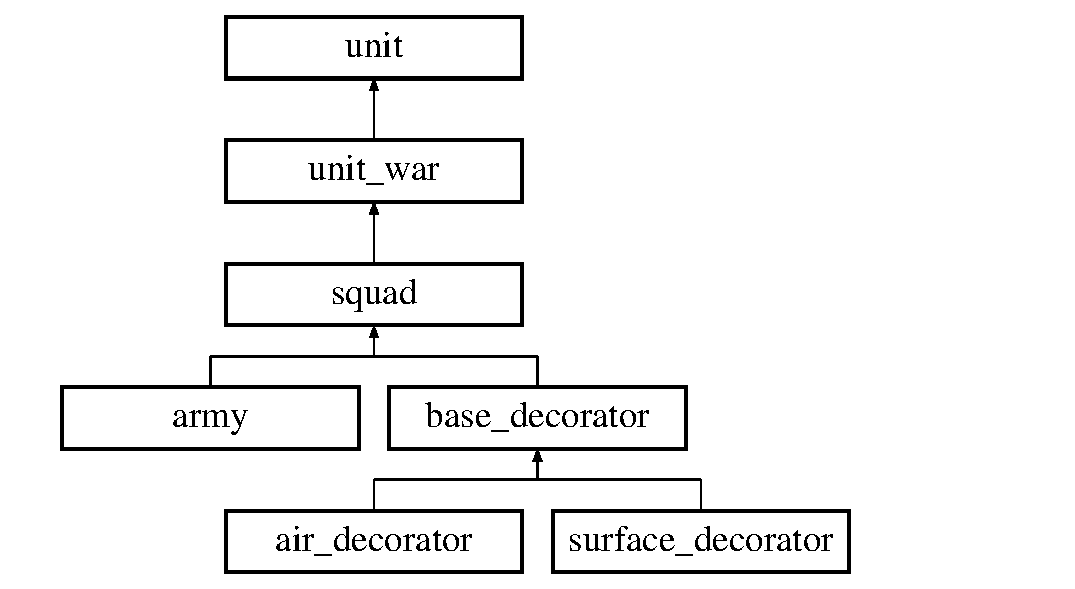
\includegraphics[height=5.000000cm]{classsquad}
\end{center}
\end{figure}
\subsection*{Public Member Functions}
\begin{DoxyCompactItemize}
\item 
const int \mbox{\hyperlink{classsquad_a7e719229279a2dd4948f1949d2fe2ccc}{get\+\_\+power}} () override
\item 
const int \mbox{\hyperlink{classsquad_a3b0a216e733b85a86721d4cef8c61f09}{get\+\_\+number}} () override
\item 
const int \mbox{\hyperlink{classsquad_a61378460e6a249acba2c201572449691}{get\+\_\+speed}} () override
\item 
\mbox{\Hypertarget{classsquad_ada3e4ba8d6b12a0cfbe26d7c5cf676a1}\label{classsquad_ada3e4ba8d6b12a0cfbe26d7c5cf676a1}} 
void {\bfseries add} (\mbox{\hyperlink{classunit__war}{unit\+\_\+war}} $\ast$reinforcement)
\item 
const int \mbox{\hyperlink{classsquad_ac3655293ec84ecdecd668b6bc0b76ec6}{get\+\_\+air\+\_\+deffence}} () override
\end{DoxyCompactItemize}
\subsection*{Public Attributes}
\begin{DoxyCompactItemize}
\item 
\mbox{\Hypertarget{classsquad_aa0258c60cdff4900cd897cabbd3de47f}\label{classsquad_aa0258c60cdff4900cd897cabbd3de47f}} 
std\+::vector$<$ \mbox{\hyperlink{classunit__war}{unit\+\_\+war}} $\ast$ $>$ {\bfseries units}
\end{DoxyCompactItemize}
\subsection*{Additional Inherited Members}


\subsection{Detailed Description}
brief a class which can contain some units one of the composite pattern part 

\subsection{Member Function Documentation}
\mbox{\Hypertarget{classsquad_ac3655293ec84ecdecd668b6bc0b76ec6}\label{classsquad_ac3655293ec84ecdecd668b6bc0b76ec6}} 
\index{squad@{squad}!get\+\_\+air\+\_\+deffence@{get\+\_\+air\+\_\+deffence}}
\index{get\+\_\+air\+\_\+deffence@{get\+\_\+air\+\_\+deffence}!squad@{squad}}
\subsubsection{\texorpdfstring{get\+\_\+air\+\_\+deffence()}{get\_air\_deffence()}}
{\footnotesize\ttfamily const int squad\+::get\+\_\+air\+\_\+deffence (\begin{DoxyParamCaption}{ }\end{DoxyParamCaption})\hspace{0.3cm}{\ttfamily [inline]}, {\ttfamily [override]}, {\ttfamily [virtual]}}

brief air\+\_\+defence power info \begin{DoxyReturn}{Returns}
air defence power 
\end{DoxyReturn}


Reimplemented from \mbox{\hyperlink{classunit__war_af26f2da420a828230a329339bc9ef805}{unit\+\_\+war}}.

\mbox{\Hypertarget{classsquad_a3b0a216e733b85a86721d4cef8c61f09}\label{classsquad_a3b0a216e733b85a86721d4cef8c61f09}} 
\index{squad@{squad}!get\+\_\+number@{get\+\_\+number}}
\index{get\+\_\+number@{get\+\_\+number}!squad@{squad}}
\subsubsection{\texorpdfstring{get\+\_\+number()}{get\_number()}}
{\footnotesize\ttfamily const int squad\+::get\+\_\+number (\begin{DoxyParamCaption}{ }\end{DoxyParamCaption})\hspace{0.3cm}{\ttfamily [inline]}, {\ttfamily [override]}, {\ttfamily [virtual]}}

brief just a func for composite pattern compatibility \begin{DoxyReturn}{Returns}
1 
\end{DoxyReturn}


Reimplemented from \mbox{\hyperlink{classunit_ab417b46197e2490f7fe279a9219e0f3c}{unit}}.

\mbox{\Hypertarget{classsquad_a7e719229279a2dd4948f1949d2fe2ccc}\label{classsquad_a7e719229279a2dd4948f1949d2fe2ccc}} 
\index{squad@{squad}!get\+\_\+power@{get\+\_\+power}}
\index{get\+\_\+power@{get\+\_\+power}!squad@{squad}}
\subsubsection{\texorpdfstring{get\+\_\+power()}{get\_power()}}
{\footnotesize\ttfamily const int squad\+::get\+\_\+power (\begin{DoxyParamCaption}{ }\end{DoxyParamCaption})\hspace{0.3cm}{\ttfamily [inline]}, {\ttfamily [override]}, {\ttfamily [virtual]}}

brief returns power of unit \begin{DoxyReturn}{Returns}
power of unit 
\end{DoxyReturn}


Reimplemented from \mbox{\hyperlink{classunit__war_adea1fced490739cf8b7a6e49ec90cf59}{unit\+\_\+war}}.

\mbox{\Hypertarget{classsquad_a61378460e6a249acba2c201572449691}\label{classsquad_a61378460e6a249acba2c201572449691}} 
\index{squad@{squad}!get\+\_\+speed@{get\+\_\+speed}}
\index{get\+\_\+speed@{get\+\_\+speed}!squad@{squad}}
\subsubsection{\texorpdfstring{get\+\_\+speed()}{get\_speed()}}
{\footnotesize\ttfamily const int squad\+::get\+\_\+speed (\begin{DoxyParamCaption}{ }\end{DoxyParamCaption})\hspace{0.3cm}{\ttfamily [inline]}, {\ttfamily [override]}, {\ttfamily [virtual]}}

brief returns max speed of unit \begin{DoxyReturn}{Returns}
max speed of unit 
\end{DoxyReturn}


Reimplemented from \mbox{\hyperlink{classunit_af81d18961574843ddaa5273bfb57cf7f}{unit}}.



The documentation for this class was generated from the following file\+:\begin{DoxyCompactItemize}
\item 
squad.\+h\end{DoxyCompactItemize}

\hypertarget{classsurface__decorator}{}\section{surface\+\_\+decorator Class Reference}
\label{classsurface__decorator}\index{surface\+\_\+decorator@{surface\+\_\+decorator}}


{\ttfamily \#include $<$surface\+\_\+decorator.\+h$>$}

Inheritance diagram for surface\+\_\+decorator\+:\begin{figure}[H]
\begin{center}
\leavevmode
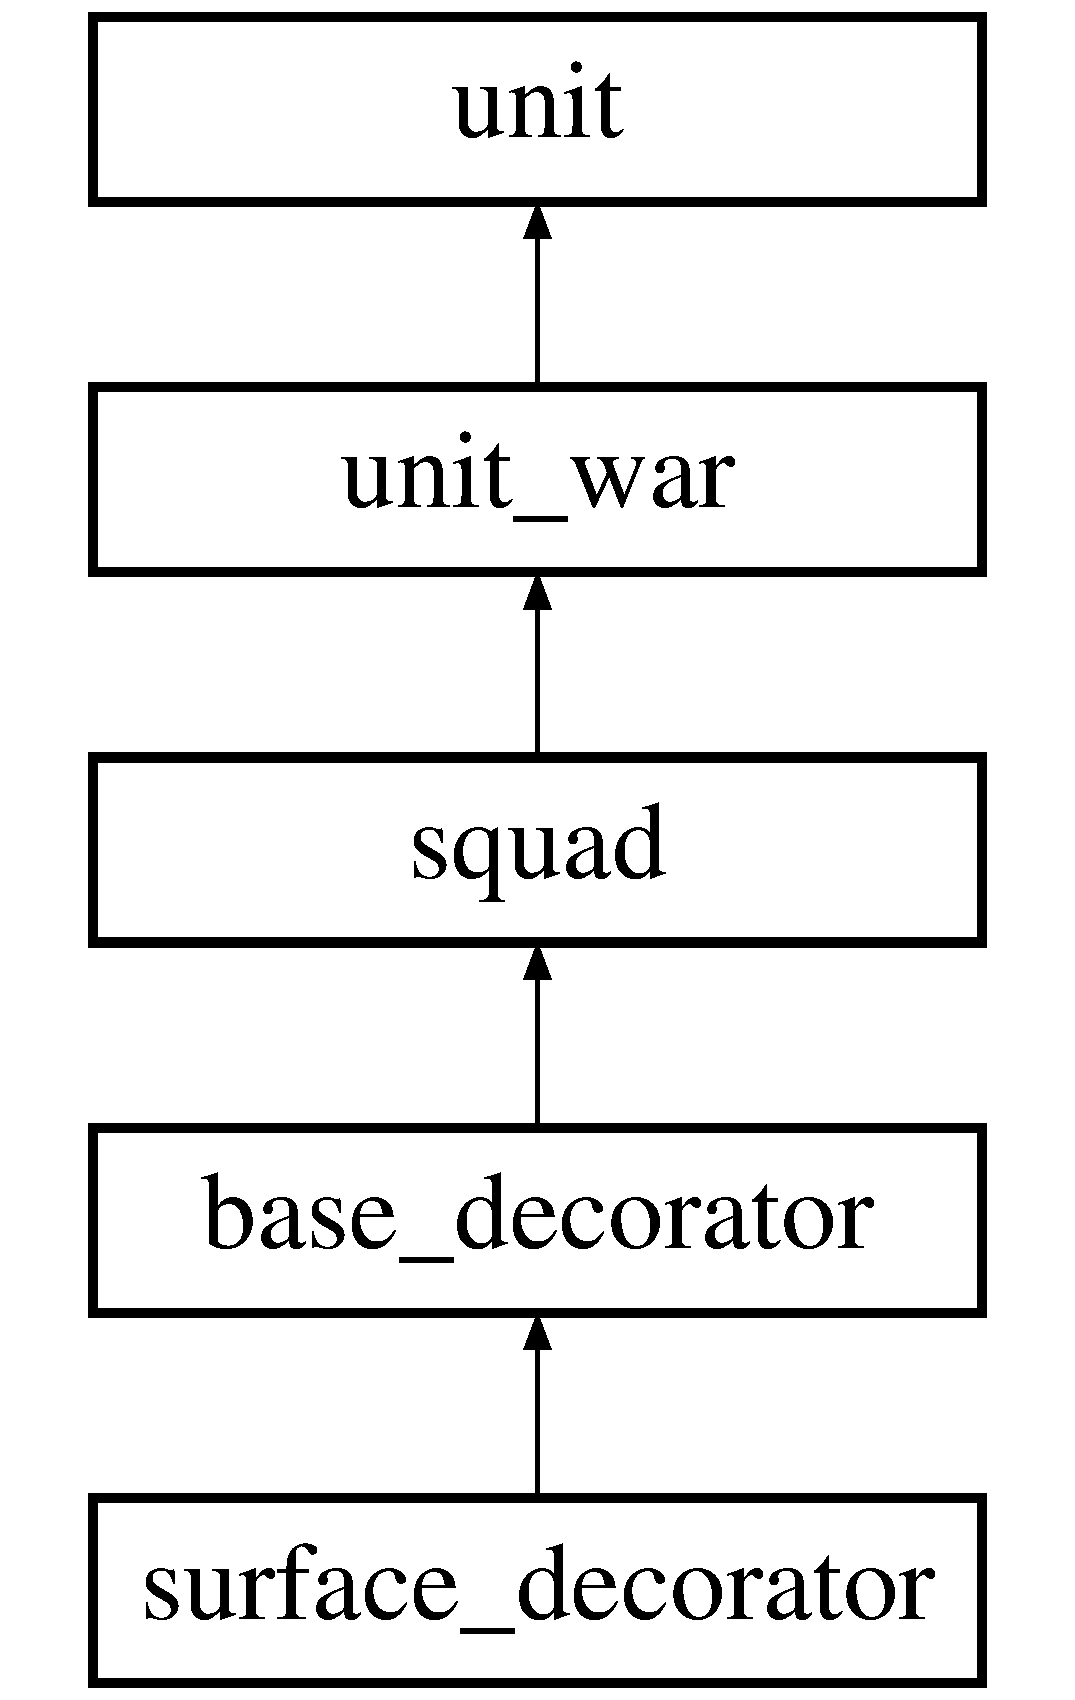
\includegraphics[height=5.000000cm]{classsurface__decorator}
\end{center}
\end{figure}
\subsection*{Additional Inherited Members}


\subsection{Detailed Description}
brief if army/squad will have to fight on surface it will be wrapped in this decorator 

The documentation for this class was generated from the following file\+:\begin{DoxyCompactItemize}
\item 
surface\+\_\+decorator.\+h\end{DoxyCompactItemize}

\hypertarget{classsurface__factory}{}\section{surface\+\_\+factory Class Reference}
\label{classsurface__factory}\index{surface\+\_\+factory@{surface\+\_\+factory}}


{\ttfamily \#include $<$main\+\_\+lib.\+h$>$}

Inheritance diagram for surface\+\_\+factory\+:\begin{figure}[H]
\begin{center}
\leavevmode
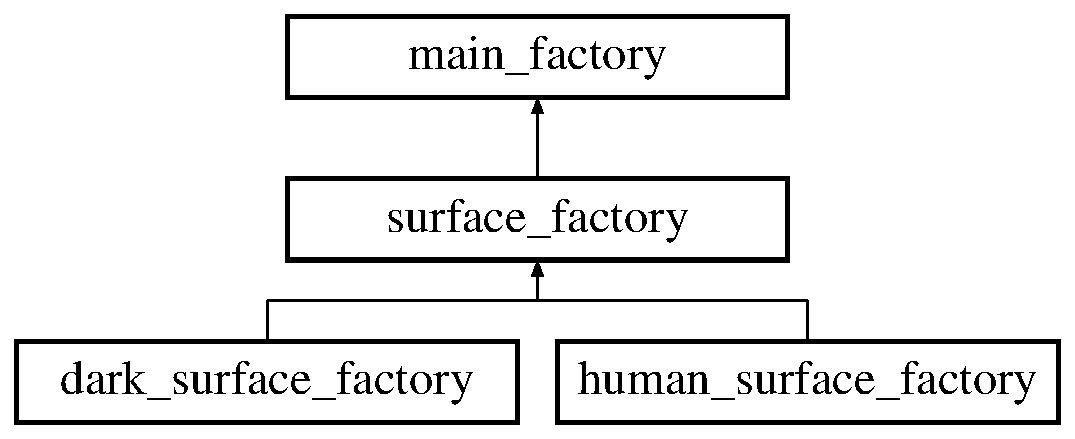
\includegraphics[height=3.000000cm]{classsurface__factory}
\end{center}
\end{figure}
\subsection*{Public Member Functions}
\begin{DoxyCompactItemize}
\item 
\mbox{\Hypertarget{classsurface__factory_a67054d75afd077764781cd101529f40c}\label{classsurface__factory_a67054d75afd077764781cd101529f40c}} 
virtual \mbox{\hyperlink{classunit__war}{unit\+\_\+war}} $\ast$ {\bfseries build\+\_\+airdefence} ()
\item 
\mbox{\Hypertarget{classsurface__factory_a0ad51809e3b62f821a7e35858f2ebe64}\label{classsurface__factory_a0ad51809e3b62f821a7e35858f2ebe64}} 
virtual \mbox{\hyperlink{classunit__war}{unit\+\_\+war}} $\ast$ {\bfseries build\+\_\+armor\+\_\+unit} ()
\item 
\mbox{\Hypertarget{classsurface__factory_aadb3805043973d0f157e0d7198503cb6}\label{classsurface__factory_aadb3805043973d0f157e0d7198503cb6}} 
virtual \mbox{\hyperlink{classunit__war}{unit\+\_\+war}} $\ast$ {\bfseries build\+\_\+fast\+\_\+unit} ()
\item 
\mbox{\Hypertarget{classsurface__factory_adeae2cd0024dd9422805623be9dfed39}\label{classsurface__factory_adeae2cd0024dd9422805623be9dfed39}} 
virtual \mbox{\hyperlink{classunit__war}{unit\+\_\+war}} $\ast$ {\bfseries build\+\_\+scout} ()
\item 
virtual \mbox{\hyperlink{classextra__unit__builder}{extra\+\_\+unit\+\_\+builder}} $\ast$ \mbox{\hyperlink{classsurface__factory_a7a75bc9c3cd6b38bfbdcd062498beffc}{build\+\_\+extra\+\_\+unit}} ()
\item 
\mbox{\Hypertarget{classsurface__factory_ac6555c8d0ec21ea580c988a4739d0f96}\label{classsurface__factory_ac6555c8d0ec21ea580c988a4739d0f96}} 
virtual void {\bfseries ME} ()
\end{DoxyCompactItemize}
\subsection*{Additional Inherited Members}


\subsection{Detailed Description}
special factory for surface 

\subsection{Member Function Documentation}
\mbox{\Hypertarget{classsurface__factory_a7a75bc9c3cd6b38bfbdcd062498beffc}\label{classsurface__factory_a7a75bc9c3cd6b38bfbdcd062498beffc}} 
\index{surface\+\_\+factory@{surface\+\_\+factory}!build\+\_\+extra\+\_\+unit@{build\+\_\+extra\+\_\+unit}}
\index{build\+\_\+extra\+\_\+unit@{build\+\_\+extra\+\_\+unit}!surface\+\_\+factory@{surface\+\_\+factory}}
\subsubsection{\texorpdfstring{build\+\_\+extra\+\_\+unit()}{build\_extra\_unit()}}
{\footnotesize\ttfamily virtual \mbox{\hyperlink{classextra__unit__builder}{extra\+\_\+unit\+\_\+builder}}$\ast$ surface\+\_\+factory\+::build\+\_\+extra\+\_\+unit (\begin{DoxyParamCaption}{ }\end{DoxyParamCaption})\hspace{0.3cm}{\ttfamily [inline]}, {\ttfamily [virtual]}}

func that builds extra unit \begin{DoxyReturn}{Returns}
new extra unit 
\end{DoxyReturn}


The documentation for this class was generated from the following file\+:\begin{DoxyCompactItemize}
\item 
main\+\_\+lib.\+h\end{DoxyCompactItemize}

\hypertarget{classunit}{}\section{unit Class Reference}
\label{classunit}\index{unit@{unit}}


{\ttfamily \#include $<$main\+\_\+lib.\+h$>$}

Inheritance diagram for unit\+:\begin{figure}[H]
\begin{center}
\leavevmode
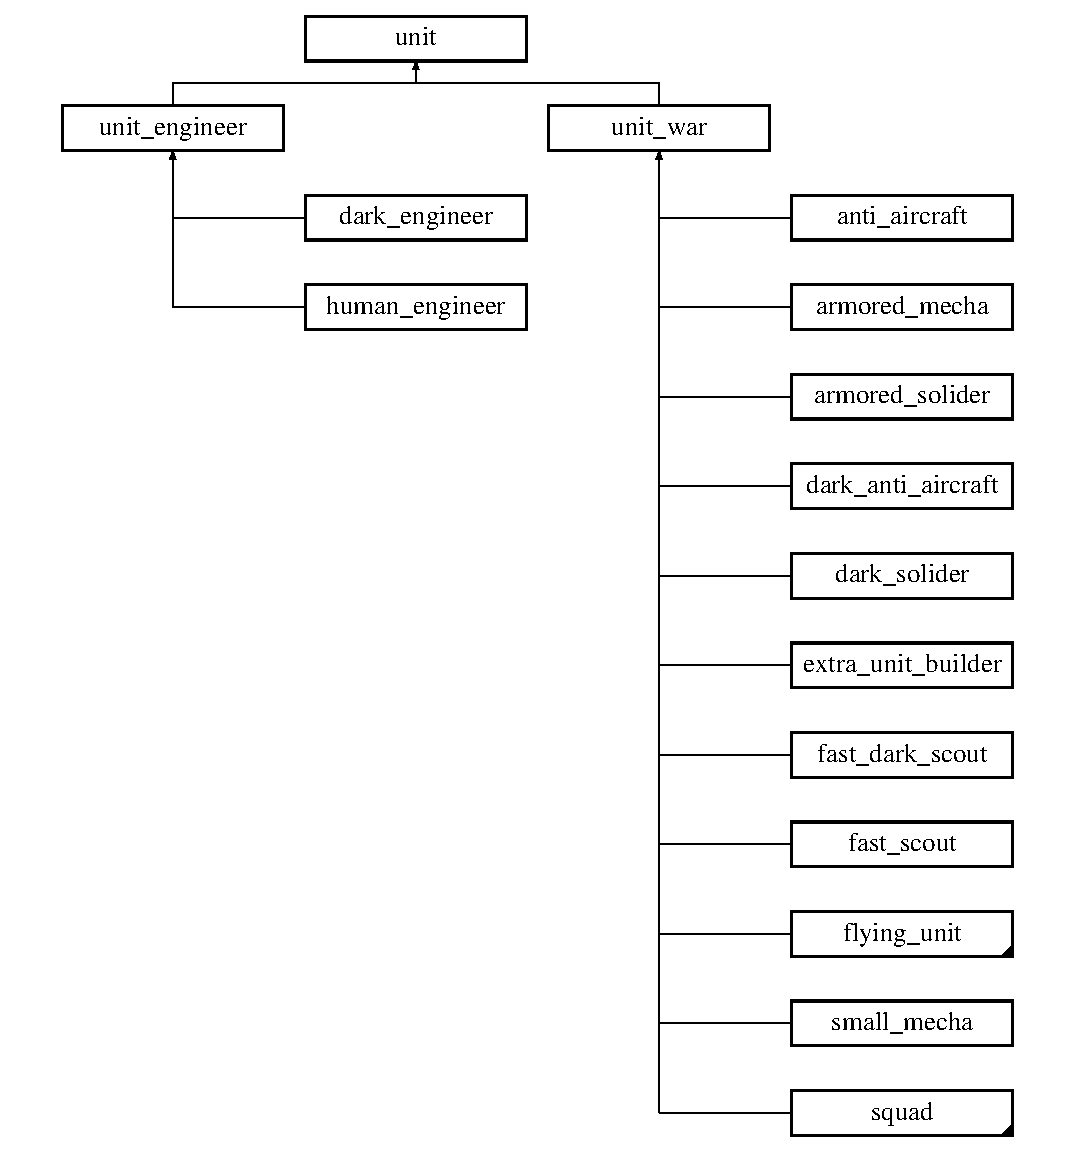
\includegraphics[height=12.000000cm]{classunit}
\end{center}
\end{figure}
\subsection*{Public Member Functions}
\begin{DoxyCompactItemize}
\item 
virtual const int \mbox{\hyperlink{classunit_a817ef860467c21c378deb39f738c33e0}{get\+\_\+cost}} ()
\item 
virtual const int \mbox{\hyperlink{classunit_af81d18961574843ddaa5273bfb57cf7f}{get\+\_\+speed}} ()
\item 
virtual const int \mbox{\hyperlink{classunit_ab417b46197e2490f7fe279a9219e0f3c}{get\+\_\+number}} ()
\end{DoxyCompactItemize}
\subsection*{Static Public Attributes}
\begin{DoxyCompactItemize}
\item 
\mbox{\Hypertarget{classunit_a31777e05331f1b9253a487820eaf5e3c}\label{classunit_a31777e05331f1b9253a487820eaf5e3c}} 
static int {\bfseries amount\+\_\+of\+\_\+units} = 0
\end{DoxyCompactItemize}
\subsection*{Protected Member Functions}
\begin{DoxyCompactItemize}
\item 
virtual void \mbox{\hyperlink{classunit_a3b2dbfe9c1daaf2b8ef6b604d7803dc2}{set\+\_\+speed}} (int a)
\item 
virtual void \mbox{\hyperlink{classunit_a1dabc406074919750b1c606496e8e42d}{set\+\_\+health}} (int c)
\item 
void \mbox{\hyperlink{classunit_a1f7b84a24ff09c2653e5c6d2d046472e}{set\+\_\+cost}} (int price)
\end{DoxyCompactItemize}
\subsection*{Protected Attributes}
\begin{DoxyCompactItemize}
\item 
\mbox{\Hypertarget{classunit_aeefab70a4b68985ea17e1acf9694e765}\label{classunit_aeefab70a4b68985ea17e1acf9694e765}} 
int {\bfseries health}
\item 
\mbox{\Hypertarget{classunit_aa5cd467b54f26a2bf446ba27d913d035}\label{classunit_aa5cd467b54f26a2bf446ba27d913d035}} 
int {\bfseries speed}
\item 
\mbox{\Hypertarget{classunit_a9101170be3651fe1f7169ab7275715b1}\label{classunit_a9101170be3651fe1f7169ab7275715b1}} 
int {\bfseries energy\+\_\+cost}
\end{DoxyCompactItemize}


\subsection{Detailed Description}
brief main class for unit in this game 

\subsection{Member Function Documentation}
\mbox{\Hypertarget{classunit_a817ef860467c21c378deb39f738c33e0}\label{classunit_a817ef860467c21c378deb39f738c33e0}} 
\index{unit@{unit}!get\+\_\+cost@{get\+\_\+cost}}
\index{get\+\_\+cost@{get\+\_\+cost}!unit@{unit}}
\subsubsection{\texorpdfstring{get\+\_\+cost()}{get\_cost()}}
{\footnotesize\ttfamily virtual const int unit\+::get\+\_\+cost (\begin{DoxyParamCaption}{ }\end{DoxyParamCaption})\hspace{0.3cm}{\ttfamily [inline]}, {\ttfamily [virtual]}}

func that returns cost of the unit \begin{DoxyReturn}{Returns}
cost of the unit 
\end{DoxyReturn}


Reimplemented in \mbox{\hyperlink{classextra__unit__builder_a84ce334361c5acd1a59775a74fabde86}{extra\+\_\+unit\+\_\+builder}}.

\mbox{\Hypertarget{classunit_ab417b46197e2490f7fe279a9219e0f3c}\label{classunit_ab417b46197e2490f7fe279a9219e0f3c}} 
\index{unit@{unit}!get\+\_\+number@{get\+\_\+number}}
\index{get\+\_\+number@{get\+\_\+number}!unit@{unit}}
\subsubsection{\texorpdfstring{get\+\_\+number()}{get\_number()}}
{\footnotesize\ttfamily virtual const int unit\+::get\+\_\+number (\begin{DoxyParamCaption}{ }\end{DoxyParamCaption})\hspace{0.3cm}{\ttfamily [inline]}, {\ttfamily [virtual]}}

brief just a func for composite pattern compatibility \begin{DoxyReturn}{Returns}
1 
\end{DoxyReturn}


Reimplemented in \mbox{\hyperlink{classsquad_a3b0a216e733b85a86721d4cef8c61f09}{squad}}.

\mbox{\Hypertarget{classunit_af81d18961574843ddaa5273bfb57cf7f}\label{classunit_af81d18961574843ddaa5273bfb57cf7f}} 
\index{unit@{unit}!get\+\_\+speed@{get\+\_\+speed}}
\index{get\+\_\+speed@{get\+\_\+speed}!unit@{unit}}
\subsubsection{\texorpdfstring{get\+\_\+speed()}{get\_speed()}}
{\footnotesize\ttfamily virtual const int unit\+::get\+\_\+speed (\begin{DoxyParamCaption}{ }\end{DoxyParamCaption})\hspace{0.3cm}{\ttfamily [inline]}, {\ttfamily [virtual]}}

brief returns max speed of unit \begin{DoxyReturn}{Returns}
max speed of unit 
\end{DoxyReturn}


Reimplemented in \mbox{\hyperlink{classsquad_a61378460e6a249acba2c201572449691}{squad}}.

\mbox{\Hypertarget{classunit_a1f7b84a24ff09c2653e5c6d2d046472e}\label{classunit_a1f7b84a24ff09c2653e5c6d2d046472e}} 
\index{unit@{unit}!set\+\_\+cost@{set\+\_\+cost}}
\index{set\+\_\+cost@{set\+\_\+cost}!unit@{unit}}
\subsubsection{\texorpdfstring{set\+\_\+cost()}{set\_cost()}}
{\footnotesize\ttfamily void unit\+::set\+\_\+cost (\begin{DoxyParamCaption}\item[{int}]{price }\end{DoxyParamCaption})\hspace{0.3cm}{\ttfamily [inline]}, {\ttfamily [protected]}}

brief sets cost of the unit 
\begin{DoxyParams}{Parameters}
{\em price} & \\
\hline
\end{DoxyParams}
\mbox{\Hypertarget{classunit_a1dabc406074919750b1c606496e8e42d}\label{classunit_a1dabc406074919750b1c606496e8e42d}} 
\index{unit@{unit}!set\+\_\+health@{set\+\_\+health}}
\index{set\+\_\+health@{set\+\_\+health}!unit@{unit}}
\subsubsection{\texorpdfstring{set\+\_\+health()}{set\_health()}}
{\footnotesize\ttfamily virtual void unit\+::set\+\_\+health (\begin{DoxyParamCaption}\item[{int}]{c }\end{DoxyParamCaption})\hspace{0.3cm}{\ttfamily [inline]}, {\ttfamily [protected]}, {\ttfamily [virtual]}}

brief sets health of unit 
\begin{DoxyParams}{Parameters}
{\em c} & \\
\hline
\end{DoxyParams}


Reimplemented in \mbox{\hyperlink{classextra__unit__builder_a7471f05c65d3f2c230c405ec0bcdaa7d}{extra\+\_\+unit\+\_\+builder}}.

\mbox{\Hypertarget{classunit_a3b2dbfe9c1daaf2b8ef6b604d7803dc2}\label{classunit_a3b2dbfe9c1daaf2b8ef6b604d7803dc2}} 
\index{unit@{unit}!set\+\_\+speed@{set\+\_\+speed}}
\index{set\+\_\+speed@{set\+\_\+speed}!unit@{unit}}
\subsubsection{\texorpdfstring{set\+\_\+speed()}{set\_speed()}}
{\footnotesize\ttfamily virtual void unit\+::set\+\_\+speed (\begin{DoxyParamCaption}\item[{int}]{a }\end{DoxyParamCaption})\hspace{0.3cm}{\ttfamily [inline]}, {\ttfamily [protected]}, {\ttfamily [virtual]}}

brief sets speed of unit 
\begin{DoxyParams}{Parameters}
{\em a} & \\
\hline
\end{DoxyParams}


Reimplemented in \mbox{\hyperlink{classextra__unit__builder_aa95d6dcfba85a06592d6725baebd51cc}{extra\+\_\+unit\+\_\+builder}}.



The documentation for this class was generated from the following file\+:\begin{DoxyCompactItemize}
\item 
main\+\_\+lib.\+h\end{DoxyCompactItemize}

\hypertarget{classunit__engineer}{}\section{unit\+\_\+engineer Class Reference}
\label{classunit__engineer}\index{unit\+\_\+engineer@{unit\+\_\+engineer}}


{\ttfamily \#include $<$main\+\_\+lib.\+h$>$}

Inheritance diagram for unit\+\_\+engineer\+:\begin{figure}[H]
\begin{center}
\leavevmode
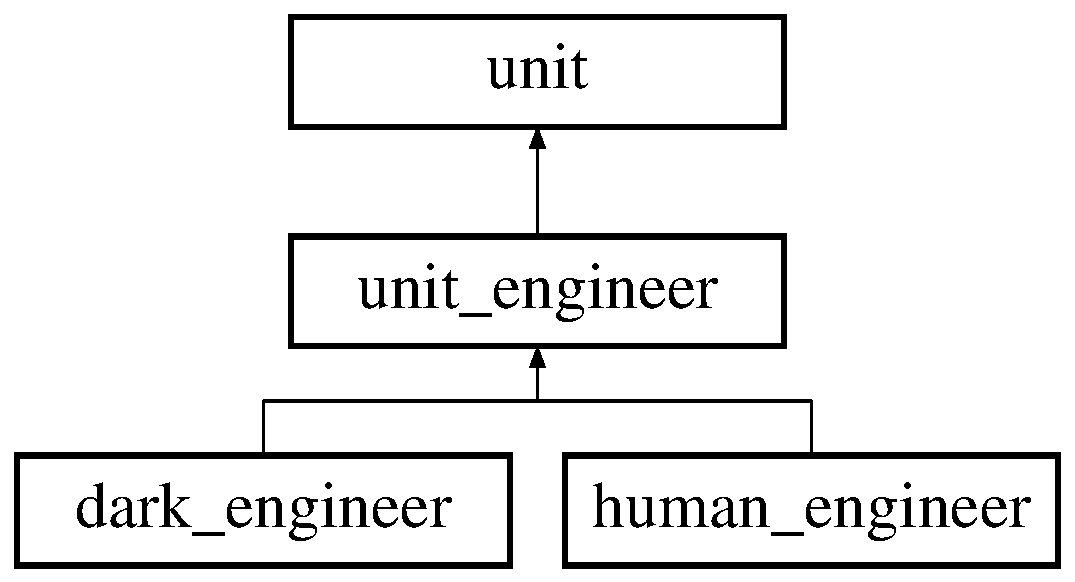
\includegraphics[height=3.000000cm]{classunit__engineer}
\end{center}
\end{figure}
\subsection*{Public Member Functions}
\begin{DoxyCompactItemize}
\item 
const int \mbox{\hyperlink{classunit__engineer_a9f3149789f1883a468132a20a96bc7b7}{get\+\_\+speed\+\_\+of\+\_\+engineer}} ()
\end{DoxyCompactItemize}
\subsection*{Protected Member Functions}
\begin{DoxyCompactItemize}
\item 
void \mbox{\hyperlink{classunit__engineer_a76ac2640e3e83af2d07c99d124331c12}{set\+\_\+speed\+\_\+of\+\_\+building}} (int setted\+\_\+speed)
\end{DoxyCompactItemize}
\subsection*{Additional Inherited Members}


\subsection{Detailed Description}
brief unit that can build something 

\subsection{Member Function Documentation}
\mbox{\Hypertarget{classunit__engineer_a9f3149789f1883a468132a20a96bc7b7}\label{classunit__engineer_a9f3149789f1883a468132a20a96bc7b7}} 
\index{unit\+\_\+engineer@{unit\+\_\+engineer}!get\+\_\+speed\+\_\+of\+\_\+engineer@{get\+\_\+speed\+\_\+of\+\_\+engineer}}
\index{get\+\_\+speed\+\_\+of\+\_\+engineer@{get\+\_\+speed\+\_\+of\+\_\+engineer}!unit\+\_\+engineer@{unit\+\_\+engineer}}
\subsubsection{\texorpdfstring{get\+\_\+speed\+\_\+of\+\_\+engineer()}{get\_speed\_of\_engineer()}}
{\footnotesize\ttfamily const int unit\+\_\+engineer\+::get\+\_\+speed\+\_\+of\+\_\+engineer (\begin{DoxyParamCaption}{ }\end{DoxyParamCaption})\hspace{0.3cm}{\ttfamily [inline]}}

brief gets speed of engineers \begin{DoxyReturn}{Returns}
speed of building of engineers 
\end{DoxyReturn}
\mbox{\Hypertarget{classunit__engineer_a76ac2640e3e83af2d07c99d124331c12}\label{classunit__engineer_a76ac2640e3e83af2d07c99d124331c12}} 
\index{unit\+\_\+engineer@{unit\+\_\+engineer}!set\+\_\+speed\+\_\+of\+\_\+building@{set\+\_\+speed\+\_\+of\+\_\+building}}
\index{set\+\_\+speed\+\_\+of\+\_\+building@{set\+\_\+speed\+\_\+of\+\_\+building}!unit\+\_\+engineer@{unit\+\_\+engineer}}
\subsubsection{\texorpdfstring{set\+\_\+speed\+\_\+of\+\_\+building()}{set\_speed\_of\_building()}}
{\footnotesize\ttfamily void unit\+\_\+engineer\+::set\+\_\+speed\+\_\+of\+\_\+building (\begin{DoxyParamCaption}\item[{int}]{setted\+\_\+speed }\end{DoxyParamCaption})\hspace{0.3cm}{\ttfamily [inline]}, {\ttfamily [protected]}}

brief sets speed which will use engineer to build something 
\begin{DoxyParams}{Parameters}
{\em setted\+\_\+speed} & \\
\hline
\end{DoxyParams}


The documentation for this class was generated from the following file\+:\begin{DoxyCompactItemize}
\item 
main\+\_\+lib.\+h\end{DoxyCompactItemize}

\hypertarget{classunit__main}{}\section{unit\+\_\+main Class Reference}
\label{classunit__main}\index{unit\+\_\+main@{unit\+\_\+main}}


The documentation for this class was generated from the following file\+:\begin{DoxyCompactItemize}
\item 
main\+\_\+lib.\+h\end{DoxyCompactItemize}

\hypertarget{classunit__war}{}\section{unit\+\_\+war Class Reference}
\label{classunit__war}\index{unit\+\_\+war@{unit\+\_\+war}}


{\ttfamily \#include $<$main\+\_\+lib.\+h$>$}

Inheritance diagram for unit\+\_\+war\+:\begin{figure}[H]
\begin{center}
\leavevmode
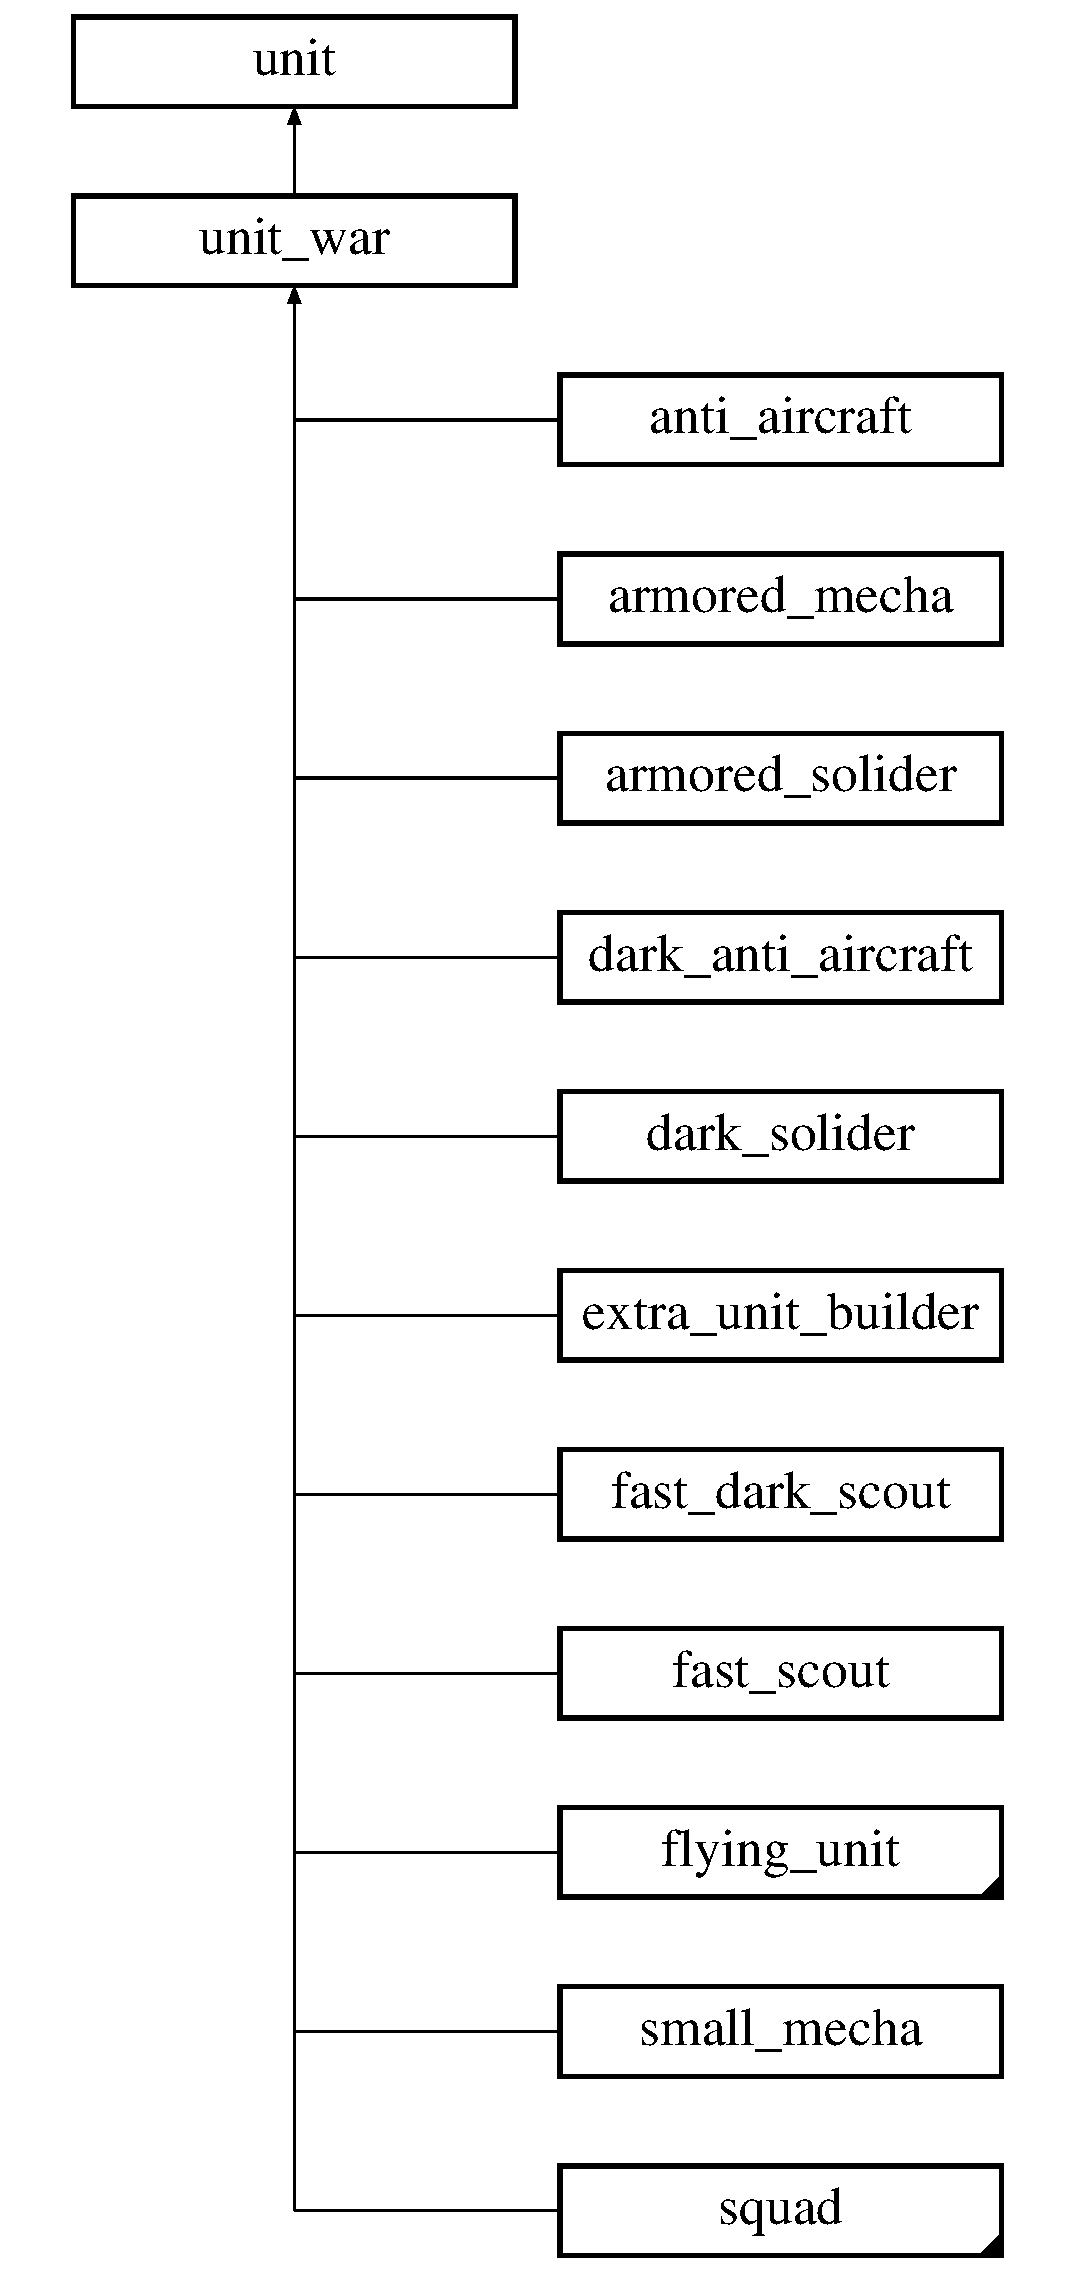
\includegraphics[height=12.000000cm]{classunit__war}
\end{center}
\end{figure}
\subsection*{Public Member Functions}
\begin{DoxyCompactItemize}
\item 
virtual const int \mbox{\hyperlink{classunit__war_adea1fced490739cf8b7a6e49ec90cf59}{get\+\_\+power}} ()
\item 
virtual const int \mbox{\hyperlink{classunit__war_af26f2da420a828230a329339bc9ef805}{get\+\_\+air\+\_\+deffence}} ()
\end{DoxyCompactItemize}
\subsection*{Protected Member Functions}
\begin{DoxyCompactItemize}
\item 
virtual void \mbox{\hyperlink{classunit__war_a8ea09eb3e352d5a3b2d7611ac78124a2}{set\+\_\+power}} (int b)
\item 
void \mbox{\hyperlink{classunit__war_ae171887cd752f92cee8cc4e32c541684}{decrease\+\_\+health}} (int damage)
\item 
void \mbox{\hyperlink{classunit__war_a9f1ae061c0761d35bdaaac8098d69dd0}{attack}} ()
\end{DoxyCompactItemize}
\subsection*{Protected Attributes}
\begin{DoxyCompactItemize}
\item 
\mbox{\Hypertarget{classunit__war_a05e852a78db3b69cbbf0b73a568f9dc2}\label{classunit__war_a05e852a78db3b69cbbf0b73a568f9dc2}} 
int {\bfseries power}
\end{DoxyCompactItemize}
\subsection*{Additional Inherited Members}


\subsection{Detailed Description}
brief main prototype for units created for battles 

\subsection{Member Function Documentation}
\mbox{\Hypertarget{classunit__war_a9f1ae061c0761d35bdaaac8098d69dd0}\label{classunit__war_a9f1ae061c0761d35bdaaac8098d69dd0}} 
\index{unit\+\_\+war@{unit\+\_\+war}!attack@{attack}}
\index{attack@{attack}!unit\+\_\+war@{unit\+\_\+war}}
\subsubsection{\texorpdfstring{attack()}{attack()}}
{\footnotesize\ttfamily void unit\+\_\+war\+::attack (\begin{DoxyParamCaption}{ }\end{DoxyParamCaption})\hspace{0.3cm}{\ttfamily [inline]}, {\ttfamily [protected]}}

brief attacks someone \mbox{\Hypertarget{classunit__war_ae171887cd752f92cee8cc4e32c541684}\label{classunit__war_ae171887cd752f92cee8cc4e32c541684}} 
\index{unit\+\_\+war@{unit\+\_\+war}!decrease\+\_\+health@{decrease\+\_\+health}}
\index{decrease\+\_\+health@{decrease\+\_\+health}!unit\+\_\+war@{unit\+\_\+war}}
\subsubsection{\texorpdfstring{decrease\+\_\+health()}{decrease\_health()}}
{\footnotesize\ttfamily void unit\+\_\+war\+::decrease\+\_\+health (\begin{DoxyParamCaption}\item[{int}]{damage }\end{DoxyParamCaption})\hspace{0.3cm}{\ttfamily [inline]}, {\ttfamily [protected]}}

brief decreases health during battle 
\begin{DoxyParams}{Parameters}
{\em damage} & \\
\hline
\end{DoxyParams}
\mbox{\Hypertarget{classunit__war_af26f2da420a828230a329339bc9ef805}\label{classunit__war_af26f2da420a828230a329339bc9ef805}} 
\index{unit\+\_\+war@{unit\+\_\+war}!get\+\_\+air\+\_\+deffence@{get\+\_\+air\+\_\+deffence}}
\index{get\+\_\+air\+\_\+deffence@{get\+\_\+air\+\_\+deffence}!unit\+\_\+war@{unit\+\_\+war}}
\subsubsection{\texorpdfstring{get\+\_\+air\+\_\+deffence()}{get\_air\_deffence()}}
{\footnotesize\ttfamily virtual const int unit\+\_\+war\+::get\+\_\+air\+\_\+deffence (\begin{DoxyParamCaption}{ }\end{DoxyParamCaption})\hspace{0.3cm}{\ttfamily [inline]}, {\ttfamily [virtual]}}

brief air\+\_\+defence power info \begin{DoxyReturn}{Returns}
air defence power 
\end{DoxyReturn}


Reimplemented in \mbox{\hyperlink{classflying__unit_a47dbbf3832a5b5e8f5365d87cdbfddab}{flying\+\_\+unit}}, \mbox{\hyperlink{classanti__aircraft_aae33f6c35fe31aaefcf0e0cb73838de1}{anti\+\_\+aircraft}}, \mbox{\hyperlink{classdark__anti__aircraft_a572ddd2093ff6e8479392b788a5be231}{dark\+\_\+anti\+\_\+aircraft}}, and \mbox{\hyperlink{classsquad_ac3655293ec84ecdecd668b6bc0b76ec6}{squad}}.

\mbox{\Hypertarget{classunit__war_adea1fced490739cf8b7a6e49ec90cf59}\label{classunit__war_adea1fced490739cf8b7a6e49ec90cf59}} 
\index{unit\+\_\+war@{unit\+\_\+war}!get\+\_\+power@{get\+\_\+power}}
\index{get\+\_\+power@{get\+\_\+power}!unit\+\_\+war@{unit\+\_\+war}}
\subsubsection{\texorpdfstring{get\+\_\+power()}{get\_power()}}
{\footnotesize\ttfamily virtual const int unit\+\_\+war\+::get\+\_\+power (\begin{DoxyParamCaption}{ }\end{DoxyParamCaption})\hspace{0.3cm}{\ttfamily [inline]}, {\ttfamily [virtual]}}

brief returns power of unit \begin{DoxyReturn}{Returns}
power of unit 
\end{DoxyReturn}


Reimplemented in \mbox{\hyperlink{classflying__unit_a95333465a28d47bc5d50427fd3e2cef4}{flying\+\_\+unit}}, and \mbox{\hyperlink{classsquad_a7e719229279a2dd4948f1949d2fe2ccc}{squad}}.

\mbox{\Hypertarget{classunit__war_a8ea09eb3e352d5a3b2d7611ac78124a2}\label{classunit__war_a8ea09eb3e352d5a3b2d7611ac78124a2}} 
\index{unit\+\_\+war@{unit\+\_\+war}!set\+\_\+power@{set\+\_\+power}}
\index{set\+\_\+power@{set\+\_\+power}!unit\+\_\+war@{unit\+\_\+war}}
\subsubsection{\texorpdfstring{set\+\_\+power()}{set\_power()}}
{\footnotesize\ttfamily virtual void unit\+\_\+war\+::set\+\_\+power (\begin{DoxyParamCaption}\item[{int}]{b }\end{DoxyParamCaption})\hspace{0.3cm}{\ttfamily [inline]}, {\ttfamily [protected]}, {\ttfamily [virtual]}}

brief sets power of unit 
\begin{DoxyParams}{Parameters}
{\em b} & \\
\hline
\end{DoxyParams}


Reimplemented in \mbox{\hyperlink{classextra__unit__builder_a98602fd267039102bd6b431bdf5b658d}{extra\+\_\+unit\+\_\+builder}}.



The documentation for this class was generated from the following file\+:\begin{DoxyCompactItemize}
\item 
main\+\_\+lib.\+h\end{DoxyCompactItemize}

%--- End generated contents ---

% Index
\backmatter
\newpage
\phantomsection
\clearemptydoublepage
\addcontentsline{toc}{chapter}{Index}
\printindex

\end{document}
